\documentclass[10pt,a4paper,english]{article}

% Document layout
\usepackage[
    pdftex,
    margin=2cm,
    headheight=0.4cm,
    headsep=0.8cm,
    footskip=1.2cm,
    nomarginpar
]{geometry}

\setlength{\parindent}{0pt}
\setlength{\parskip}{1ex}

% Must be before mathspec
\usepackage{amsmath}
\usepackage{amsfonts}
%\usepackage{amssymb}  Not used currently

% For boxed equations
\usepackage{tcolorbox}
\tcbuselibrary{theorems}

% Fonts settings
\usepackage[utf8]{inputenc}
\usepackage[T1]{fontenc}
\usepackage{lmodern}

% [english] is set globaly above
\usepackage{babel}

% Define some colors
\usepackage{xcolor}
\definecolor{linkcolor}{rgb}{0, 0, 0.6}
\definecolor{brandeisblue}{rgb}{0, 0.44, 1.0}
\definecolor{capri}{rgb}{0, 0.75, 1.0}
\definecolor{dgreen}{rgb}{0.1, 0.6, 0.1}
\definecolor{caribbeangreen}{rgb}{0, 0.8, 0.6}

% And use them for sections titles
\usepackage{sectsty}
\sectionfont{\color{blue}}
\subsectionfont{\color{brandeisblue}}
\subsubsectionfont{\color{capri}}
\paragraphfont{\color{dgreen}}

% PDF properties
\usepackage[
    unicode=true,
    pdfstartview=FitV,
    colorlinks=true,
    citecolor=linkcolor,
    linkcolor=linkcolor,
    urlcolor=linkcolor,
    hyperindex=true
]{hyperref}

\hypersetup{
    pdfauthor={Christophe Sauty},
    pdftitle={Accretion and Jets},
    pdfsubject={Paris -- M2 AAIS ET8 / Porto -- Doctorate},
    pdfkeywords={accretion, jets}
}

% Custom header & footer
\usepackage{fancyhdr}
\pagestyle{fancy}
\fancyhead[L]{\scriptsize\textsc{Paris -- M2 AAIS ET8 / Porto -- Doctorate}}
\fancyhead[R]{\scriptsize\textsc{2015--2016 C. Sauty}}
\fancyfoot[C]{\thepage}

% Cross-link references
\usepackage[nameinlink]{cleveref}

% Figures
\usepackage{graphicx}
%\usepackage[abs]{overpic}
\graphicspath{{figures/}}
\usepackage[
    labelfont={sc,small},
    textfont={small}
]{caption}
\usepackage{subcaption}

% Units display
\usepackage{siunitx}
\sisetup{
    separate-uncertainty = true,
    multi-part-units = single,
    range-phrase = \text{ -- },
    range-units = single
}
\newcommand\SIrangeto[2]{\SIrange[range-phrase=\,\text{to}\,]{#1}{#2}}
\DeclareSIUnit\cgs{cgs}
\DeclareSIUnit\erg{erg}
\DeclareSIUnit\yr{yr}
\DeclareSIUnit\year{yr}
\DeclareSIUnit\au{a.u.}
\DeclareSIUnit\ly{ly}
\DeclareSIUnit\pc{pc}
\DeclareSIUnit\kpc{kpc}
\DeclareSIUnit\Mpc{Mpc}
\DeclareSIUnit\Msun{M_\odot}
\DeclareSIUnit\Rsun{R_\odot}

% Advanced tables
\usepackage{tabularx}

% References
\usepackage[round]{natbib}
\newcommand{\apj}{The Astrophysical Journal}
\newcommand{\apjl}{Astrophysical Journal, Letters}
\newcommand{\mnras}{Monthly Notices of the Royal Astronomical Society}
\newcommand{\aap}{Astronomy and Astrophysics}

% Better inline fractions, derivatives, vectors
\usepackage{nicefrac}
\usepackage{esdiff}
\usepackage[c]{esvect}

% Package to insert fixmes
\usepackage{fixme}


% Fix spacing around \left and \right
\let\originalleft\left
\let\originalright\right
\renewcommand{\left}{\mathopen{}\mathclose\bgroup\originalleft}
\renewcommand{\right}{\aftergroup\egroup\originalright}

\newcommand\FIXME[1]{{\color{red}FIXME #1}}
\renewcommand\d{\mathrm{d}}        % the d of 'dx/dt'
\newcommand{\E}[1]{\cdot 10^{#1}}  % 10^{…} macro
\newcommand{\un}[1]{\ \mathrm{#1}} % for units

\title{\textsc{Accretion and Jets}}
\author{\textsc{Christophe Sauty}}
\date{\today}

\begin{document}

% First pages : i, ii, iii, iv, ...
\pagenumbering{roman}

\maketitle

\begin{center}
    $M_{\odot}$ % C’est ironique, non ? – Un peu oui !
\end{center}

\FIXME{We need to harmonize notation of $v$ vs $V$, $r$ vs $R$}

\section*{Preamble}
\addcontentsline{toc}{section}{Preamble}

Jets are seen at all scales from young born stars (Young Stellar Objects,
YSOs), in binaries and galactic black holes up to extra-galactic sources (Active
Galactic Nuclei, AGNs) and at all energies including highly relativistic Gamma
Ray Bursts (GRBs). Those jets seem to be systematically associated with
accretion disk with the possible exception of GRBs. Conversely those objects
also have accretion disks but the majority is not associated with jets or at
least visible jets.

With the improvements of observations though, especially the HST, there are
growing evidences that most disks have outflows or winds even if they do not
collimated into jets. Thus this lecture will start with a general overview of
those systems with disks and outflows from the observational point of view
(Chapter~I). In Chapter~II we introduce the various mechanisms and models that
explain accretion, outflows, acceleration and collimation, in other words the
dynamics of the plasma. Chapter~III goes back from extra-galactic to galactic
scales to give some hints on the specificities of each systems especially in
terms of radiation and spectra.

Various units are used depending on the system. In particular masses are
usually given in solar mass unit. Distances are given either in solar radius,
astronomical units or parsecs. The following correspondence is useful.
\begin{align*}
    \si{\Msun} &= \SI{2e33}{\gram} \\
    \si{\Rsun} &= \SI{7e10}{\cm} \\
    \SI{1}{\au} &= 215 R_\odot = \SI{1.5e13}{\cm} \\
    \SI{1}{\pc} &= \SI{2.06e5}{\au} = \SI{3e18}{\cm} = \SI{3.26}{\ly}
\end{align*}

\FIXME{There are references to three chapters, but currently there are seven of
them. This need to be fixed, and the references to be turned into crefs}

\paragraph{Note to the reader}
The present text does not pretend to be a book. This is just a draft in broken
English of the lecture. It cannot replace a living talk. So I hope the reader
will forgive me by advance fort the unavoidable mistakes. A careful critical
reading is therefore required! Please annotate with your comments to keep this
alive and make it yours.

\tableofcontents

% Beginning of the proper content
\newpage
\pagenumbering{arabic} % 1, 2, 3, ...

\section{The necessity of the Accretion-Jet Mechanism}

\subsection{Active Galactic Nuclei}

\subsubsection{Radio quiet, Seyfert galaxies}

\begin{figure}[!ht]
    \centering
    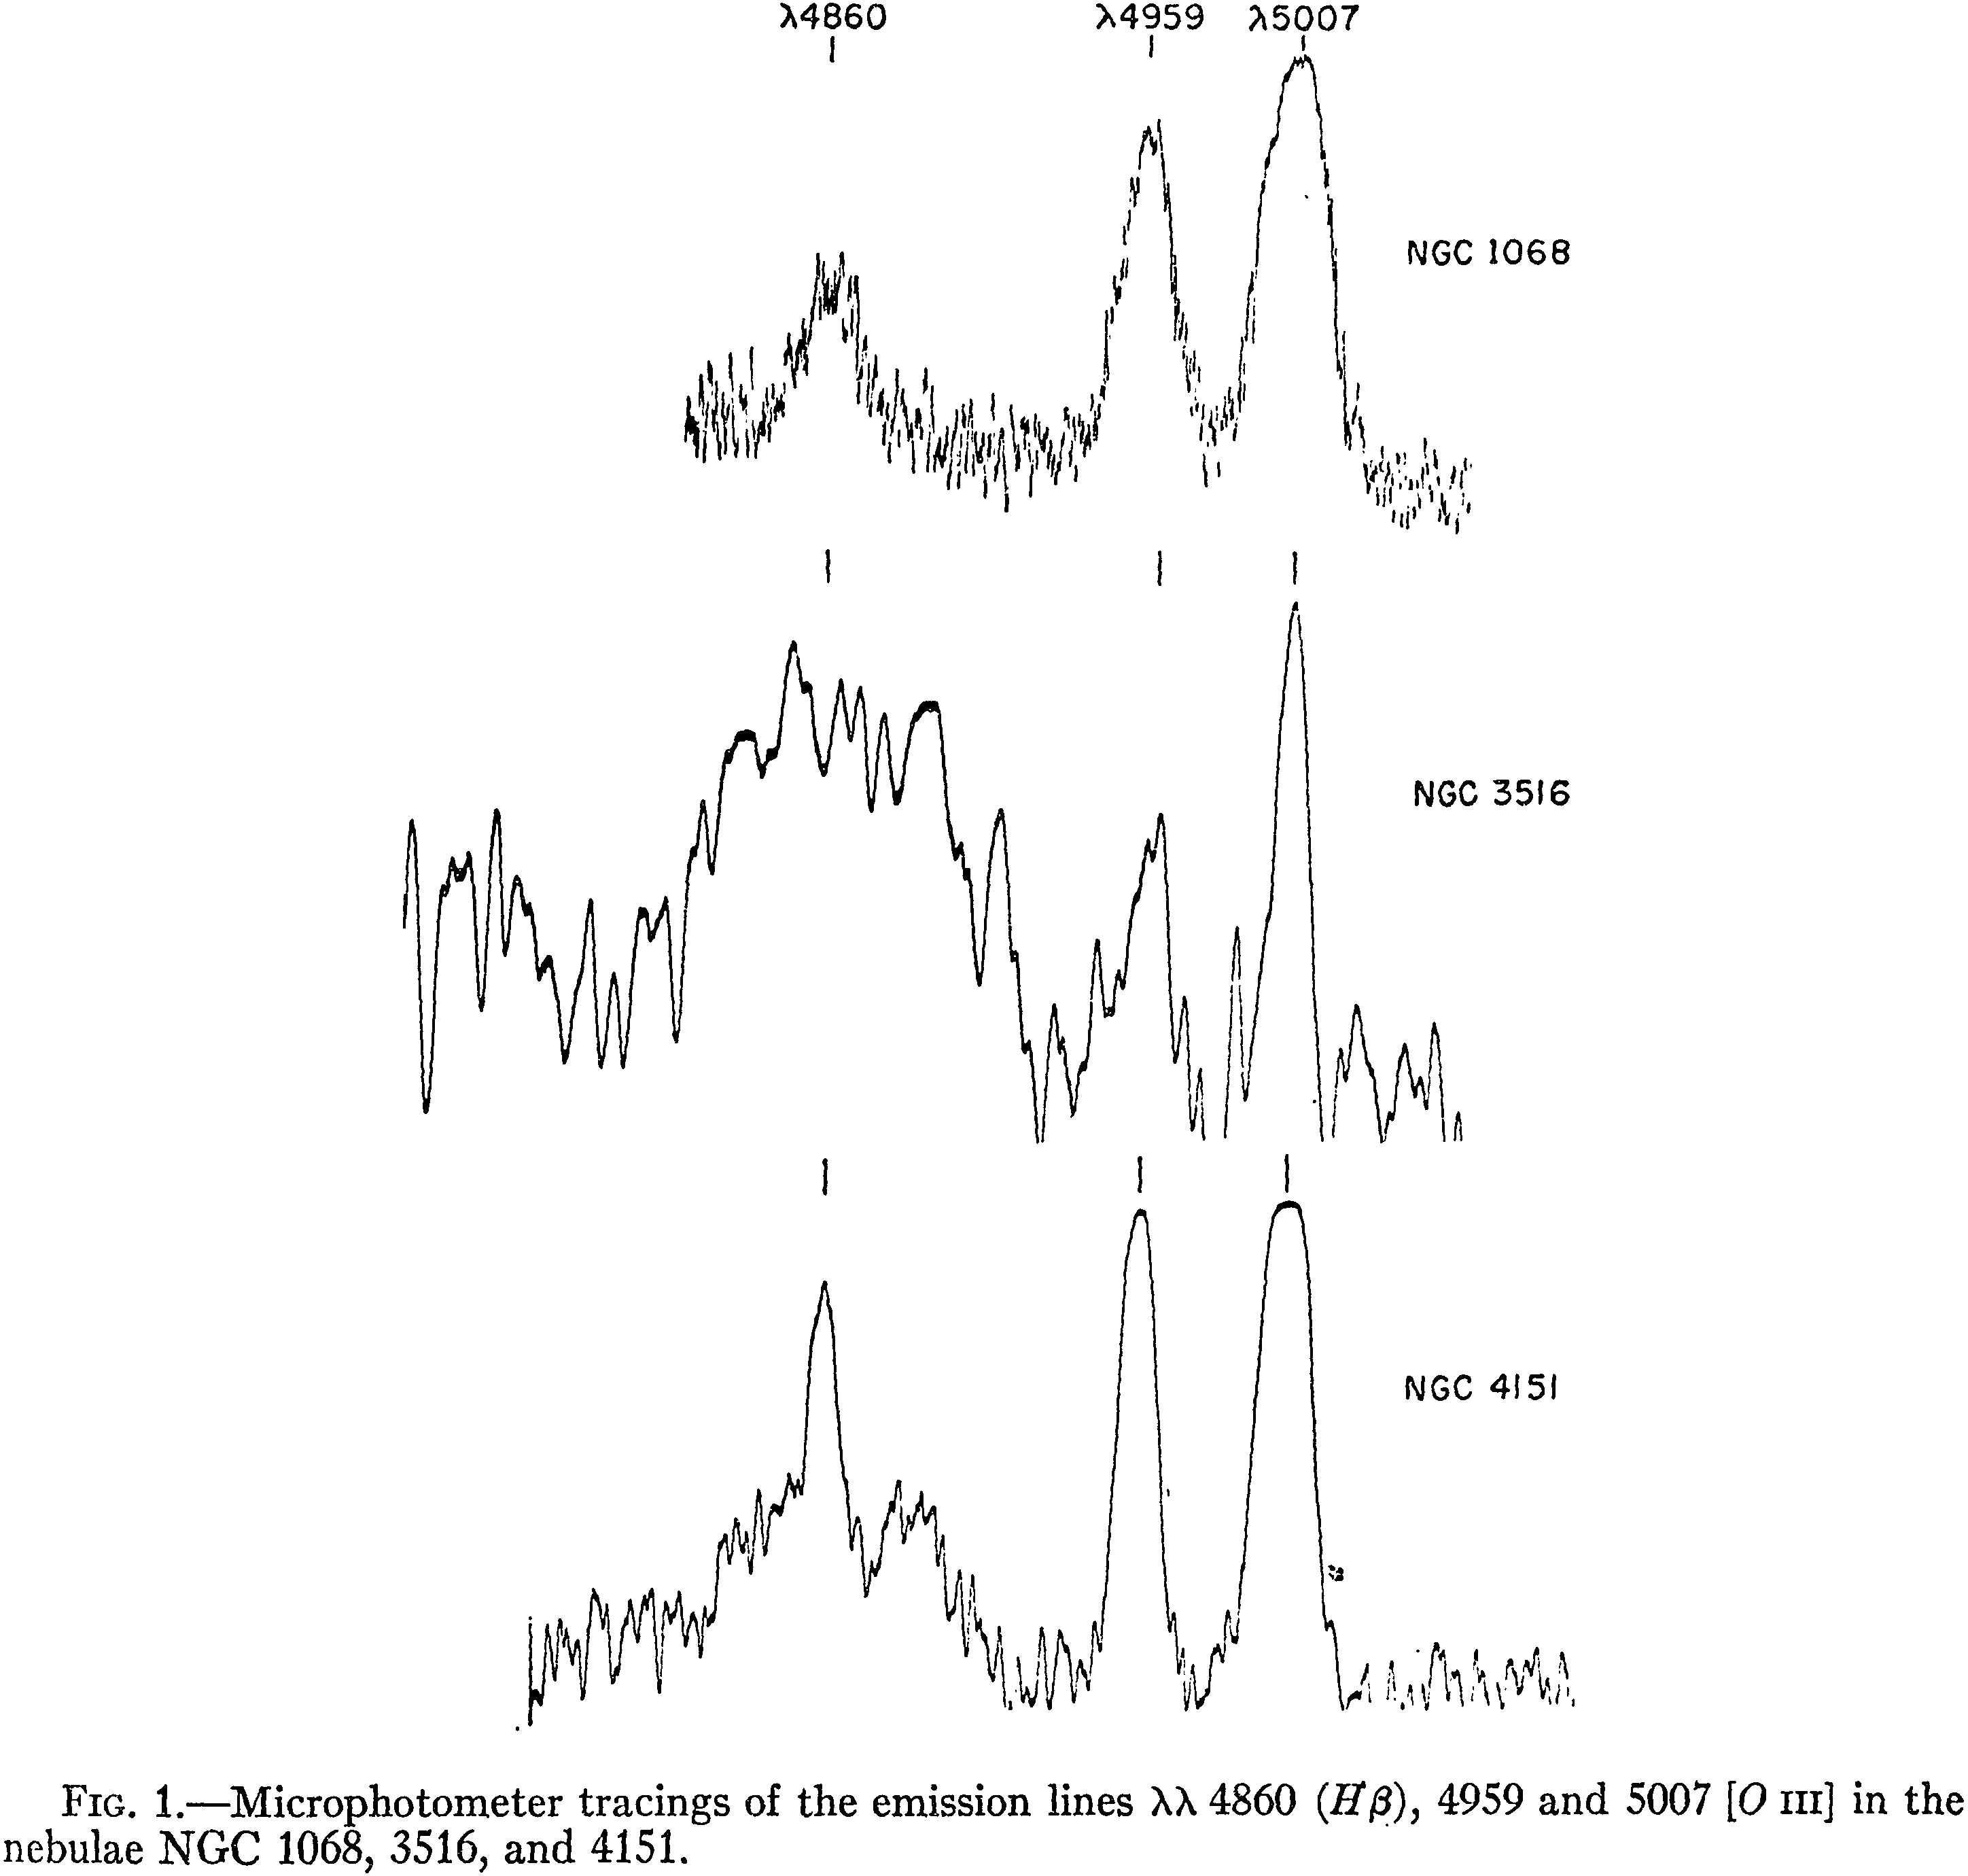
\includegraphics[width=0.5\textwidth]{1943CMWCI-671-7.jpg}
    %\label{fig:}
    \caption{
        The first spectrum of a Seyfert galaxy was taken in 1943. Contributions
        from the Mount Wilson Observatory / Carnegie Institution of Washington,
        vol. 671, pp.7-7.
    }
\end{figure}

In the catalog of 3C sources, it was first observed that there was a large
population of highly blue “stars” with unknown large lines
(\SI{8000}{\km\per\s}), like in 3C~48 (first detection: \citet{Matthews1960},
identification: \citet{1963ApJ-138-30M}). Moreover it was noticed that those
objects where redshifted. \citet{1964ApJ-140-1G}, measured redshifts of
$z=0.45$ and $0.16$ for 3C~48 and 3C~273. Thus those objects have to be at
cosmological distances but with very high luminosity.

\begin{figure}[!ht]
    \centering
    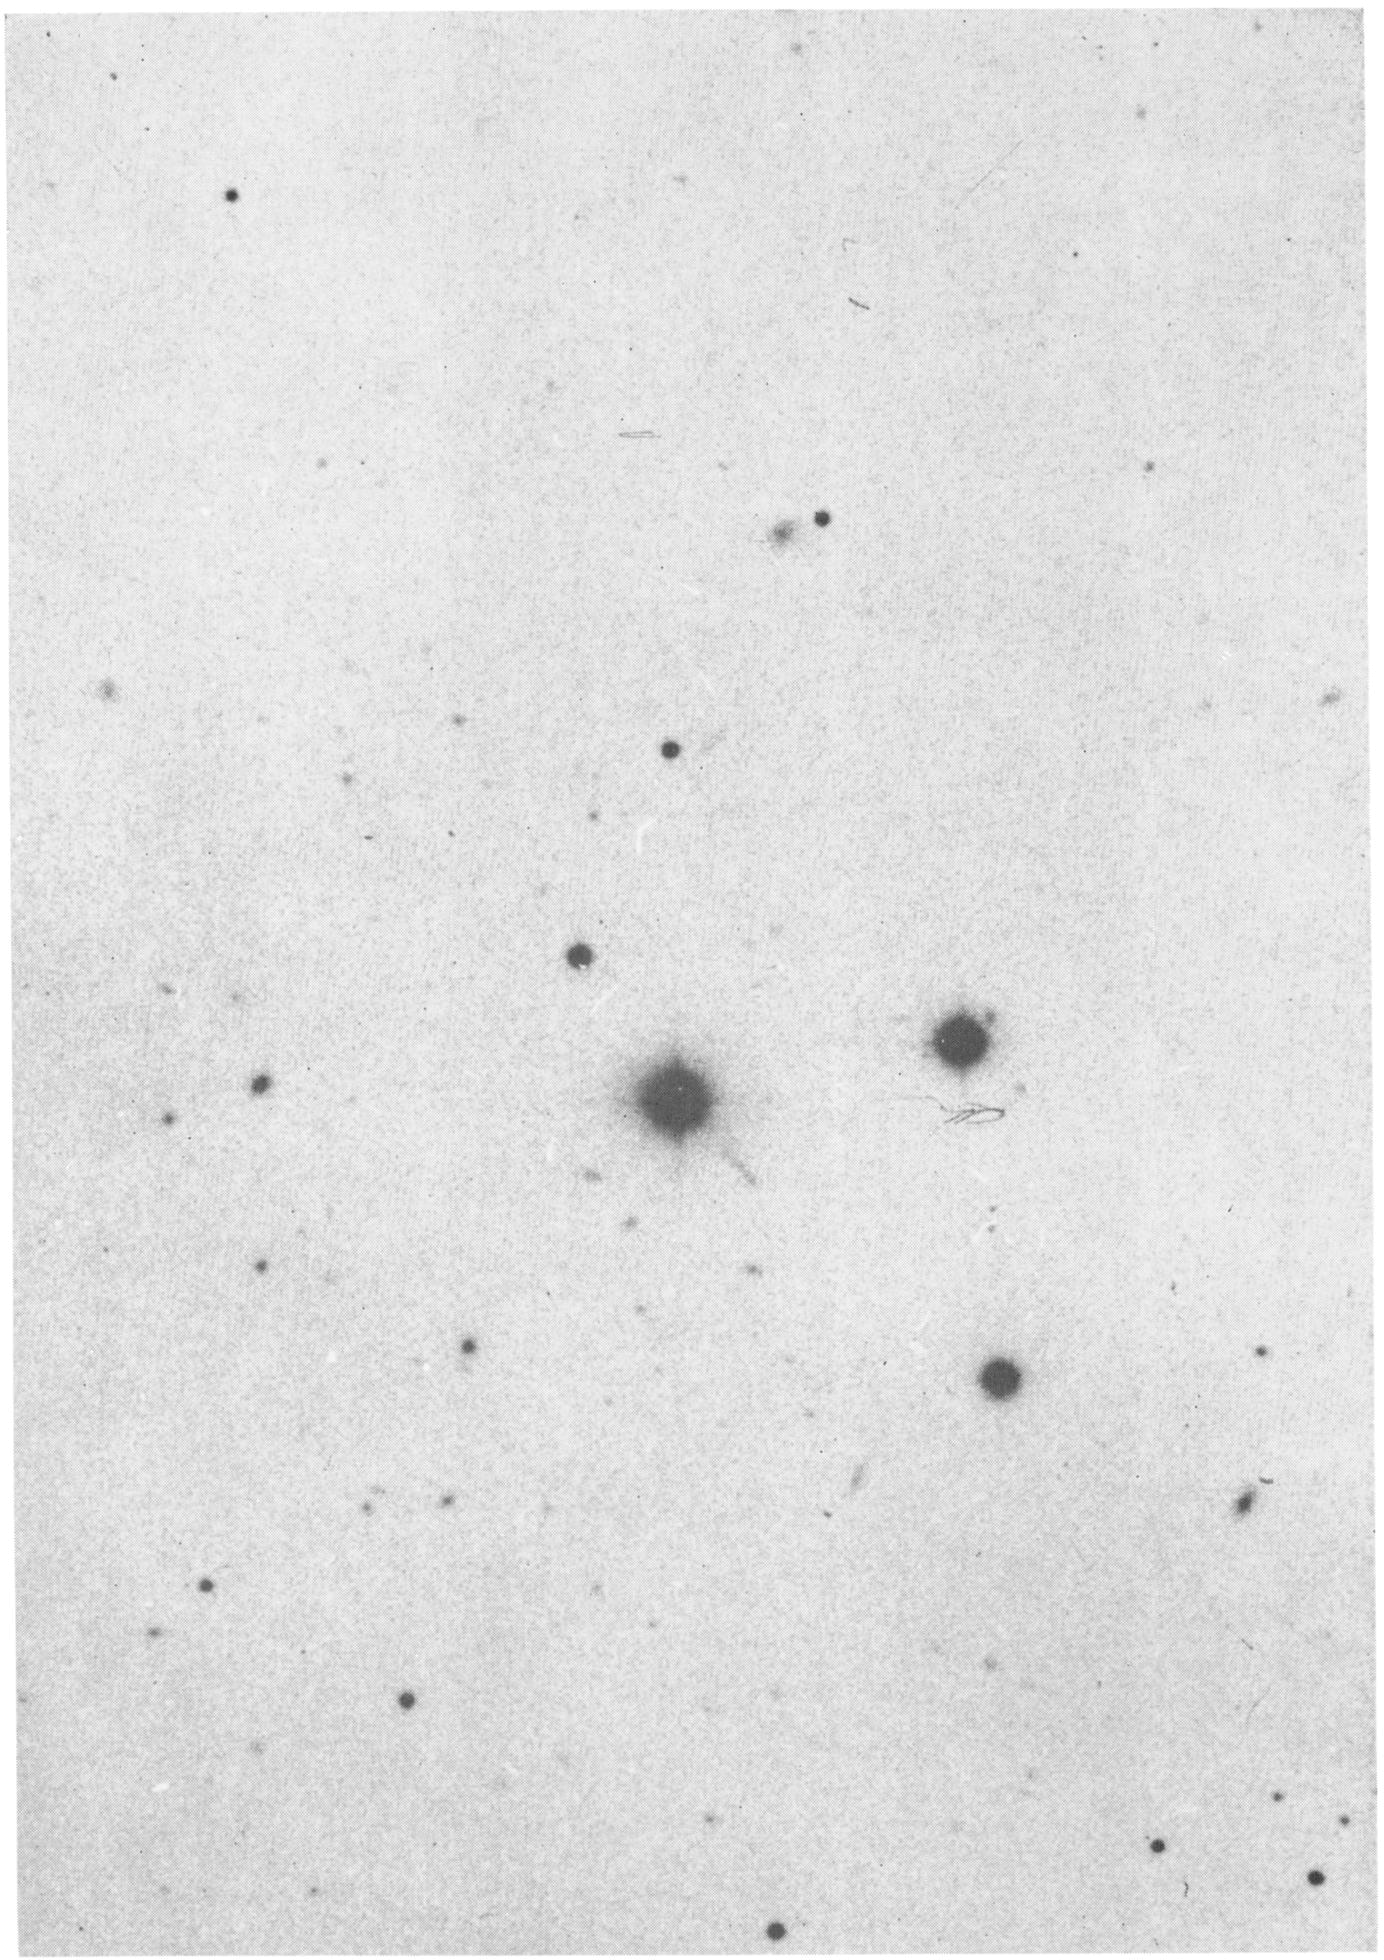
\includegraphics[width=0.5\textwidth,clip,trim=50mm 130mm 50mm 260mm]{1964ApJ-140-1G_1.jpg} % FIXME: You probably want to shrink or crop this one
    %\label{fig:}
    \caption{
        Enlarged portion of 200-inch photograph of 3C~273 (froam a 103a-D plate
        taken by A.~R.~Sandage); north is up, east to left. The weak narrow jet
        visible in position angle \SI{223}{\degree} reaches to about 20 inches
        from the quasi-stellar object. From \cite{1964ApJ-140-1G}.
    }
\end{figure}

\begin{figure}[!ht]
    \centering
    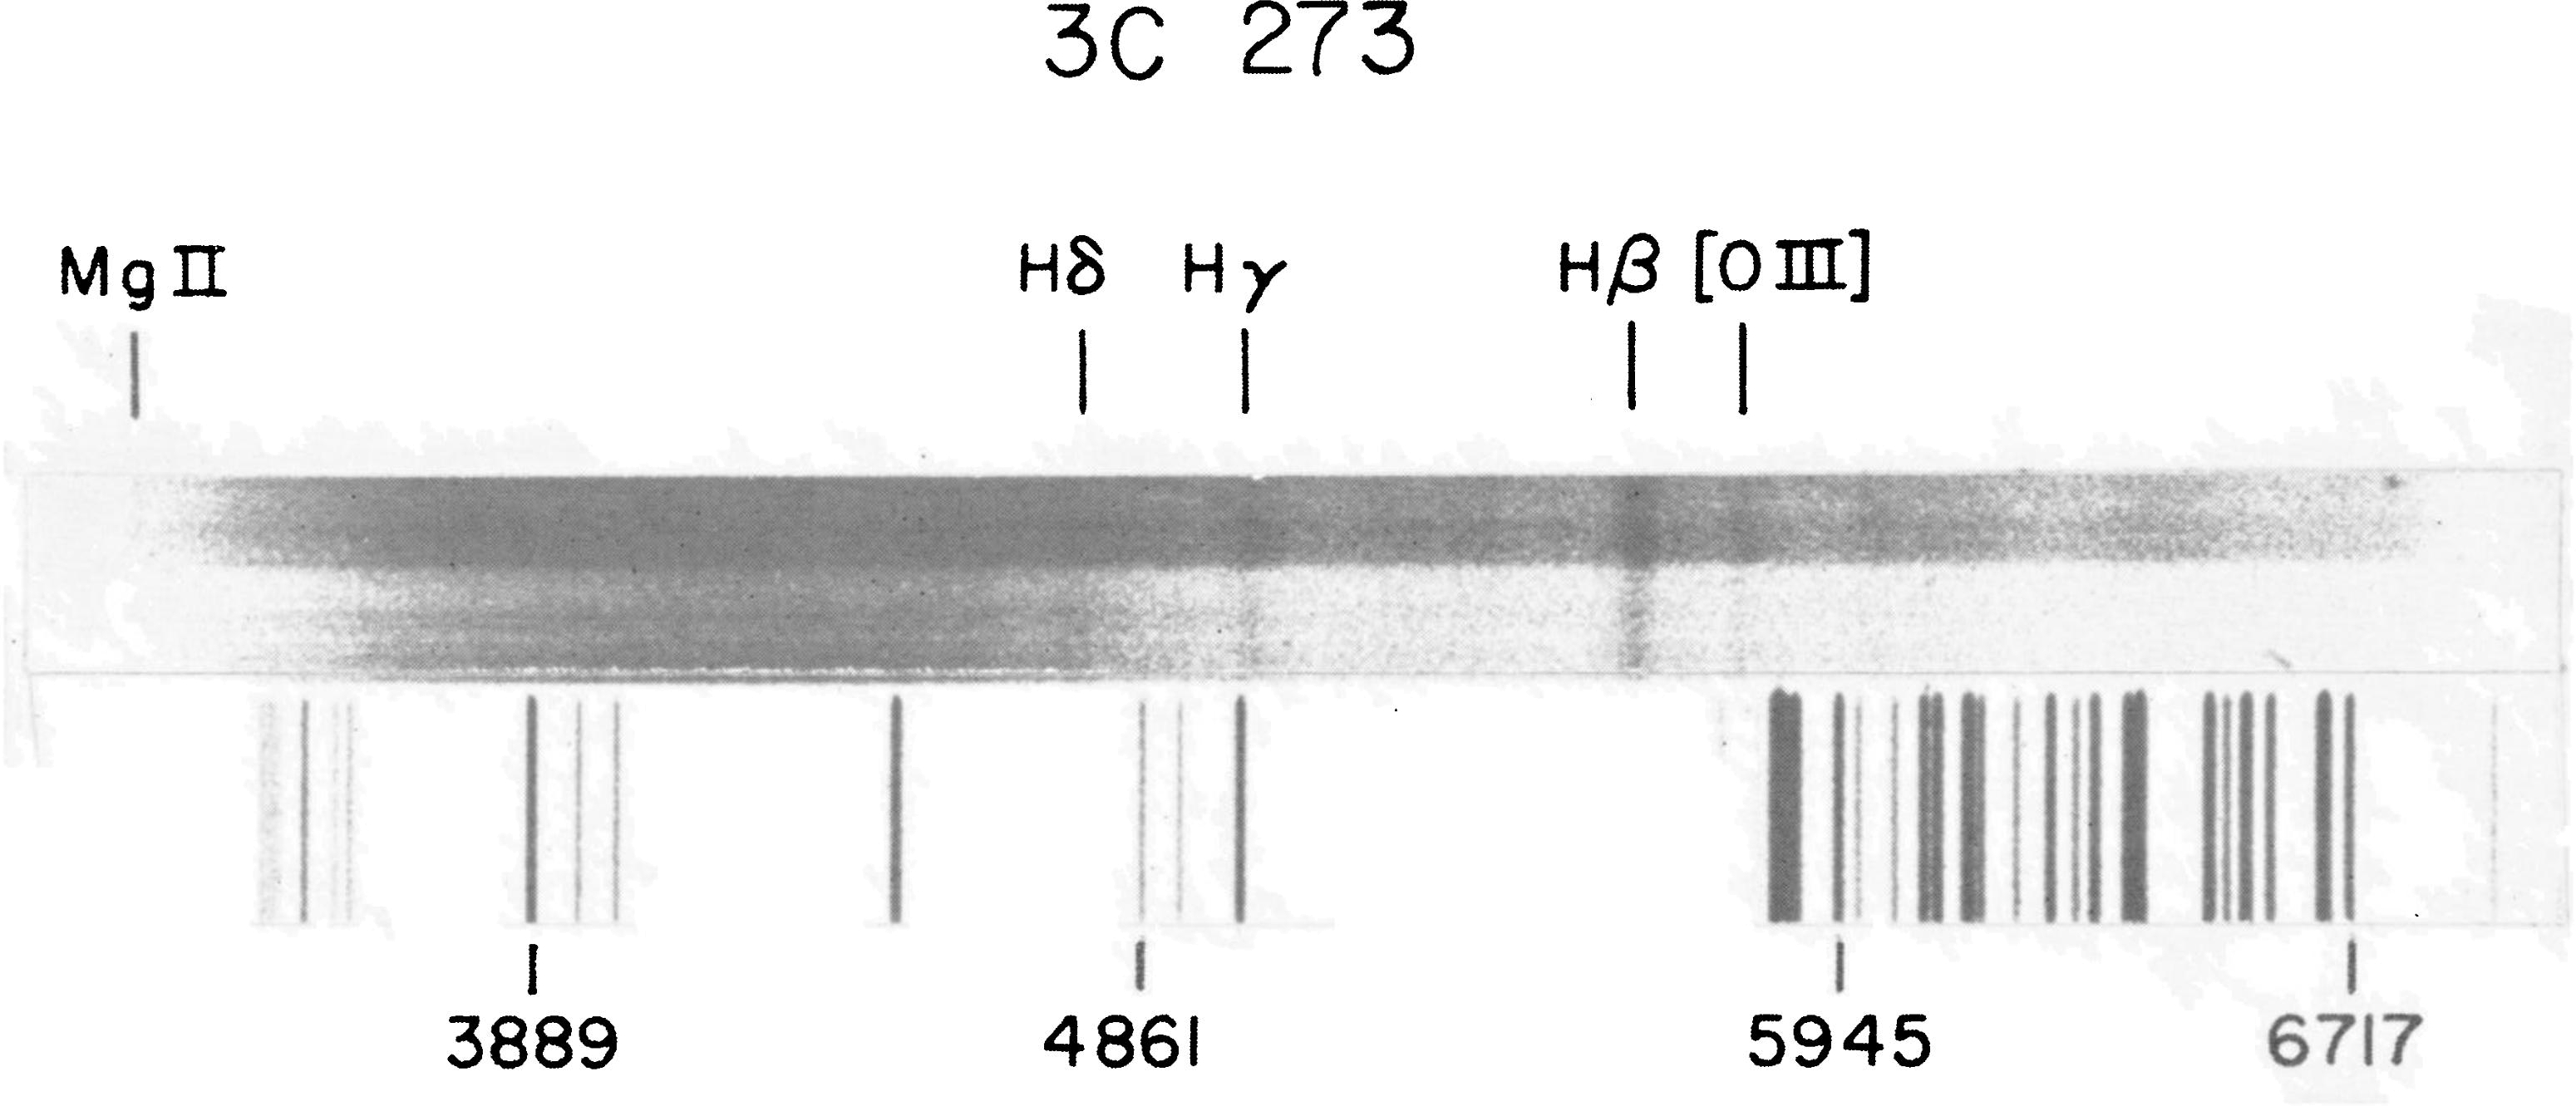
\includegraphics[width=0.9\textwidth]{1964ApJ-140-1G_2.jpg}
    %\label{fig:}
    \caption{
        Spectrum of the quasi-stellar object 3C 273B,
        \SI{400}{\angstrom\per\mm} original, 103a-F, January 23, 1963. The
        comparison spectrum is H + He + Ne. Exposure over the upper half of
        slit was three times that over the lower half. Redshifted emission
        lines of H and [O \textsc{III}] are indicated; also the barely visible
        line of Mg \textsc{II}, confirmed on denser exposures. From
        \cite{1964ApJ-140-1G}.
    }
\end{figure}

Seyfert galaxies are usually normal spiral galaxies. They have a radio core,
which fluctuates in brightness. Because of the intense radio core they are
classified in the larger family of Active Galactic Nuclei. A long debate
occurred initially to know if the radio emission could be constructed form star
burst emission. Nowadays, the radio core and the whole spectrum (because we
have multi-wavelength observations) is understood as the result of the emission
of an accretion disk with or without outflows around a central supermassive
black hole.

As radio-quiet objects represent $\sim \SI{90}{\percent}$ of the “average” AGN,
they also represent a very large source for the gamma ray background emission
at low level.

\begin{figure}[!ht]
    \noindent
    \begin{minipage}{.49\textwidth}
        %\includegraphics[width=\textwidth]{}
        \FIXME{Missing figure?} % There is a NGC4261 core pictures in the original document, but I can’t see any reason to include it here
        %\label{fig:}
        %\caption{}

        \vspace{1ex}
        \caption{
            NGC4258 Massive Black Hole \& Accretion Disk. Image courtesy of
            NRAO/AUI and L. Greenhill (Harvard-Smithsonian Center for
            Astrophysics).\vspace{1ex}\\
            NGC 4258 is a Seyfert galaxy in the constellation Ursa major. It is
            generally agreed to have at its heart a supermassive black hole
            some 39 million times more massive than the Sun. Gas orbiting this
            black hole has formed a warped disk nearly two light years in
            diameter. By measuring extremely small shifts in the positions of
            \ce{H_2O} masers (water vapor that amplifies microwave radio
            emissions) located in this disk, scientists have been able to
            measure the distance to this galaxy as 23.5 million light years, a
            measurement the scientists say is accurate to within a million
            light years.\vspace{1ex}\\
            The disk is viewed nearly edge-on from Earth and orbits the black
            hole at a speed of more than 2 million miles per hour. Using the
            Very Long Baseline Array, the astronomers observed the Doppler
            shift of the masers at the disk's sides at 4 to 8 month intervals
            over more than three years. This shift, or “proper motion”,
            combined with previous observations in which astronomers had
            measured the speed of the orbiting disk and ascertained the mass of
            the black hole, has enabled the scientists to make the distance
            determination.\vspace{1ex}\\
            Previous observations using Cepheid variable stars and the Hubble
            Space Telescope had set the distance at 27 or 29 million light
            years. The difference in these two distance determinations will
            make a significant impact on future calculations of the size and
            age of the Universe.
        }
    \end{minipage}%
    \hfill
    \begin{minipage}{.49\textwidth}
        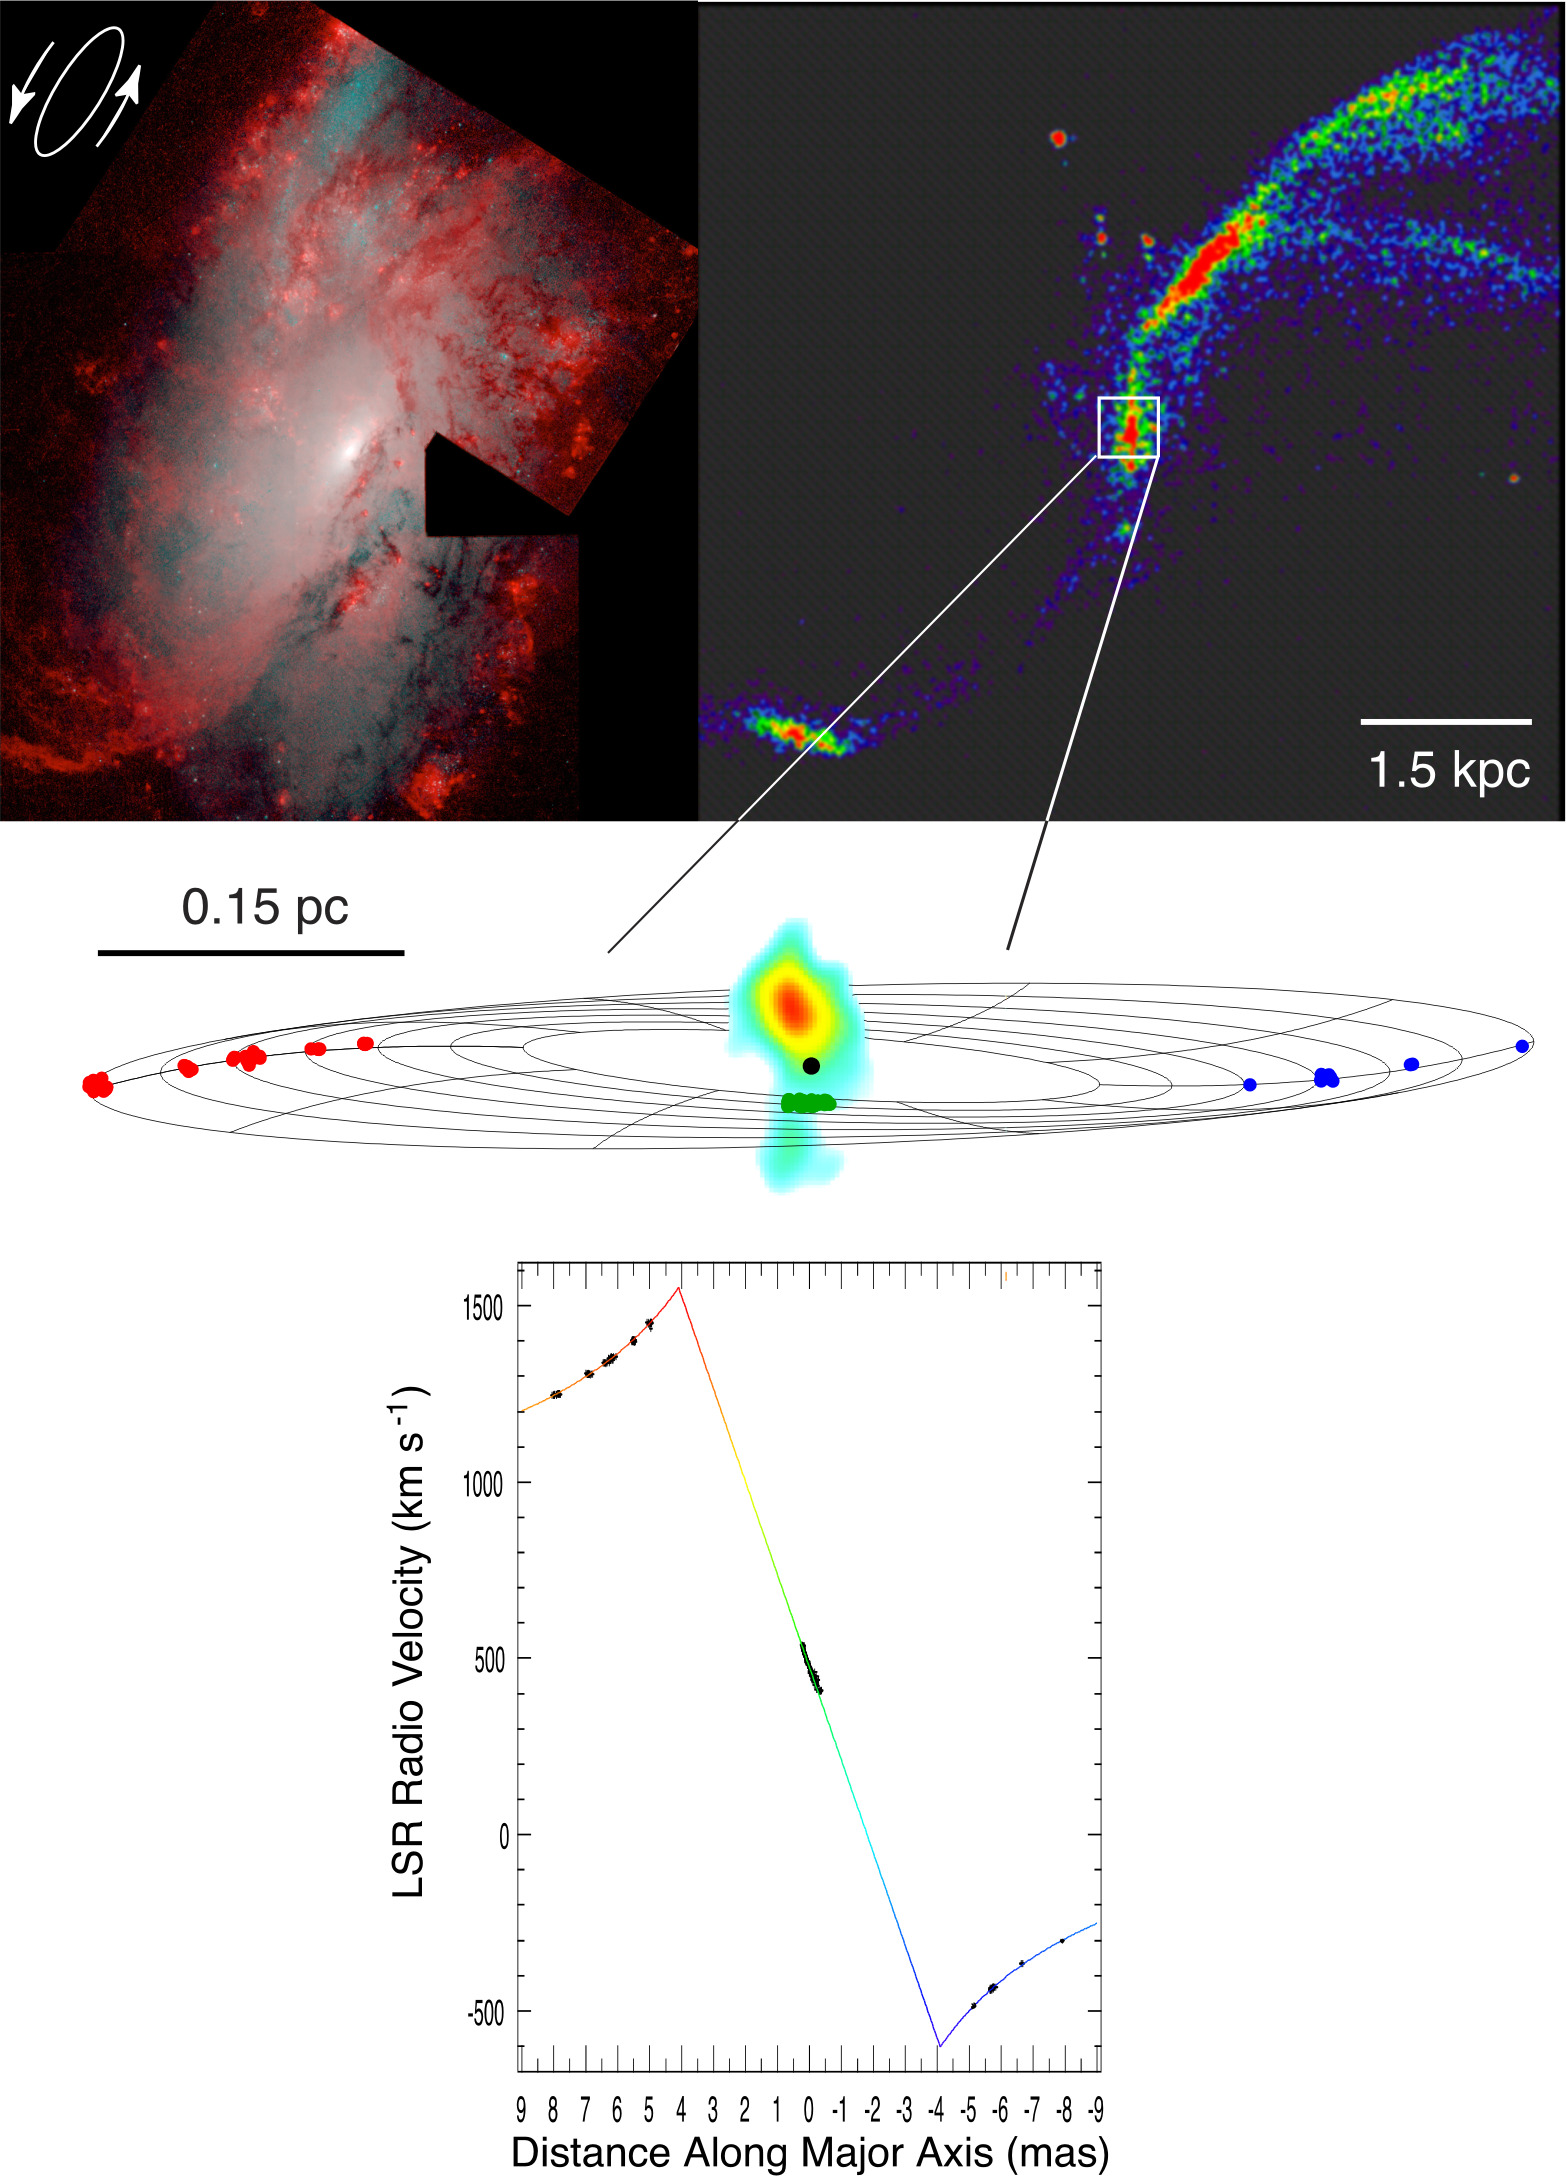
\includegraphics[width=\textwidth]{ngc4258_combo_hst_hi.jpg}
        %\label{fig:}
    \end{minipage}
\end{figure}

\subsubsection{Radio Loud, Narrow Line Radio Galaxies}

Conversely to Seyfert galaxies, radio loud galaxies have an extended radio
emission in addition to the radio core. They are usually seen in giant
elliptical galaxies and not spiral ones. From our observational point of view,
the most powerful sources as such are of course quasars and BL Lac objects.
However the most striking structure is seen in radio galaxies of Fanaroff Riley
types.

\begin{figure}[!ht]
    \noindent
    \begin{minipage}{.6\textwidth}
        \centering
        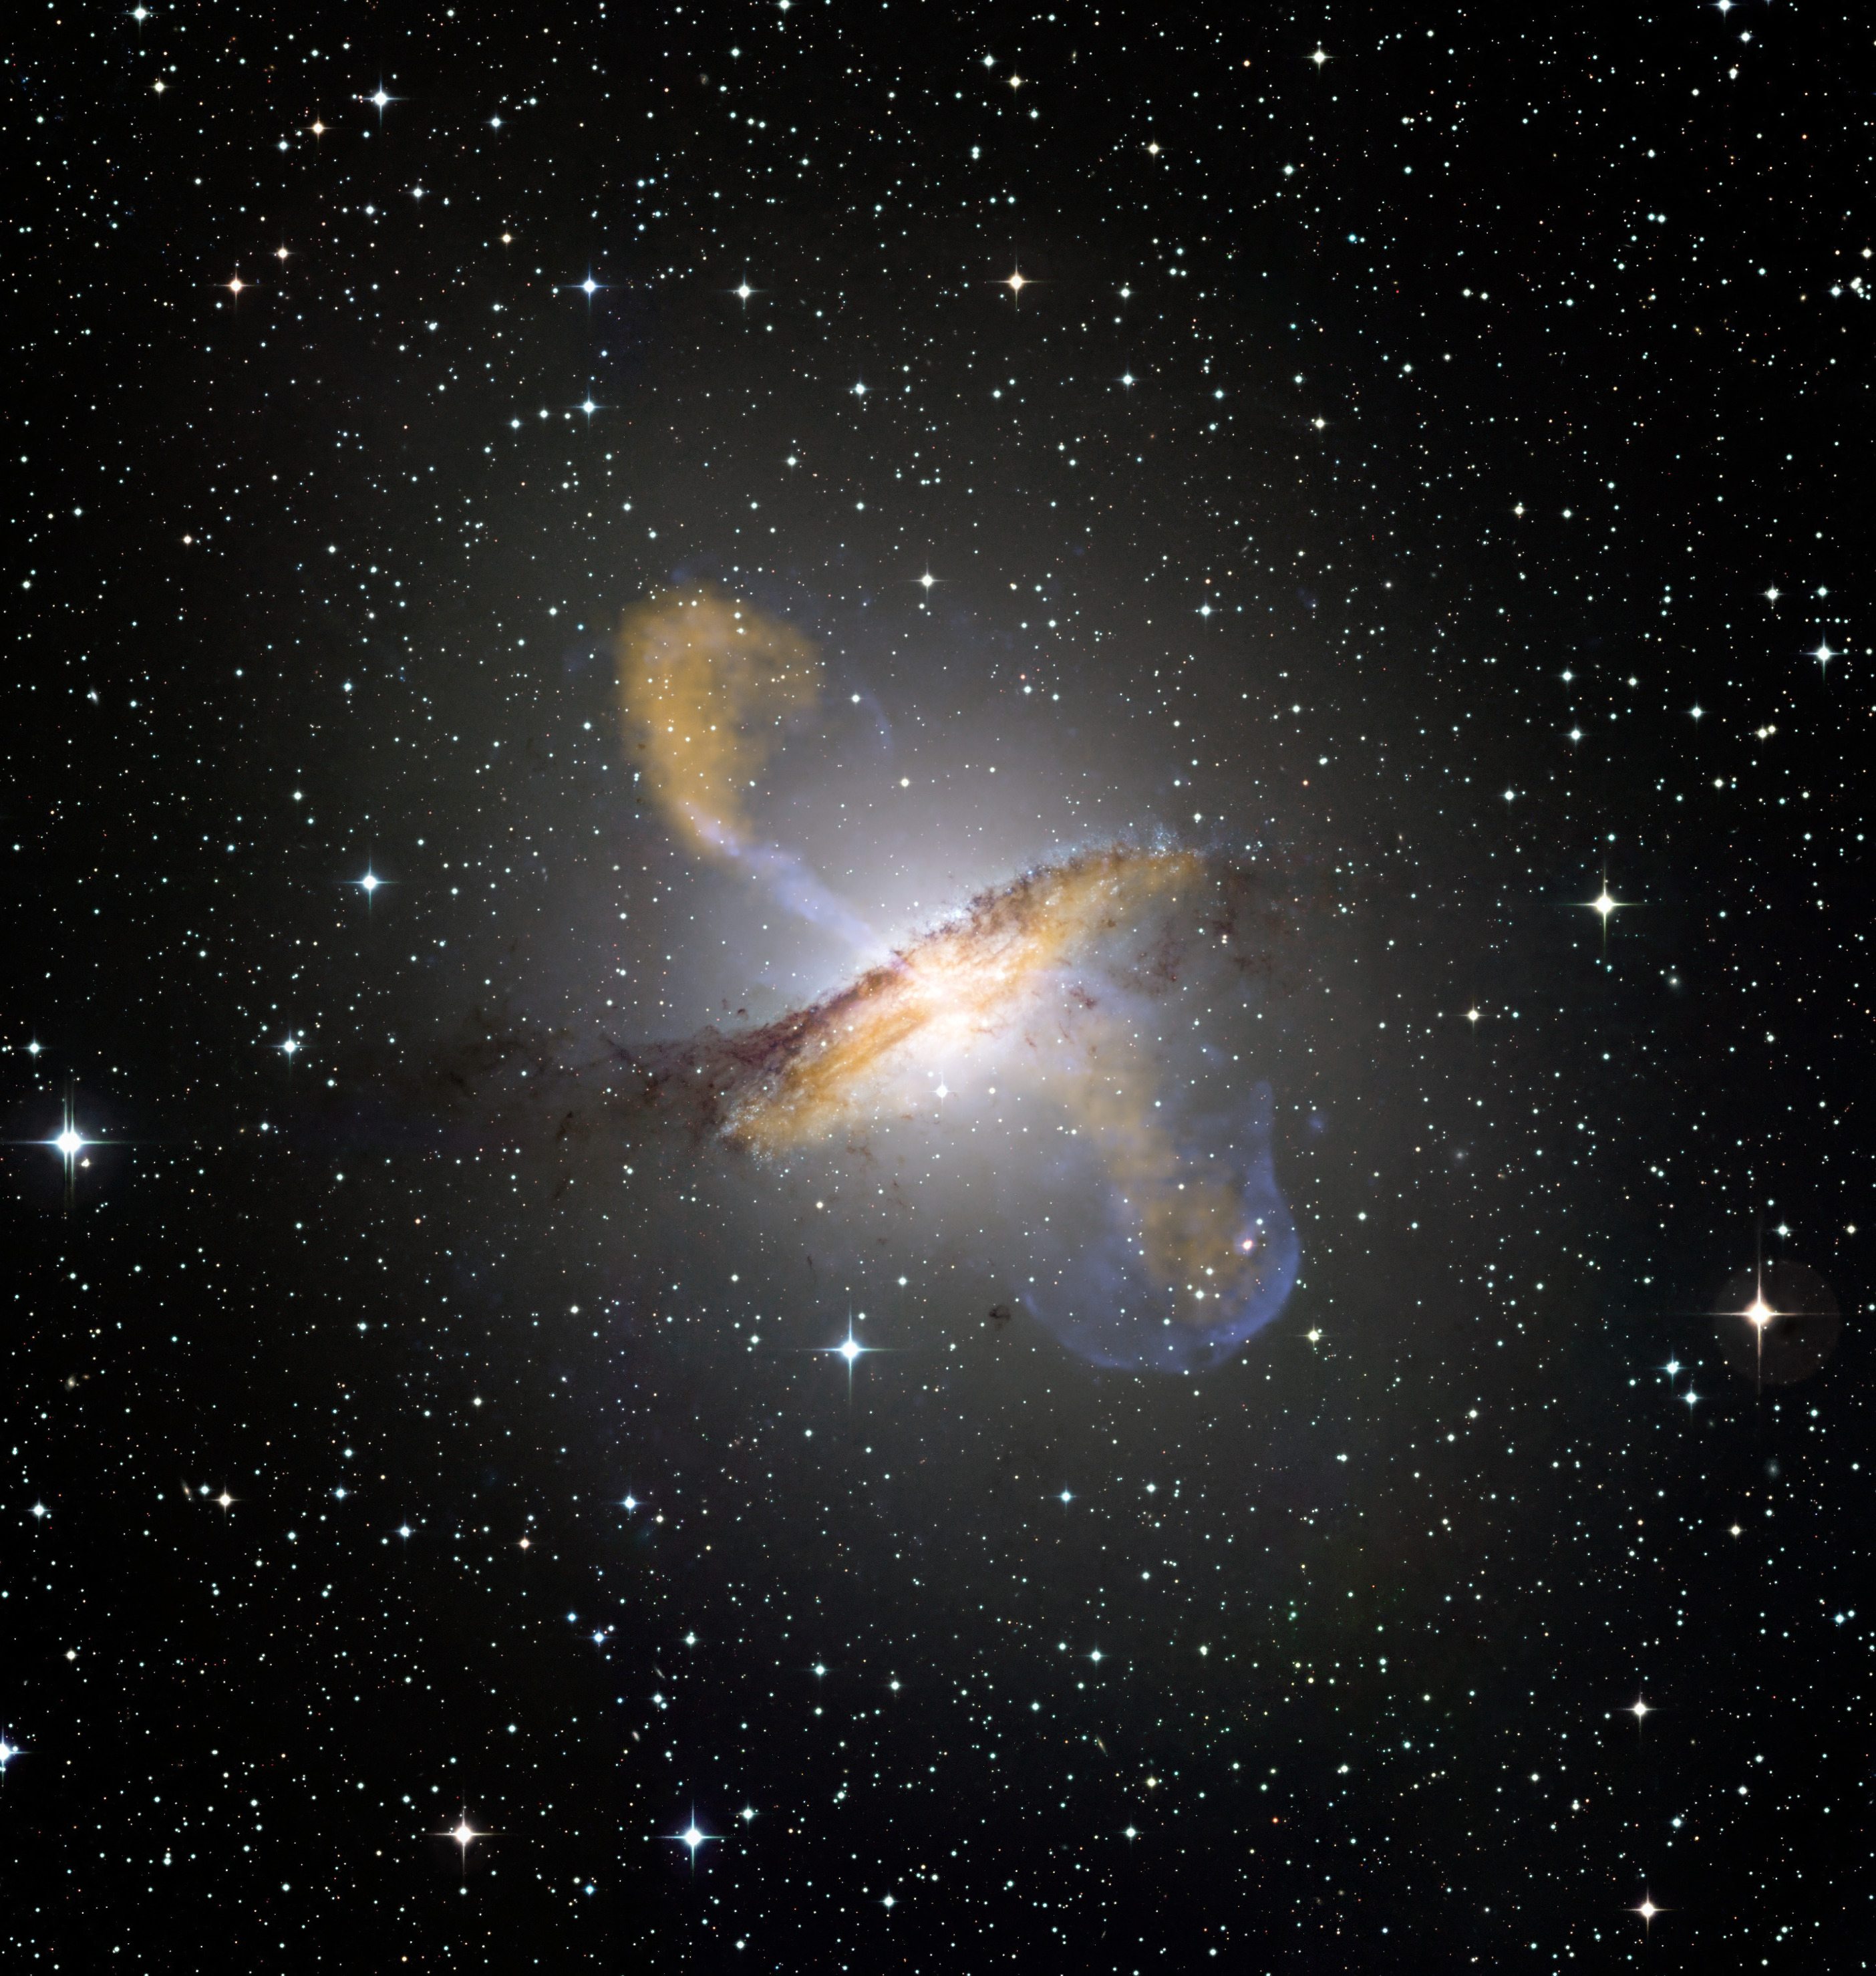
\includegraphics[width=0.8\textwidth]{eso0903a.jpg}
        %\label{fig:}
    \end{minipage}%
    \hfill
    \begin{minipage}{.4\textwidth}
        \caption{
            Centaurus A*. ESO/WFI (Optical); MPIfR/ESO/APEX/A.Weiss et al.
            (Submillimetre); NASA/CXC/CfA/R.Kraft et al. (X-ray).\vspace{1ex}\\
            Colour composite image of Centaurus A, revealing the lobes and jets
            emanating from the active galaxy’s central black hole. This is a
            composite of images obtained with three instruments, operating at
            very different wavelengths. The 870-micron submillimetre data, from
            LABOCA on APEX, are shown in orange. X-ray data from the Chandra
            X-ray Observatory are shown in blue. Visible light data from the
            Wide Field Imager (WFI) on the MPG/ESO \SI{2.2}{\m} telescope
            located at La Silla, Chile, show the stars and the galaxy’s
            characteristic dust lane in close to “true colour”.
        }
    \end{minipage}
\end{figure}

Radio loud sources and quasars have relativistic jets in addition to the
accretion disk, with bulk Lorentz factor $\Gamma=\nicefrac{1}{\sqrt{1-V^2/c^2}}$
of 3 to 10 or possibly higher.

\begin{figure}[!ht]
    \noindent
    \begin{subfigure}[t]{.495\textwidth}
        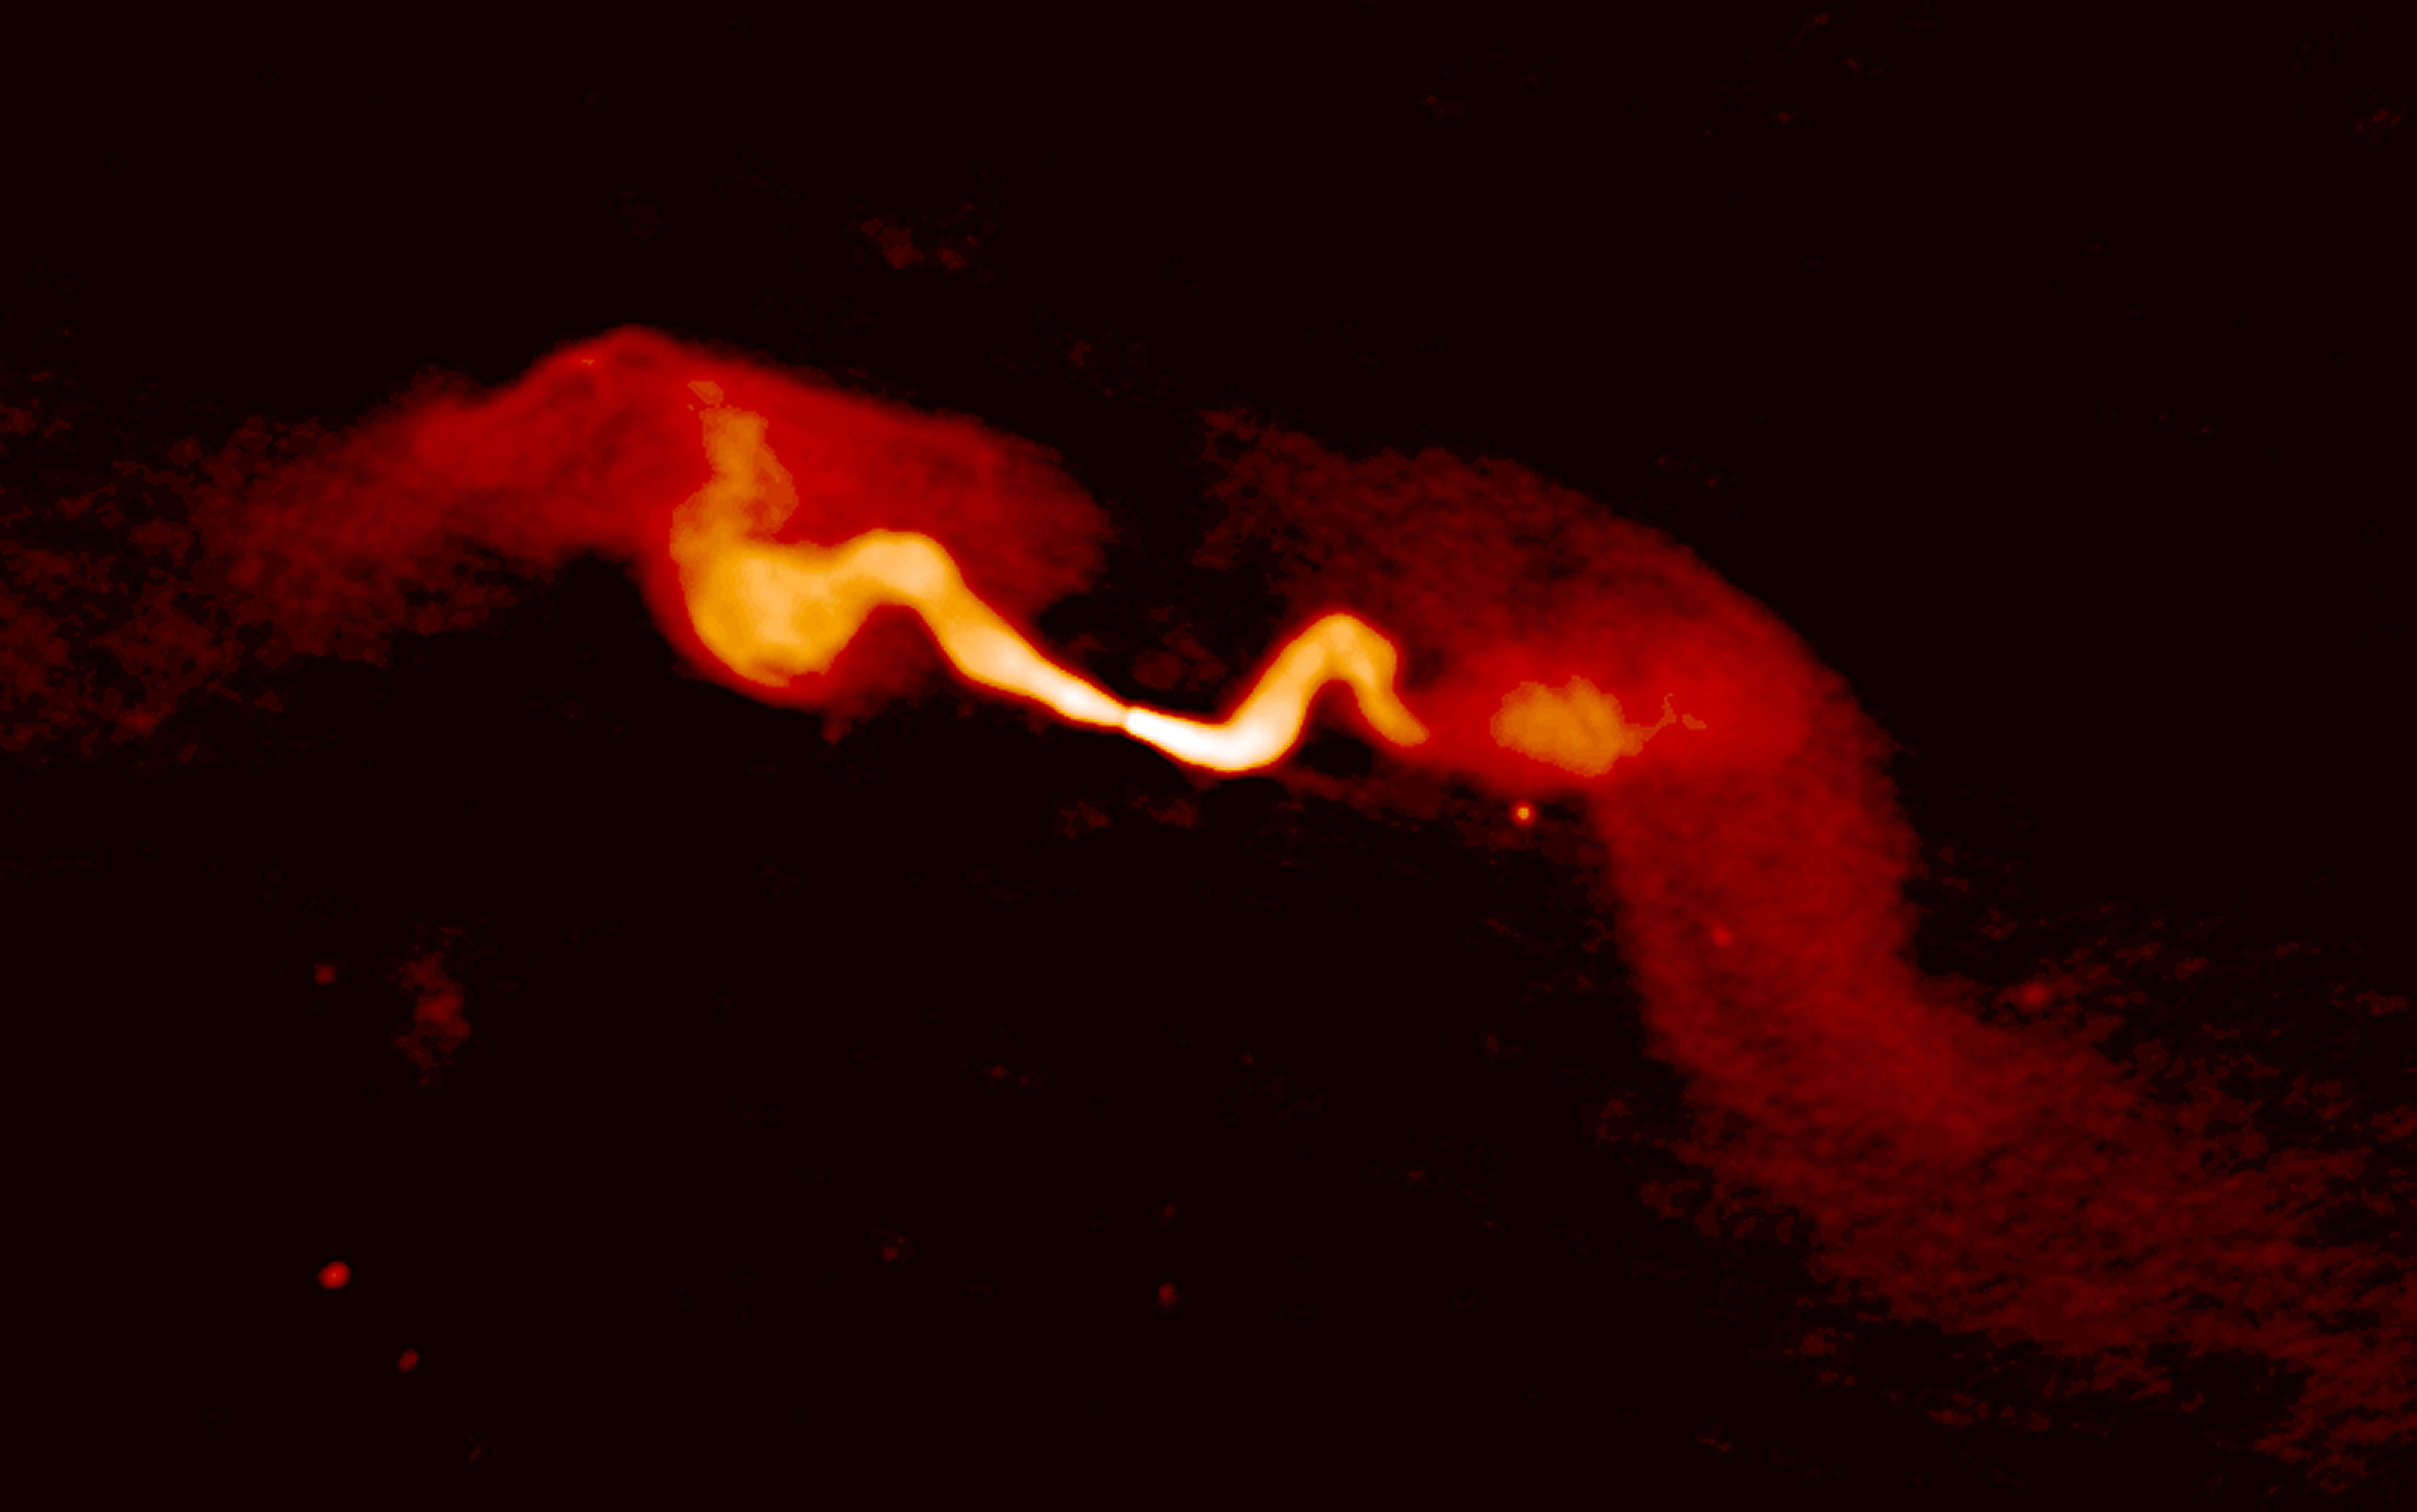
\includegraphics[width=\textwidth]{3c31lbcd_6in_hi.jpg}
        %\label{fig:}
        \caption{
            3C~31 radio galaxy, VLA (\SI{20}{\cm}), 1999.
            Image courtesy of NRAO/AUI.\vspace{1ex}\\
            This image shows the radio morphology of the radio galaxy 3C~31 (NGC
            383), the dominant galaxy of a prominent chain of galaxies. This
            system is a powerful radio source, with conical inner jets
            developing into distorted plumes, which stretch to a distance of
            300 kpc from the center of the galaxy (980,000 light years, for a
            Hubble constant of 100 km/s/Mpc). The radio emission is due to
            relativistic streams of high energy particles generated by the
            radio source at the center of the radio galaxy. Astronomers believe
            that the jets are fueled by material accreting onto a super-massive
            black hole. The high energy particles are shot into extra-galactic
            space at speeds approaching the speed of light, where they
            eventually balloon into massive radio plumes.
        }
    \end{subfigure}%
    \hfill
    \begin{subfigure}[t]{.495\textwidth}
        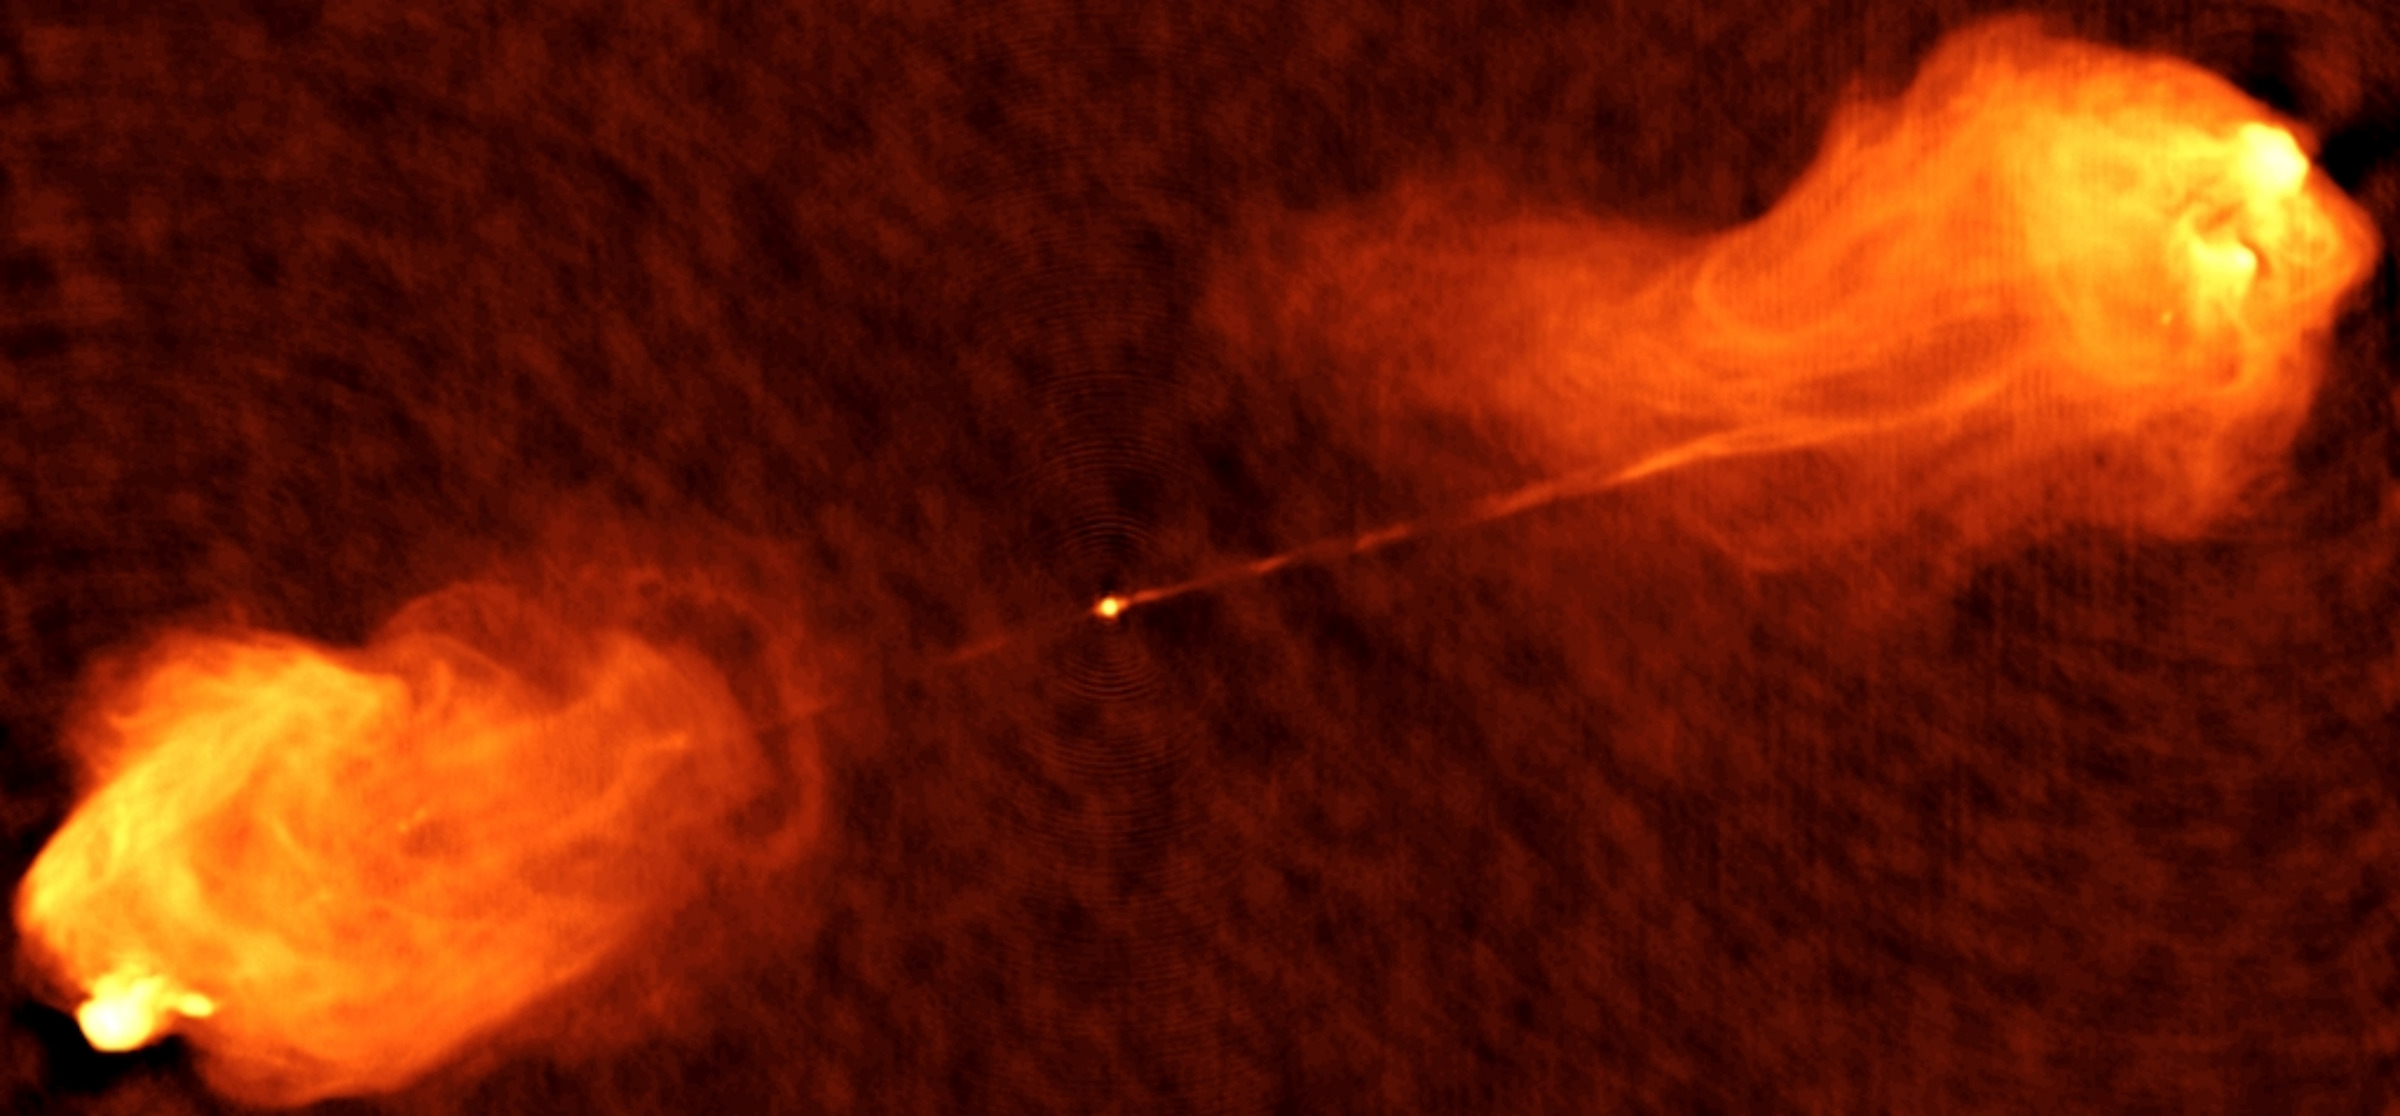
\includegraphics[width=\textwidth]{CygA-YellowOrange_hi.jpg}
        %\label{fig:}
        \caption{
            Cygnus A, VLA (\SI{6}{\cm}), 1983. Image courtesy of
            NRAO/AUI.\vspace{1ex}\\
            The radio source Cygnus A is produced in a galaxy some 600 million
            light-years away. The radio waves are coming from electrons
            propelled at nearly the speed of light through a long, thin “jet”
            at the core of the galaxy and deposited in giant “radio lobes”. It
            is here where the speeding electrons are trapped by the magnetic
            field around the galaxy to produce radio waves much like the Van
            Allen radiation belts around the Earth. Where did all the electrons
            come from? From the bright, small radio component in the center of
            the galaxy -- the location of a black hole.
        }
    \end{subfigure}
    \caption{
        FRI and FRII galaxies with morphological differences. 3C~31 is a
        typical FRI (left) and Cyg~A a typical FRII (right). The hot spots and
        the radio lobes are clearly seen. The one sided jet of Cyg A is visible
        as well as the two symmetric hot spots. The two jets of 3C~31 show that
        despites the two sided structure, the counter jet is less visible due to
        relativistic effects.
    }
\end{figure}

They are two types of radio loud galaxies, FRI and FRII.
\begin{itemize}
    \item FRI radio galaxies show elongated jets on both sides, on the
          \si{\kpc} scale terminated with two radio lobes (spatially extended
          structure). On the \si{\pc} scale, we see one-sided jets with
          relativistic speeds. On the \si{\kpc}, the jet is sub-relativistic
          and has decelerated.
    \item FRII radio galaxies are one sided and relativistic on the \si{\pc}
          and the \si{\kpc} scales. The are more powerful and terminated with
          two hot spots. This implies that, although the visible jet is one
          sided, counter jet exist but is invisible because it is not
          relativistically beamed.
    \item HYMORS is a new class of FR galaxies, which are FRI on one side and
          FRII on the other side. This may be explained if the environment
          plays an important role.
\end{itemize}

\begin{figure}[!ht]
    \centering
    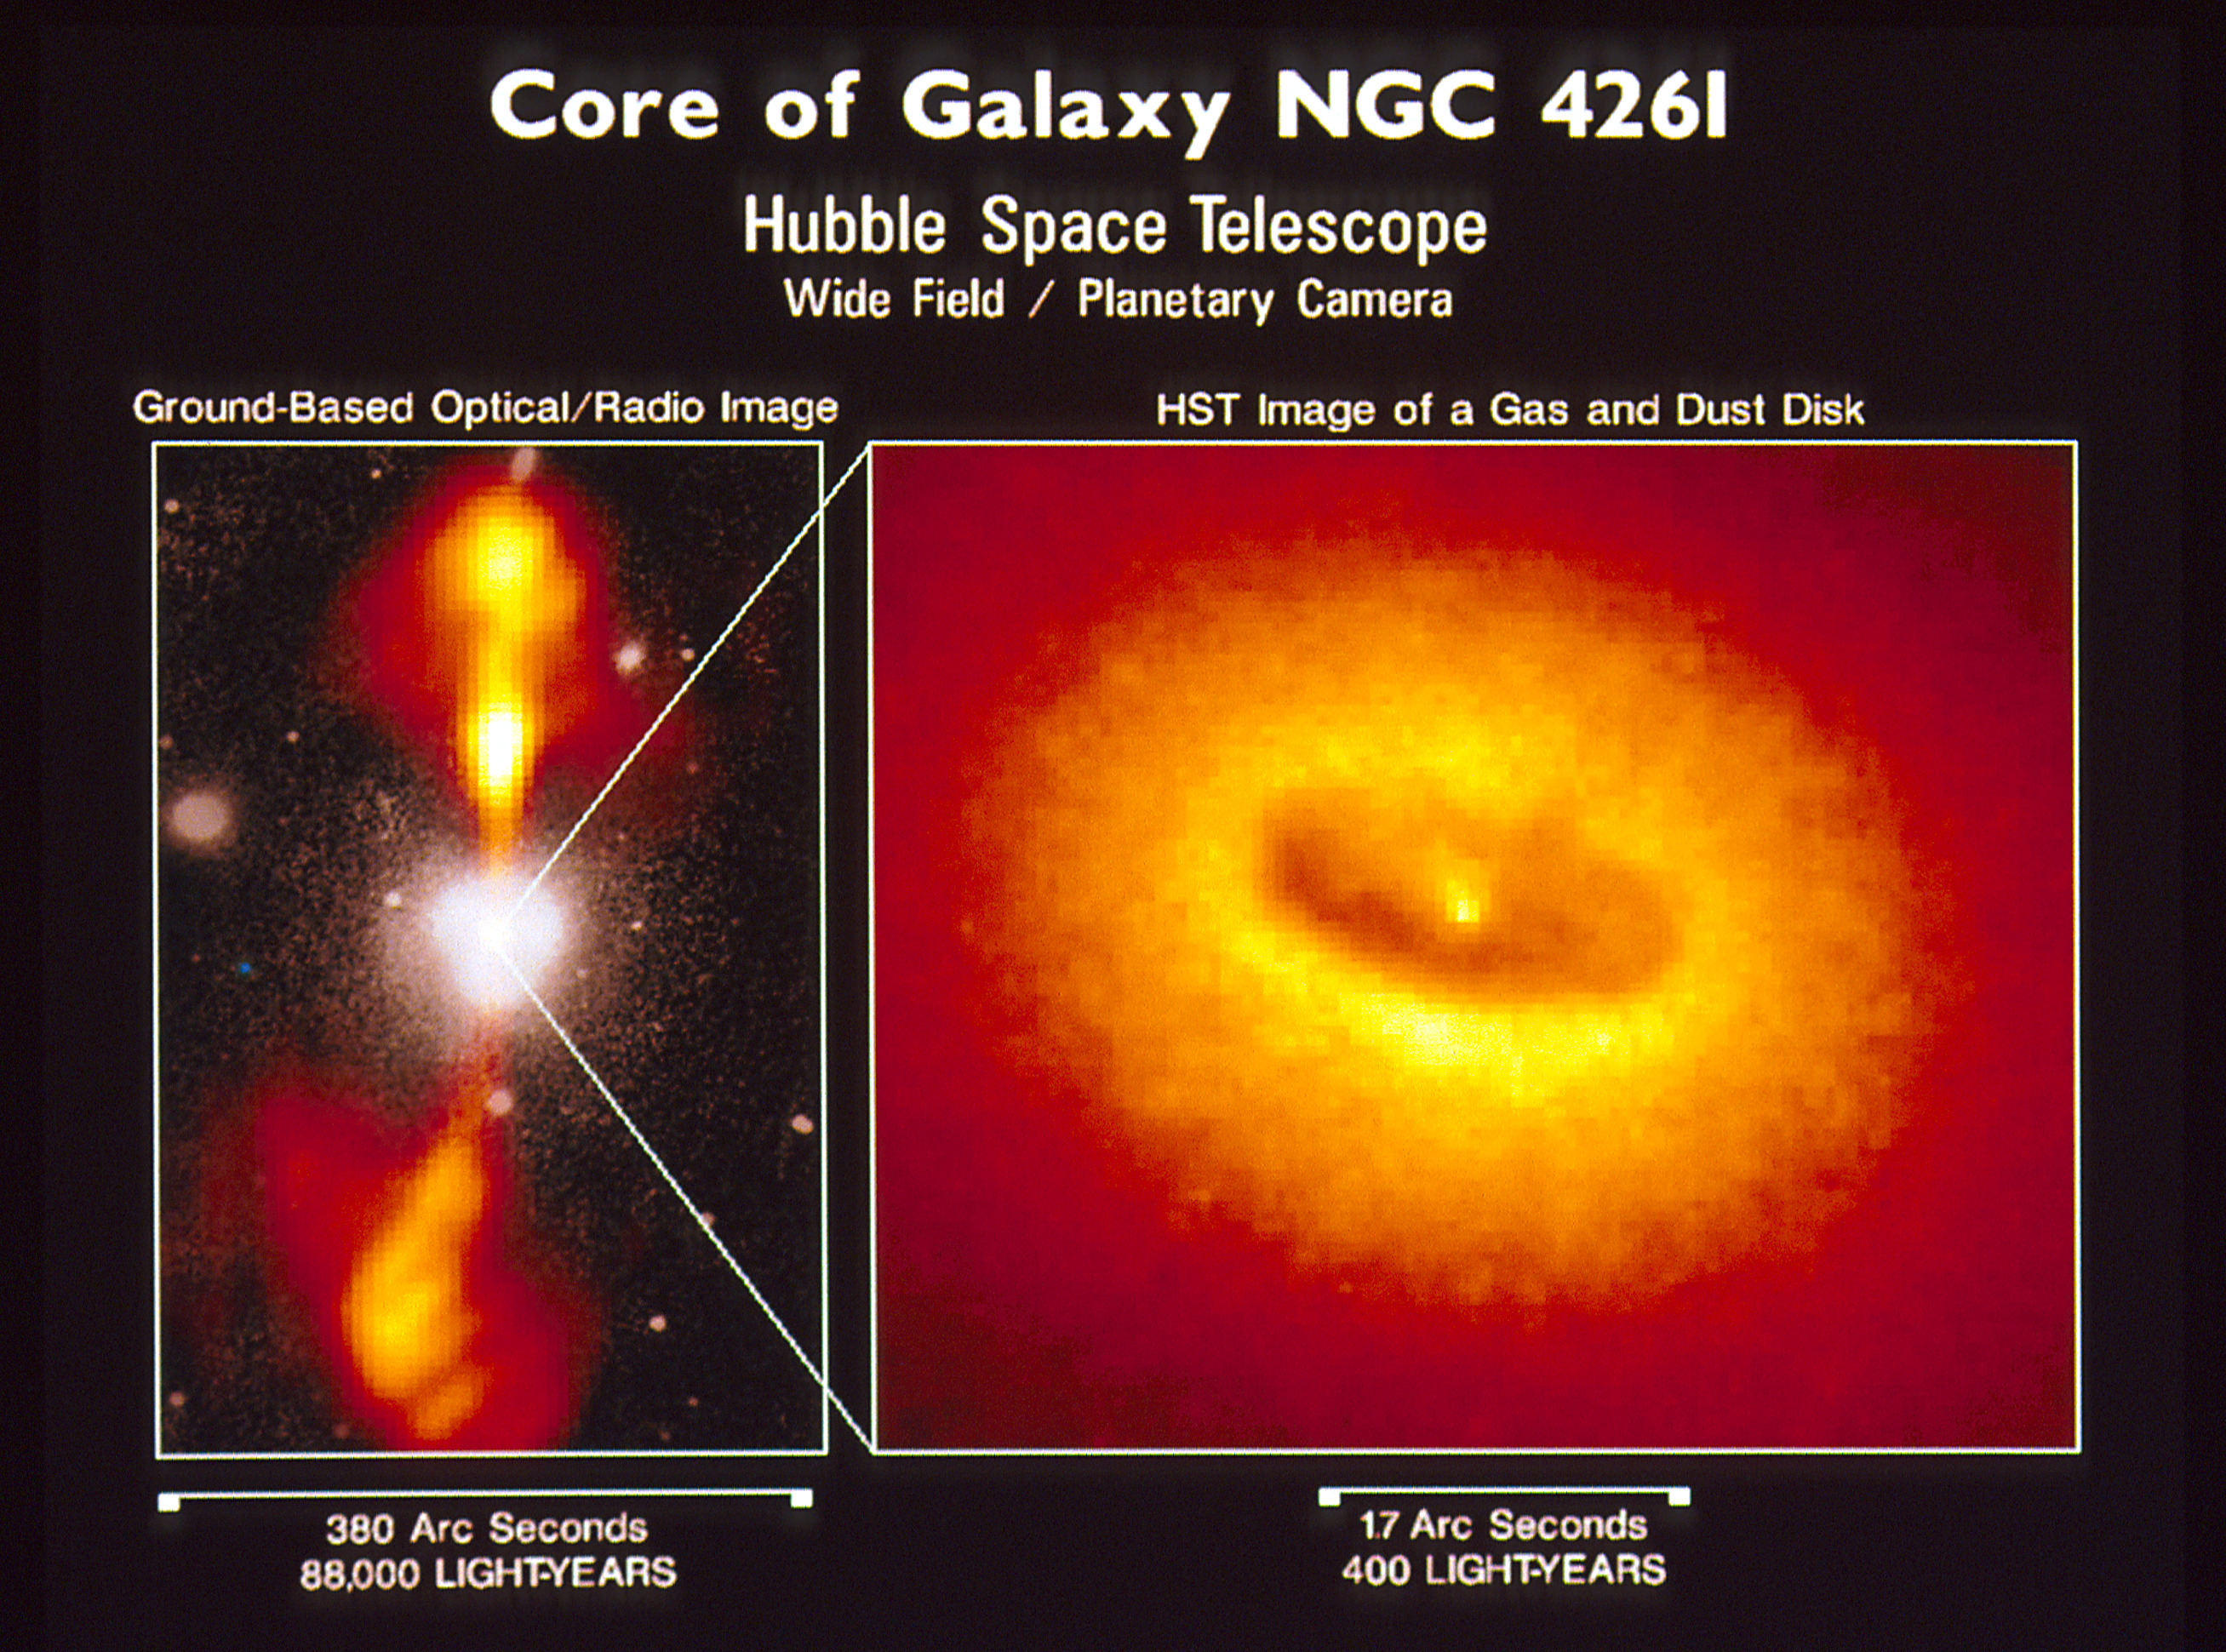
\includegraphics[width=0.6\textwidth]{hs-1992-27-b-full.jpg}
    %\label{fig:}
    \caption{
        NGC 4261 is another FRI.
        National Radio Astronomy Observatory, California Institute of
        Technology (left). Walter Jaffe/Leiden Observatory, Holland
        Ford/JHU/STScI, and NASA (right).%\vspace{1ex}\\
%        (Left) Ground-based Composite Optical/radio View of Elliptical Galaxy
%        NGC 4261.\vspace{1ex}\\
%        The giant elliptical galaxy NGC 4261 is one of the 12
%        brightest galaxies in the Virgo Cluster, located 45 million light-years
%        away. Photographed in visible light [white] the galaxy appears as a
%        fuzzy disk of hundreds of billions of stars. A radio image [orange]
%        shows a pair of opposed jets emanating from the nucleus and spanning a
%        distance of 88,000 light-years.\vspace{1ex}\\
%        (Right) HST Image of the Core of NGC 4261.\vspace{1ex}\\
%        A Hubble Space Telescope image of a giant disk of cold gas and dust
%        fueling a possible black hole at the core of the galaxy. Estimated to
%        be 300 light years across, the disk is tipped enough (about 60 degrees)
%        to provide astronomers with a clear view of its bright hub, which
%        presumably harbors the black hole.
%        The dark, dusty disk represents a cold outer region which extends
%        inwards to an ultra hot accretion disk within a few hundred million
%        miles of the suspected black hole. This disk feeds matter into the
%        black hole, where gravity compresses and heats the material. Some hot
%        gas squirts out from the blackhole's near- vicinity to create the radio
%        jets. The jets are aligned perpendicular to the disk, like an axle
%        through a wheel. This provides strong circumstantial evidence for the
%        existence of a black hole "central" engine in NGC 4261.
%        The image was taken at visible wavelengths with the Wide
%        Field/Planetary Camera in PC mode.
    }
\end{figure}

\subsubsection{Quasars, BL Lac, QSO}

The other radio sources belong to the wider class of quasars (quasi-stellar
objects). They are radio quiet as well as radio loud quasars (QSOs). As for
radio galaxies, proper motions could be measured in some quasars with jets. In
all cases high relativistic velocities are deduced. Quasars, BL Lac and QSO
appear to be pointing towards us, which explains – because of the Doppler
effect – that they are more luminous than radio galaxies.

\begin{figure}[!ht]
    \noindent
    \begin{minipage}{.6\textwidth}
        \centering
        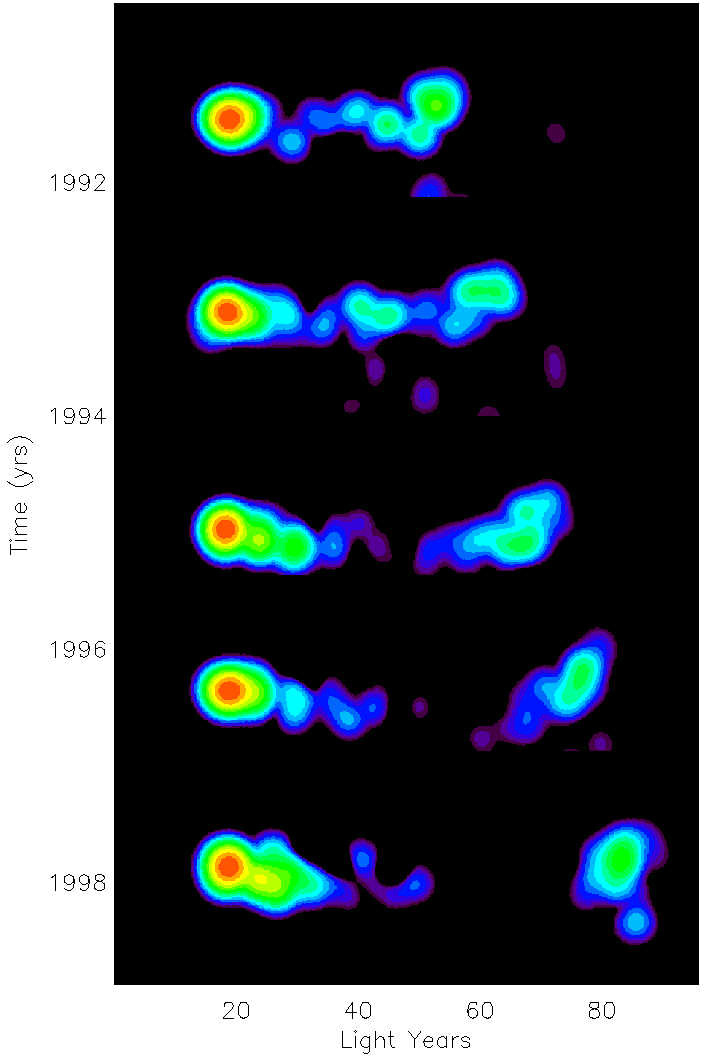
\includegraphics[width=0.8\textwidth]{3c279_mosaic_hi.jpg}
        %\label{fig:}
    \end{minipage}%
    \hfill
    \begin{minipage}{.4\textwidth}
        \caption{
            % The original document says Quasar IRAS 17596+4221, but I haven’t found any evidence that those are the same objects
            Apparent Superluminal Motion in 3C~279, VLA (\SI{1.2}{\cm}), 1998.
            Image courtesy of NRAO/AUI.\vspace{1ex}\\
            Superluminal motion in quasar 3C~279 is shown in a “movie” mosaic of
            five radio images made over seven years. The stationary core is the
            bright red spot to the left of each image. The observed location of
            the rightmost blue-green blob moved about 25 light years from 1991
            to 1998, hence the changes appear to an observer to be faster than
            the speed of light or “superluminal”. The motion is not really
            faster than light, the measured speed is due to light-travel-time
            effects for a source moving near the speed of light almost directly
            toward the observer. The blue-green blob is part of a jet pointing
            within 2 degrees to our line of sight, and moving at a true speed
            of 0.997 times the speed of light. These five images are part of a
            larger set of twenty-eight images made with the VLBA and other
            radio telescopes from 1991 to 1997 to study the detailed properties
            of this energetic quasar.
        }
    \end{minipage}
\end{figure}

\begin{figure}[!ht]
    \centering
    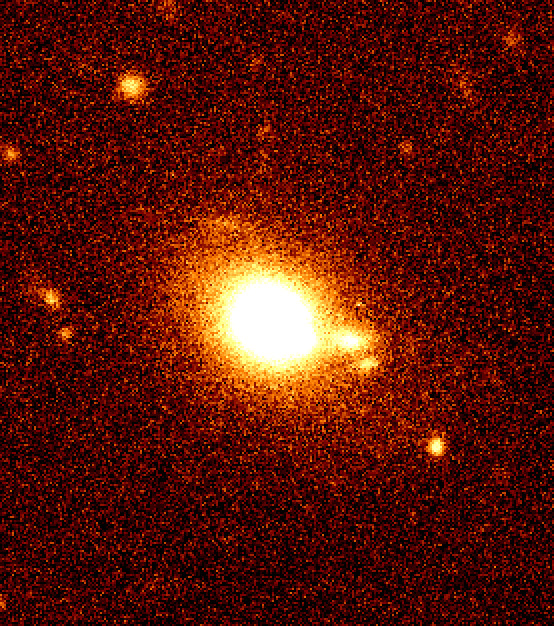
\includegraphics[width=0.5\textwidth]{H0323bl2.jpg}
    %\label{fig:}
    \caption{
        The BL Lac object H~0323+022 ($z=0.147$) imaged at ESO NTT (R
        filter). The host galaxy and close companions are visible.
        \FIXME{Missing a part of the figure}
    }
\end{figure}

\begin{figure}[!ht]
    \noindent
    \begin{subfigure}[t]{.495\textwidth}
        %\includegraphics[width=\textwidth]{}
        %\label{fig:}
        %\caption{
        %}
        \FIXME{Missing figure}
    \end{subfigure}%
    \hfill
    \begin{subfigure}[t]{.495\textwidth}
        %\includegraphics[width=\textwidth]{}
        %\label{fig:}
        %\caption{
        %}
        \FIXME{Missing figure}
    \end{subfigure}
    \caption{
        The figure on the left shows a typical BL Lac with high variability and
        broad band spectra. It requires a coordinated HE and multi-lambda
        monitoring to constrain the SED and its evolution. Similarly, details
        of the various parts in the spectra of the 3C~279 quasar are on the
        right.
    }
\end{figure}

\subsection{Young Stellar Objects}

\subsubsection{Definition}

A \textbf{pre-main sequence star} (PMS star or PMS object) is a star that has
not yet reached the main sequence. In the following we shall consider mainly
loss mass stars with mass less or equal to two solar masses. High mass pre-main
sequence star exhibits strong outflows and winds but not well structure jets at
least at the present stage of observations. Loss mass stars go through the
stage of T-Tauri star or FU Orionis star ($<\SI{2}{\Msun}$). High mass stars
are usually Herbig Ae/Be stars (\SIrange{2}{8}{\Msun}).

\subsubsection{\texorpdfstring{HH objects and $CO$ Outflows}{HH objects and CO Outflows}}

Jets in YSOs where first seen through HH objects. They were defined as bright
knots initially. Usually aligned along a given axis. With the development of
new instruments (in particular the HST), they appear as complex structure and
often internal shocks or bow shocks. Bow shocks are characterized by the
C-Shock front as seen on the extremity of HH34 below (right).

In HH34 (and many other HH objects), the evolution seen from various successive
observations allows to measure proper motion of the knots. Typical values of a
few hundreds of km/s are usually inferred. However some knots may be standing
shocks and the proper motion of the shocks is not directly the speed of the
underlying jets though similar velocities are measured by other means.

These premain stars have accretion-ejection systems with typical accretion
rates of $\dot{M}_\mathrm{accr}=\SIrangeto{e-7}{e-6}{\Msun\per\yr}$. Around
\SI{30}{\percent} of these objects also have jets with typical wind mass loss
rates of $\dot{M}_\mathrm{jet}=\SIrangeto{e-8}{e-7}{\Msun\per\yr}$, densities
$n_\mathrm{jet}=\SIrangeto{e3}{e7}{\per\cubic\cm}$ (this is strongly model
dependent) and temperatures around $\SIrangeto{e3}{e4}{\kelvin}$. Of course the
density in the accretion disk is much higher and the temperature much lower.

\subsubsection{\texorpdfstring{Molecular flows $H_2$, $CO$}{Molecular flows H2, CO}}

Next picture of the HST is called “Birth and death of the Milky Way”. It shows
a multi-wavelength picture with dark clouds illuminated and ionized by stars.
Clouds are clumps resulting from the Parker \FIXME{Jeans?} instability in the
Milky Way. They are themselves unstable and because of gravitational collapse
they contract forming accretion torii and disks.

Some disks (seen in infra red, red contours in next figure) show very powerful
molecular outflows sometimes associated with the previous HH objects and
Optical jets but not always. Molecular outflows with mass loss rates of
$\dot{M}_\mathrm{jet}=\SI{e-5}{\Msun\per\yr}$, velocity a few 10 km/s and cold
temperatures of a tens of Kelvin. The underlying accretion disks have accretion
rates higher than typically $\dot{M}_\mathrm{accr}=\SI{e-4}{\Msun\per\yr}$.

HH211: Another nice example of a powerful molecular outflow with its inner
accretion disk. Note that the inner structure is not very different from some
pictures of Planetary Nebulae.

Molecular outflows are collimated in the observational perspective but not as
well as optical jets. From a theoretical point of view the opening angle is so
large that they may be considered as uncollimated winds. The opening angle is
the angle the outflow makes from its central source. They are usually
surrounding the optical jet when there is one.

\subsubsection{Accretion in YSOs}

The accretion process is always present even if outflows are not. This means
either that the ejection is episodic or (more likely) that accretion does not
necessarily require all the time the formation of a collimated source.

Before having disk images, the presence of an accretion disk was deduced from
the infrared excess measured by the Spectral Index.

\[
    \text{Spectral Index:}\quad \alpha=\frac{\d{\log(\nu F)}}{\d{
    \log(\nu)}}\quad\text{where}\quad F_{\nu}\quad\text{is the flux density.}
\]

\FIXME{$F_\nu$ instead of $\nu F$ maybe?}

For disks in YSO, the spectral index is calculated in the wavelength interval
of \SIrange{2.2}{10}{\um} (near infrared region).

In 1986 Lada C.J. and Wilking B.A. were the first to established the existence
of various classes now known as Class I,II,III. \cite{1993ApJ...406..122A}
discovered a younger class called class 0, with a strong sub-millimeter
emission, but very faint at $\lambda<\SI{10}{\um}$. In summary the classes are:
\begin{itemize}
    \item \textbf{Class 0} sources: undetectable at $\lambda<\SI{10}{\um}$
    \item \textbf{Class I} sources: $\alpha>0.3$
    \item \textbf{Flat spectrum} sources: $0.3>\alpha>-0.3$
    \item \textbf{Class II} sources: $-0.3>\alpha>-1.6$
    \item \textbf{Class III} sources: $\alpha<-1.6$
\end{itemize}

The following figure gives a schematic view of the spectrum and the role of the
accretion disk (from André, 1996).

\FIXME{Make all the references proper ones}

More information on accretion disks is expected from next generation of
instruments like ALMA and Herschell (HIFI).

\subsection{Need for Accretion, Eddington Luminosity}

\subsubsection{Luminosity: Only gravity can do it}

Why do we need to have accretion? After all the equilibrium of disk does not
need any accretion, it could rapidly be under the action of the centrifugal
force.

Accretion,
\begin{itemize}
    \item allows to increase the mass of the central object, either black hole
          or super massive black hole in AGN, or Young Stars. This is of course
          an essential ingredient in the process of star formation and Active
          Galactic Nuclei formation.
    \item is a way to convert gravitational energy into radiation. This was the
          first argument to invoke accretion in the context of cataclysmic
          variables.
    \item is a way to redistribute angular momentum:
          \begin{itemize}
              \item either because of viscosity. This is thought to be the case
                    in low magnetization disk where there is no outflow. The
                    low magnetization also favors MRI magneto rotational
                    instabilities and thus the presence of highly turbulent
                    accretion.
              \item or because it induces a strong outflow. This would be the
                    case for highly magnetized disk where the
                    magnetocentrifugal driving can eject plasma. Magnetic
                    diffusivity is still needed however.
          \end{itemize}
    \item is a way to brake the central star. The braking of the central star
          was though to occur through the magnetosphere connection between the
          star and the disk. This is the so-called disk locking. In the case of
          YSO, it turns out to be inefficient and stellar winds are needed.
\end{itemize}

In order to quantify accretion we can estimate the specific available energy.
It corresponds to the free fall energy:
\begin{equation*}
    \frac{E}{m} \approx \frac{GM_*}{R}
\end{equation*}

The available power is:
\begin{align*}
    P & = \frac{\d{E}}{\d{t}} \approx \frac{GM_*}{R} \frac{\d{m}}{\d{t}} = \frac{GM_*}{R} \dot{M}_\mathrm{acc} \\
      & \approx \num{e38} \left(\frac{\dot{M}_\mathrm{acc}}{\SI{e18}{\g\per\s}}\right) \left(\frac{M}{\SI{2e33}{\g}}\right) \left(\frac{\SI{7e10}{\cm}}{R}\right) \si{\erg\per\s} \\
      & \approx \num{e38} \left(\frac{\dot{M}_\mathrm{acc}}{\SI{e-8}{\Msun\per\yr}}\right) \left(\frac{M}{\si{\Msun}}\right) \left(\frac{\si{\Rsun}}{R}\right) \si{\erg\per\s}
\end{align*}
with
\begin{align*}
    \si{\Msun} &= \SI{2e33}{\g} \\
    \si{\Rsun} &= \SI{7e10}{\cm} \\
    R_\mathrm{NS}   &= \SI{10}{\km} = \SI{e6}{\cm} = \SI{e-4}{\Rsun}
\end{align*}

Thus the available power depends on the accretion rate and the compactness M/R.
The efficiency is the conversion rate,
\begin{equation*}
    \frac{\d{E}}{\d{t}} = \varepsilon \dot{M} c^{2} \Rightarrow \varepsilon = \frac{GM_*}{c^{2}R}
\end{equation*}

In the Newtonian regime, we obtain an efficiency of $\varepsilon = 0.15$ for an
object with a radius of \SI{10}{km}, \SI{1}{\Msun}, typical for a neutron star
or a non rotating galactic black hole.

In the relativistic regime for a black hole in maximum rotation we have a
larger range of efficiency $\varepsilon \approx \numrange{0.059}{0.42}$.

We can compare the efficiency in various fields in Physics :
\begin{itemize}
    \item In Chemistry the typical energy is $\approx \SI{13}{\electronvolt}$,
          energy of ionization, therefore $\varepsilon < 10^{-8}$ thus
          \begin{equation*}
              \frac{\d{E}}{\d{t}} \approx \frac{\SI{1}{\electronvolt}}{m_p c^2} m_p c^2 \dot{M}
          \end{equation*}
    \item In nuclear fusion $\approx \SI{1}{\mega\electronvolt}$, $4H \rightarrow He$ , $\varepsilon < 10^{-2}$
          \begin{equation*}
              \frac{\Delta E_{4 \mathrm{H} \rightarrow \mathrm{He}}}{m c^2} \approx \frac{4 m_\mathrm{H} - m_\mathrm{He}}{4 m_\mathrm{H} c^2} c^2 \dot{M}
          \end{equation*}
\end{itemize}

Accretion is ten times more efficient per mass unit to convert energy with a
compact object.
\begin{itemize}
    \item If it is a galactic Black Hole we get
          \begin{align*}
              R_\mathrm{S} &=\frac{2 G M_\mathrm{BH}}{c^2} = \SI{3}{\km} \\
              \frac{M_\mathrm{BH}}{R_\mathrm{S}} &= 10^5 \frac{\si{\Msun}}{\si{\Rsun}}, \quad \varepsilon = 0.5
          \end{align*}
    \item This is similar for a Neutron Star
    \item For a Supermassive Black Hole the compactness and the efficiency are
          identical, only the radius differs
          \begin{equation*}
              R_\mathrm{S} =\frac{2 G M_\mathrm{BH}}{c^2} = \SIrange{3e11}{e14}{\cm}
          \end{equation*}
    \item For a White Dwarf
          \begin{equation*}
              \frac{M_\mathrm{WD}}{R_\mathrm{WD}} = 10^2 \frac{\si{\Msun}}{\si{\Rsun}}, \quad M_\mathrm{WD} = \si{\Msun}, \quad R_\mathrm{WD} = \SI{e-2}{\Rsun} = \SI{e9}{\cm}
          \end{equation*}
    \item For a Young Star
          \begin{equation*}
              \frac{M_\mathrm{YSO}}{R_\mathrm{YSO}} \approx \frac{\si{\Msun}}{\si{\Rsun}}, \quad M_\mathrm{YSO} = \si{\Msun}, \quad R_\mathrm{YSO} = \SI{2}{\Rsun} = \SI{2e11}{\cm}
          \end{equation*}
    \item For Jupiter
          \begin{equation*}
              \frac{M_J}{R_J} = 10^{-2} \frac{\si{\Msun}}{\si{\Rsun}}, \quad M_\mathrm{J} = \SI{e-3}{\Msun}, \quad R_J = \SI{0.1}{\Rsun} = \SI{e10}{\cm}
          \end{equation*}
\end{itemize}

\subsubsection{Eddington Luminosity}

We can define the Eddington luminosity, assuming isotropy and equilibrium
between radiative pressure and gravity:
\begin{align*}
    F_\mathrm{grav} & = F_\mathrm{rad} \\
    \frac{G M m_p}{R^2} &= P_\mathrm{rad}\sigma_{T,\gamma/e^-} \\
                        &= \frac{u_\mathrm{rad}}{3}\sigma_T \\
                        &= \frac{1}{3}\frac{L R}{\frac{4}{3}\pi R^3 c}\sigma_T\\
    \frac{G M m_p}{R^2} &= \frac{L\sigma_T}{4\pi R^2 c}
\end{align*}

\fxnote{Missing picture}

We can rewrite the gravitational force:
\begin{equation*}
    F_\mathrm{grav} = \frac{G M m_p}{R^2} = F_\mathrm{rad} = \sigma_T \frac{L}{4 \pi R^2}\frac{1}{c}
\end{equation*}

Thus, it defines a luminosity called \emph{Eddington Luminosity} where the
radiative pressure gradient equals the gravitational force:
\begin{align}
    L_\mathrm{Edd} &\approx \num{e33} \left( \frac{M}{\si{\Msun}} \right) \si{\erg\per\s} \\
    \dot{M}_\mathrm{Edd} &\approx \num{e18} \left( \frac{\varepsilon}{0.1} \right) \left( \frac{M}{\si{\Msun}} \right) \si{\g\per\s} = \SI{e-8}{\Msun\per\yr}
\end{align}

\subsubsection{The disk spectrum}

Gas heating implies a balance between matter and radiation. This can be
expressed under the form of a black body such that:
\begin{equation}
    \frac{\d E}{\d t} = \frac{GM_\star}{R}\dot{M}_\mathrm{acc} = 4\pi R^2\sigma T^4
\end{equation}

and the effective temperature of the equivalent black body is given by:
\begin{align}
    k_b T_\mathrm{bb} & \approx \SI{2}{keV} \left( \frac{\dot{M}}{\SI{e-8}{M\per\yr}} \right)^{\nicefrac{1}{4}} \left( \frac{M}{M_\odot} \right)^{\nicefrac{1}{4}} \left( \frac{R}{\SI{e-4} R_\odot} \right)^{-\nicefrac{3}{4}} \\
    k_b T_\mathrm{bb} & \approx \SI{1.5}{keV} \left( \frac{L_\mathrm{Edd}}{\SI{e38}{\erg\per\s}} \right)^{\nicefrac{1}{4}} \left( \frac{R}{\SI{e6}{\cm}} \right)^{-\nicefrac{1}{2}}
\end{align}

Then if all the radiation is converted into energy:
\begin{align}
    \frac{3}{2}\dot{M}\frac{k_b T_\mathrm{bb}}{\mu m_H} & \approx \frac{GM_\star}{R}\dot{M_\mathrm{acc}}
\end{align}

\begin{equation}
    \tcboxmath{
        \begin{aligned}
            \frac{3}{2}k_bT_\mathrm{bb} & \approx \mu m_H \frac{GM_\star}{R} \\
                                        & \approx \num{90} \left( \frac{M}{M_\odot} \right) \left( \frac{R}{\SI{e6}{cm}} \right)^{-1} \si{MeV}
        \end{aligned}
    }
\end{equation}

\fxnote{it is highlighted in the original text}

We get for:
\begin{itemize}
    \item \textbf{a galactic black hole}
        \begin{equation}
            \SI{2}{keV}\left( \frac{\dot{M}}{\SI{e-8}{M_\odot\per\year}} \right)^{\nicefrac{1}{4}} \left( \frac{M}{M_\odot} \right)^{\nicefrac{1}{4}} \left( \frac{R}{\SI{e-4}{R_\odot}} \right)^{-\nicefrac{3}{4}} < kT < \SI{90}{MeV}\left( \frac{M}{M_\odot} \right)^{\nicefrac{1}{4}} \left( \frac{R}{\SI{e-4}{R_\odot}} \right)^{-1}
        \end{equation}
        For a mass loss rate of $\dot{M} = \SI{e-8}{M_\odot\per\year}$, the
        spectrum spans from soft X to gamma rays.
    \item \textbf{a white dwarf}
        \begin{equation}
            \SI{10}{eV} < kT < \SI{45}{keV}
        \end{equation}
        The spectrum is from $\SI{1000}{\angstrom}$ to hard X rays.
    \item \textbf{a $\SI{e8}{M_\odot}$ super-massive black hole} and an
          accretion rate $\dot{M} = 0.1-\SI{1}{M_\odot\per\yr}$,
          \begin{equation}
              \SI{20}{eV} < kT < \SI{90}{MeV}
          \end{equation}
          The spectrum is from UV to gamma, softer than stellar BHs
    \item \textbf{a young low mass star} $M = M_\odot$, a mass loss rate of
          $\SIrange{e-7}{e-6}{M_\odot\per\year}$, the radiation spans:
          \begin{equation}
              0.3-\SI{3}{eV} < kT < \SI{4.5}{keV}
          \end{equation}
          corresponding to radiations from IR, visible to X rays.
    \item \textbf{a Jupiter}, the range is
          \begin{equation}
              \SI{e-3}{eV} < kT < \SI{5}{eV}
          \end{equation}
          from far IR to optical
\end{itemize}

As a matter of fact the range of spectrum we just deduced coincides with the
observed spectrum for accretion disks around these objects.

\subsubsection{AGN Luminosity and Spectra}

The luminosity observed in AGNs is of the order of $\SI{e46}{\erg\per\s}$. If
the total luminosity is lower than the Eddington luminosity, which is
reasonable, the mass of the central black hole has to be larger than $M >
\SI{e8}{M_\odot}$.

The luminosity could be due to nuclear reactions, if we have a large population
of star burst. This implies a burst rate of $\dot{M} \sim
\SI{10}{M_\odot\per\yr}$. Considering that the galaxy has $M_\mathrm{galaxy}
\sim \SI{e11}{M_\odot} \sim \SI{e11}{stars}$, it would be emptied in 10 billion
years. This is too short and excludes the scenario of AGN being star burst
galaxies.

Conversely, if the luminosity is due to accretion, the accretion rate required
is $\dot{M} \sim \si{M_\odot\per\yr}$. The mass luminosity ratio is $M/L \sim
10$. Thus the luminosity of a standard galaxy is $L_\mathrm{galaxy} \sim
\SI{e43}{\erg\per\s}$ and the luminosity of a quasar is a thousand times
higher: $L_\mathrm{quasar}\sim 1000 L_\mathrm{galaxy}$. \textbf{For Seyfert
galaxies, the luminosity is typically around $\SIrange{e43}{e45}{\erg\per\s}$
while for quasars it is between $\SIrange{e45}{e48}{\erg\per\s}$}.

The observed variability is typically of one week $\Delta t \sim \SI{6e5}{s}$.
Considering that the speed of light is the upper speed limit, the causality
principle implies that the emission region cannot be larger than $R \leq
c\Delta t \sim \SI{2e16}{cm} \sim \SI{0.01}{pc}$. This means that the emission
comes from a very narrow region with a rather high density. To satisfy this, it
is difficult to have stellar clusters (e.g. Sgr A :
$\SI{4e16}{M_\odot\per\pc^3}$).

The figure bellow \fxnote{put the figure} displays a typical \textbf{BL Lac
Spectral Distribution}. \textbf{BL Lac} are typical radio loud AGNs. Nowadays,
we have a good knowledge of the multi-wavelength spectrum from radio to gamma
rays.

\textbf{Seyfert and Quasar Spectral Distributions} are quite similar to BL Lac.
Each component is explained by the composition of the disk and the jet. The
central BH is surrounded by a cold accretion disk of gas and dust. On top of
the disk, close to the central object, a hot corona must be present. The radio
levels depend on the presence or of a central jet.  \fxnote{Missing figure
here}

The cascade model explains how the different frequencies are emitted and how
they are correlated in space and time as shown in the following figure.
\fxnote{missing figure here}

\subsection{Need for Jets}

\subsubsection{Energy in the extended lobes}

In radio loud galaxies and quasars, an extended emission into the lobes is
observed. Such galaxies are at cosmological distances, typically
$\SI{200}{\Mpc}$. As $d\sim z\frac{c }{H}$, we have a redshift of $z\sim 0.05$.

Considering that the lobe size is of the order of magnitude
$d_\mathrm{lobe}\sim \SI{100}{\kpc}$, for a plasma that moves in the at speed
$v\sim \SI{e8}{\cm\per\s} = \SI{1000}{\km\per\s}$, the time delay necessary to
reach the lobe is $\Delta t_\mathrm{life} \sim
\frac{\num{e5}\times\num{3e18}}{\num{e8}} \si{Myr} \sim \SI{100}{Myr}$. The
observed luminosity begin $\SI{e44}{\erg\per\s}$ at $\SI{e9}{\Hz}$, the amount
of total energy is huge and equal to $\num{e44}\times\SI{3e15}{\erg} \sim
\SI{e60}{\erg}$. This is equivalent to $\SI{e6}{M_\odot}$.

We observe radio emission both in extended and compact sources. In extended
sources, the radio spectrum goes like $F_v \sim v^{-0.5} \textrm{ or } v^{-1}$,
while in compact sources it is $F_v \sim \mathrm{cst}$. The nature of the
emission is not obvious and was in question for sometimes \fxnote{not really
English there}:
\begin{itemize}
    \item Thermal emission was immediately excluded for the radio component as
          it would have implied too high temperatures
    \item \emph{Bremstrahlung} emission could have been a reasonable candidate,
          but because of absorption, one expects this process to be limited.
    \item The observed high polarization could be the signature of a Compton
          emission but this would imply an extremely low temperature $T <
          \SI{3}{K}$.
\end{itemize}

Finally it turned out that \textbf{synchrotron} emission was the best candidate
to explain the radio excess and the slope of the spectral emission.

\subsubsection{Synchrotron emission}

The total energy density in the lobes is
\begin{equation}
    U \sim \frac{10^{60}}{10^{69}} \approx \SI{e-9}{\erg\per\s}
\end{equation}

If we make a hypothesis of equipartition, which is completely arbitrary in the
case of jets but the simplest assumption one can make, then $\frac{B^2}{8\pi}
\sim \SI{e-9}{\erg\per\cm\cubed}$ and therefore $B \sim \SI{100}{\micro G}$.
The synchrotron frequency is given by $\nu = \num{4.3e6} B\gamma^2 \sin\alpha\
\si{\Hz}$. At \SI{46}{Hz}, we have a Lorentz factors of $\gamma \sim
\numrange{e3}{e4}$. This means that the synchrotron emission comes from
relativistic electrons. The cooling time is of the order of \SI{1}{Myr}, which
is much less than the life time. It has several consequences on the emission
region:
\begin{itemize}
    \item there must be an \emph{in situ} continuous production of highly
          relativistic electrons
    \item only a jet can inject matter so far from the central core
    \item there are shocks where electrons are re-accelerated
\end{itemize}

A large fraction of the total energy is not visible and must be in the form of
kinetic energy. Only a jet that feeds the lobe can provide this energy, even if
it is not visible.

\subsubsection{Proper motion}

Proper motion of knots is now measured in all the objects. These are the motion
of the shocks so probably an underestimation of the jet speed itself.
Nevertheless, the velocity is much higher than the local sonic speed and only
jets can explain supersonic speeds. Typical values in YSO jets are a few
hundreds of \si{\km\per\s}.

\fxnote{Missing figure of proper motion}

In AGN jets, we see apparent superluminal motions that can be explained only if
the shocks and the jets are moving at (nearly) the speed of light. Superluminal
motions are also observed in microquasars.

\fxnote{VLBA image + GRS 1915}

\subsection{Rotation and the Angular Momentum transfer}

\subsubsection{The Angular Momentum problems in YSO}

The biggest obstacle to the formation of stars from diffuse gas is that a star
can contain only a tiny fraction (less than \SI{e18}{\square\cm\per\s}) of the
initial angular momentum of the gas from which it formed
(\SI{e23}{\square\cm\per\s} for a molecular cloud of scale \SI{1}{\pc},
\SI{e21}{\square\cm\per\s} for a dense core of scale \SI{0.1}{\pc}), so that
nearly all of this angular momentum must be removed or redistributed during the
formation process. The angular momentum from the cloud can be removed by
ambipolar diffusion. Yet the problem to go from the core to the star remains.

The specific angular momentum of typical star-forming molecular clouds are at
least three orders of magnitude larger than the maximum speed at the equatorial
plane of the star where the centrifugal force equals gravity. Thus, if we
equals the centrifugal force per unit mass and gravity, we get
\begin{equation}
    \frac{v^2_\textrm{break up}}{R_\star} = \frac{GM_\star}{R_\star^2}
    \Rightarrow v_\textrm{break up} = R_\star \Omega_\textrm{break up} = \sqrt{\frac{GM_\star}{R_\star}}
    \Rightarrow \Omega_\textrm{break up} = \sqrt{\frac{GM_\star}{R_\star^3}}
\end{equation}

For a typical T Tauri star, the break up value is one to a few hundreds
\si{\km\per\s} while those stars rotate at around \SIrange{5}{20}{\km\per\s}.
The stellar rotation is an order of magnitude bellow the break up velocity.

Here are some recent \textbf{Kepler} mission measurements of rotation in
clusters.  \fxnote{Missing figure} These results can be compared to Bouvier et
al. (\FIXME{Make a ref of that}) results hereafter, showing plots of the
evolution of the rotation as a function of time for Fast Rotators (blue lines)
and Slow Rotators (red lines). The envelope velocity is always slower than the
core velocity. The circle on the right is the position of our Sun. The curves
correspond to evolutionary tracks and are model dependent.

\fxnote{Missing plots}

In the case of a Keplerian disk, to the first order, the centrifugal force
balances gravity $\rho \frac{v_\phi^2}{r} \approx \rho \frac{GM_\star}{r^2}$.
Thus, similarly to the break up velocity we get the Keplerian velocity and
angular frequency:
\begin{equation}
    v_\phi = \sqrt{\frac{GM_\star}{r}}, \quad \Omega = \frac{v_\phi}{r} = \sqrt{\frac{GM_\star}{r^3}}
\end{equation}
\fxnote{Missing scheme}

If the disk edge is connected onto the star as on the above scheme, they should
rotate at the same speed on the boundary layer and the star should thus rotate
at its breakup velocity. As this is not the case, it is obvious that the star
cannot be directly connected to the disk and that some mechanism should exist
to evacuate the angular momentum. One solution to this problem is the
disk-locking mechanism, where the angular momentum of the star is transferred
to the disk \emph{via} the magnetosphere and then the viscosity of the disk
removes the excess of angular momentum. Another solution is that the stellar
wind itself carries away angular momentum while being braked by the magnetic
field.

\subsubsection{Rotation of AGN and Microquasar Central Black Hole}

The problem of the transfer of angular momentum to the black hole in the
accretion disk is similar to the one in YSO. All black holes are surely not
maximally rotating, for instance the Galactic Black Hole of the disk luminosity
shown on next figure is rotating at 0.6 its maximum angular velocity.

If the mass of a Kerr black hole is $M$, its angular momentum $J$, its
Schwarzschild radius is
\begin{equation}
    R_s = \frac{2GM}{c^2}
\end{equation}
and the radius of the horizon is:
\begin{equation}
    R_\mathrm{Kerr} = \frac{Rs}{2} \left( 1 + \sqrt{1-\left( \frac{Jc}{GM^2} \right)^2 } \right)
\end{equation}

The angular momentum cannot be higher than the value that makes the square root
negative, so
\begin{equation}
    J < J_\mathrm{max} = \frac{GM^2}{c} = MR_\mathrm{Kerr}c
\end{equation}

We define the rotation parameter as:
\begin{equation}
    \alpha = \frac{J}{J_\mathrm{max}} < 1
\end{equation}

How do we know the nature of the central black hole in AGNs? The main clue
comes from the iron-K line which can be explained only with a central rotating
black hole.

\fxnote{Missing figure}

The red component of the line is the signature of general relativity effects
due to the BH. It is explained by the gravitational redshift (Einstein effect)
in addition to special-relativity Doppler shift and beaming, as shown on the
following figure of a synthetic Iron K Line produced by a rotating accretion
disk around a BH.

\fxnote{Missing figure}

The line profile can be modeled using a Schwarzschild BH or a non rotating BH
(below left). The discrepancies can be reduced by keeping the Schwarzschild BH,
but taking into account the reflected continuum (below right).

\fxnote{Missing figure}

However, it seems the best fit is obtained by considering a rotating BH, or
Kerr BH in maximal rotation.

The last figure is generated for a maximally rotating Kerr BH. Note the absence
of the dotted line on the right part.

\subsubsection{Conclusion, The Global Picture of the Jet}

In conclusion, the system we have is a rotating disk and a central object. The
plasma is ionized. We have all the ingredients to have a complex structure
involving rotation and magnetic field.

\section{Thermal Accretion and Winds}

Because of rotation and magnetic fields, accretion and ejection are
3-dimensional and close to axisymmetry. However, some of the basic features can
be under understood by looking a 1-dimensional processes and especially
spherically-symmetric accretion and wind.

\subsection{Spherical Accretion and Wind}

\subsubsection{Bondi Accretion}

Let's consider an ideal fluid around a star in-falling (accretion), with a
spherical symmetry. Using spherical coordinates $(r,\theta,\phi)$ we write the
physical variables describing the fluid:
\begin{equation}
    \rho = \rho(r),\quad P = P(r), \quad \vv{v} = \vv{v}(r)
\end{equation}

The conservation of energy gives:
\begin{equation}
    E = \frac{1}{2}v^2 + h + \Phi_\mathrm{grav}
\end{equation}

For the sake of simplicity, let's assume the flow is isothermal. The
gravitational potential is
\begin{equation}
    \Phi_\mathrm{grav} = - \frac{GM_\star}{r},\quad \textrm{$M_\star$ is the mass of the star}
\end{equation}
and the enthalpy is:
\begin{equation}
    h = \int \frac{\d p}{\rho} = c_s^2 \ln \rho
\end{equation}
because the flow is isothermal. Here, $c_s^2 = 2 \frac{k_b T}{m_H}$ is the
sound speed.

The conservation equations are written as follow:
\begin{equation}
    \tcboxmath{
        \begin{aligned}
            \vv{\nabla}\cdot \left( \rho\vv{v} \right) = 0, \quad& \textrm{Mass conservation}\\
            \rho v \frac{\d v}{\d r} = -\frac{\d p }{\d r} - \rho \frac{GM_\star}{r^2},\quad & \textrm{Euler equation}\\
            p = c_s^2 \rho,\quad & \textrm{Equation of state}
        \end{aligned}
    }
\end{equation}
The mass conservation equation gives:
\begin{equation}
    \rho v r^2 = \textrm{constant} = \dot{m}, \quad \textrm{$\dot{M}$ is the accretion rate and $\dot{m}=\dot{M}/4\pi$}
\end{equation}

Rewriting the energy, we get :
\begin{align}
    E &= \frac{1}{2}v^2 + c_s^2 \ln \frac{\dot{m}}{vr^2} - \frac{GM}{r} \\
      &= \frac{c_s^2}{2}\left[ \frac{v^2}{c_s^2} + 2\ln \frac{\dot{m}}{vr^2} - \frac{2GM}{c_s^2r}\right] \\
      &= \frac{c_s^2}{2} \left[\frac{v^2}{c_s^2} + \ln \frac{c_s^2}{v^2} + 4\ln \frac{2GM}{c_s^2r} - \frac{2GM}{c_s^2r} + 2\ln \frac{\dot{m}c_s}{(2GM)^2} + 2\ln c_s^2\right]
\end{align}

Let $r_c = \frac{GM}{2c_s^2}$. The Bernoulli constant gives that the
solutions are given implicitly by drawing the following isocontours:
\begin{equation}
    \tcboxmath{
        \left( \frac{v}{c_s} \right)^2 - \ln \left( \frac{v}{c_s} \right)^2 - 4\ln \frac{r}{r_c} - 4 \frac{r_c }{r} = C
    }
\end{equation}
where $C$ is a constant.

By deriving this equation or directly from Euler equation,
\begin{align}
    \rho v \frac{\d v}{\d r}  &= -c_s^2 \frac{\d \rho}{\d r} - \rho \frac{GM}{r^2} \\
    r \frac{v}{c_s^2} \frac{\d v}{\d r} &= \underbrace{-\frac{r}{\rho}\frac{\d \rho}{\d r}}_\textrm{mass conservation} - \frac{GM}{c_s^2r} \\
                            &= r \left( \frac{2}{r} + \frac{c_s}{v} \frac{\d(v/c_s)}{\d r} \right) - \frac{2r_c }{r} \\
    \frac{r}{r_c }\frac{v}{c_s }\frac{\d (v/c_s)}{\d (r/r_c)} & = \frac{r}{r_c} \left( \frac{2r_c }{r} + \frac{c_s}{v} \frac{\d(v/c_s)}{\d(r/r_c )} \right) - \frac{2r_c }{r}
\end{align}

\begin{equation}
    \label{eq:speed_eq}
    \tcboxmath{
        \left( \frac{v}{c_s} - \frac{c_s}{v} \right) \frac{\d \left( \frac{v}{c_s} \right) }{\d \left( \frac{r}{r_c } \right) } = 2 \frac{r_c}{r} \left( 1 - \frac{r_c }{r} \right)
    }
\end{equation}

The set of solutions of the previous equation is displayed on the two following
figures. This is the topology of the solutions.

We note $M = \frac{v}{c_s}$ the Mach number.

We could show that for polytropic winds ($p = Kp^\gamma$), the topology of the
Mach number doesn't change even though the sound speed is no longer a constant
but depends on distance:
\begin{equation}
    c_s^2 = \frac{\d p}{\d \rho}
\end{equation}

A few years before Parker, \cite{1952MNRAS.112..195B} proposed that accretion
onto a star or a black hole could become supersonic. This corresponds to one of
the 2 critical solutions. Of course, supersonic accretion onto the star ends by
a shock, which explains X-ray emissions of cataclysmic binaries.

We can calculate for this solution the mass accretion rate, which is by
definition
\begin{equation}
    \dot{M} = 4\pi r^2 \rho (-v) = 4\pi r_c^2 \rho_s c_s
\end{equation}

Evaluating the energy at the critical point:
\begin{equation}
    E = \textrm{constant} = \frac{1}{2}v^2 + c_s^2 \ln\rho - \frac{GM}{r} = \frac{1}{2}c_s^2 + c_s^2 \ln \rho_s - \frac{GM}{r_c}
\end{equation}
we get the velocity both at infinity and close to the star:
\begin{align}
    v^2 &= 2c_s^2 \left( -\frac{3}{2} + \ln \frac{\rho_s}{\rho} \right)  + \frac{2GM}{r} \\
        & \xrightarrow{r\to 0} \frac{2GM}{r} \\
        & \xrightarrow{r\to\infty} 0\ \Rightarrow \rho_S = \rho_\infty e^{\nicefrac{3}{2}}
\end{align}

We see that close to the star, the fluid is in free fall. The mass accretion
rate of the trans-sonic solution is thus:
\begin{equation}
    \dot{M}_\mathrm{transsonic} = \pi \left( GM \right)^2 e^{\nicefrac{3}{2}} \frac{\rho_\infty}{c_s^3}
\end{equation}

\subsubsection{Parker wind or thermally driven outflow}

We now suppose that the ideal fluid around the star is out-flowing (wind). We
assume spherical symmetry. Using the same spherical coordinates ($r, \theta,
\phi$), we can derive the same equations with different boundary conditions.
Here, conditions are given at the stellar surface and not at infinity. Again we
have $\rho = \rho(r)$, $P = P(r)$, $\vv{v} = \vv{v}(r)$.

Even if the fluid is magnetized, the assumption of spherical symmetry implied
that the magnetic field parallel to the stream does not give any contribution.
The Poynting flux is zero.

For the sake of simplicity, we'll assume again that the flow is isothermal. The
original Parker model (\cite{1958ApJ...128..664P}) for the solar wind already
contained all the necessary ingredients; it assumed the flow to be isothermal
close to the sun and adiabatic farther away where the wind is accelerated.

The final set of equation is the same. Basically we solve:
\begin{equation}
    \tcboxmath{
        \left( \frac{v}{c_s} - \frac{c_s}{v} \right) \frac{\d \left( \frac{v}{c_s} \right) }{\d \left( \frac{r}{r_c } \right) } = 2 \frac{r_c}{r} \left( 1 - \frac{r_c }{r} \right)\quad \textrm{or} \quad
        \left( \frac{v}{c_s} \right)^2 - \ln \left( \frac{v}{c_s} \right)^2 - 4\ln \frac{r}{r_c }- 4 \frac{r_c}{r} = C
    }
\end{equation}

The topology of the solutions is the same as previously but with a new
interpretation. We can also plot in 3D the energy versus distance and velocity
to make clear the critical point is sitting on a saddle. We still have $M =
\frac{v}{c_s}$ the Mach number. We see that the r.h.s. of \eqref{eq:speed_eq}
vanishes for $r=r_c$ and the l.h.s. for $v=c_s$ except if the flow has reached
super sonic speed at the critical radius. Thus solutions have an horizontal or
a vertical tangent except for the two critical solutions where there is
\textbf{a fixed or critical point}. This is a \textbf{saddle}
point\footnote{The two slopes of the critical solutions at the critical point
can be determined using l'Hospital's rule, i.e. expanding $\frac{v}{c_s} = 1 +
\delta$ and $\frac{r}{r_c} = 1 + \varepsilon$ to first order. We obtain a
second algebraic equation for the slope $\delta/\varepsilon$ which solutions
are the slopes at the saddle point,
\begin{equation*}
        \frac{\delta}{\varepsilon} = \frac{\d (v/c_s)}{\d (r/r_c)} = \frac{2 \frac{r_c }{r}\left( 1 - \frac{r_c }{r} \right) }{\frac{v}{c_s} - \frac{c_s}{v}} = \frac{2 \frac{1}{1+\varepsilon} \left( 1 - \frac{1}{1+\varepsilon} \right) }{1 + \delta - \frac{1}{1+\delta}} \approx \frac{2(1-\varepsilon)\varepsilon}{1 + \delta - 1 + \delta} \approx \frac{2\varepsilon}{2\delta} \Rightarrow \frac{\delta}{\varepsilon} = \pm 1
\end{equation*}} with two slopes. The saddle nature of the point is better seen
in the 3D plot of the energy in phase space ($r, v$).

\subsubsection{Solar wind (Parker 1958)}

The breeze solutions have zero velocity asymptotically, but the pressure is non
zero and cannot match the interstellar pressure:
\begin{equation}
    v^2 = 2 c_s^2 \left( -\frac{3}{2} + \ln \frac{\rho_s}{\rho} \right) + \frac{2GM}{r} \xrightarrow{r\to\infty} 0\Rightarrow \rho_\infty = \rho_s e^{-\nicefrac{3}{2}} \neq 0 \Rightarrow \rho_\infty \neq 0
\end{equation}

Thus they are very similar in behavior to the static solutions, which we have
shown to be excluded. Parker showed that the only valid solution is the
critical solution that becomes super sonic with zero pressure at infinity. It
has then been confirmed observationnaly. Parker also showed studying the
polytropic wind that acceleration can be obtained only if the polytropic index
is $\gamma < \frac{3}{2}$. $\frac{c_p}{c_s} = \frac{5}{3}$ being the adiabatic
value for a monoatomic gas, this means that the wind exists only because there is
enough extended heating at the base of the solar corona.

There are some breeze solutions with heat conduction, which have zero pressure
at infinity. Thus the debate was really strong during the 60s, until
observations confirmed Parker's theory. Nowadays, the problem has slightly
shifted. In fact for a temperature of one million Kelvin, the speed at the
earth orbit is of the order of \SI{500}{\km\per\s} with this model. From the
measurements of Ulysses spacecraft, we know that this is effectively the speed
of the slow equatorial wind, but this model is not sufficient to explain the
\SI{800}{\km\per\s} of the fast polar wind. Thus, series of models have been
developed which involve sophisticated not-so-well-known coronal heating,
kinetic theories, etc... is still an open debate.

Similarly to the accretion rate, one can calculate the mass loss rate from the
star through the wind:
\begin{align}
    \dot{M} & = 4\pi r^2\rho v = 4\pi r^2_c\rho_sc_s \\
    \dot{M}_\odot & = \SI{e-14}{M_\odot\per\s} \\
    \dot{M}_\mathrm{TTauri} &= \SI{e-8}{M_\odot\per\s}
\end{align}

\subsection{More on 1D models}

\subsubsection{Critical surfaces and Horizons}

The critical point corresponds to sonic waves . The stellar surface losses mass
in a steady way only if the mass flux adapts itself to cross the critical
surface. The sonic waves going upstream will make the ejection to evolve until
it reaches the steady state. This critical surface is analogous to the event
horizon around black holes. Beyond this surface, the wind is unable to
propagate sound waves back to the source.

There is a strong analogy between the sonic surface and apparent horizon in
black holes, except that the sound speed replaces the speed of light. This is
illustrated in the following figures.

\fxnote{Missing figure}

If the star rotates, in addition to the sonic surface/horizon there is also an
acoustic ergosphere.

\subsubsection{De Laval Nozzle}

There is a strong analogy between the Parker wind and a flow through a nozzle.
A nozzle is a pipe with a variable cross section. It has a minimum and this
minimum should coincide with the sonic point to have strong supersonic flow,

\fxnote{Missing Figure}

Mass conservation:

\begin{equation}
    \vv{\nabla}\cdot(\rho\vv{v}) \Rightarrow \int \rho\vv{v}\cdot \d \vv{S} = cst \Rightarrow \rho vS = cst
    \Rightarrow \frac{\d \rho}{\rho} + \frac{\d \nu}{\nu} + \frac{\d S}{S} = 0
\end{equation}

Euler equation:
\begin{equation}
    \rho v \frac{\d v}{\d x} = -\frac{\d p}{\d x}
\end{equation}

Equation of state (energy):
\begin{equation}
    p(x) = c_\mathrm{s}^2\rho(x)
\end{equation}

It follows:
\begin{equation}
    v\frac{\d v}{\d x} = -c_s^2\frac{\d\rho}{\rho \d x} = c_s^2\left(\frac{\d v}{v\d x}+\frac{\d S}{S\d x}\right)
    \Rightarrow \left( v - \frac{c_s^2}{v} \right)\frac{\d v}{\d x} = c_s^2\frac{\d S}{S \d x}
\end{equation}

The flow can be transsonic only if $\frac{\d S}{S\d x} = 0 $ which means that
the cross section has an extremum. It is by default a minimum as at the
entrance of the nozzle on the left, $v<c_s$ and $\frac{\d v}{\d x} > 0$ thus
$\frac{\d S}{\d x} > 0 $. If this minimum exists, to be transsonic the flow
must attain the sound speed at the minimum cross section.

\paragraph{Spherical flow, Parker wind}

For a spherical wind we have:
\begin{equation}
    \left( v - \frac{c_s^2}{v}  \right)\frac{\d v}{\d r} = c_s^2\frac{\d S}{S\d r}
    = \frac{2c_s^2}{r} - \frac{GM}{r^2} \Rightarrow \frac{\d \ln S}{\d r} =
    \frac{2}{r} - \frac{GM}{c_s^2 r2}
    \Rightarrow \ln S = \ln r^2 +\frac{GM}{c_s^2r} + k
\end{equation}

And finally:
\begin{equation}
    \tcboxmath{S = Cr^2 \exp\left(\frac{GM}{c_s^2 r}\right)}
\end{equation}

Gravity plays the role of reducing the effective cross section as the radial
flux tubes expands as $r^2$. There is no real throat just an effect of gravity.

\paragraph{Funnel ans 1D flow}
The analogy has been used to explain jets both in the YSO and the AGN contexts.
The argument is to use the presence of the surrounding thick disk close to the
central object has shaped in the form a funnel.

This is the case of the famous \textbf{ Exhaust Model for AGN Jets} suggested
by Blandford \& Rees 1974 (see correct figure), used also in the Ion Supported
Torus model of jet funnel by Phinney 1999 (see other correct figure).

\fxnote{Missing Figure}

Raga and Canto also used this model in 1989 for YSO, invoking a stellar wind to
make the cavity.

\fxnote{Missing figure}

These models suffer strong flaws. The shape of the funnel is somewhat given and
not the result of a really consistent resolution of the MHD equations. The
strongest argument is however that the throat of the funnel is always too far
from the central object to maintain a very small opening angle for the jet.

This leads us to next chapter and to consider axisymmetric models ans not only
1D solutions.

\subsubsection{Vertical structure of a Thin Keplerian Disk}

\section{Theory of Standard Accretion Disks}

\subsection{Shakura Sunyaev Standard Thin Disk}

\subsubsection{Thin Accretion Disk}

\FIXME{Missing figure}

We assume a thin disk as previously Keplerian to first order where the height
can be neglected. In other words we integrate all equations on an annulus $R$
over the height of the disk $H(R)$. First we write mass conservation,
\begin{equation*}
    \diffp{\rho}{t} + \vv{\nabla}\cdot(\rho \vv{v}) = 0
\end{equation*}

Introducing the surface mass density defined as
\begin{equation*}
    \Sigma = \int_{-H}^H \rho \d{z} \approx 2 \rho H
\end{equation*}

so that $2 \pi R \Sigma$ is the mass density per unit length. Integrating the
mass conservation over H (the integral and the derivative being linear and here
independent operators, they can be inverted),
\begin{align*}
    \int_{-H}^H \left( \diffp{\rho}{t} + \vv{\nabla}\cdot(\rho \vv{v}) \right) = 0 % Not a mistake, just for code readability
    &= \diffp{\int_{-H}^H \rho \d{z}}{t} + \vv{\nabla}\cdot\left( \int_{-H}^H \rho \vv{v} \d{z} \right) \\
    &= \diffp{\int_{-H}^H \rho \d{z}}{t} + \vv{\nabla}\cdot\left( \vv{v} \int_{-H}^H \rho \d{z} \right) \\
    &= \diffp{\Sigma z}{t} + \vv{\nabla}\cdot(\Sigma V_R)
\end{align*}

we get mass conservation on each annulus:
\begin{equation}
    \label{eq:alpha_mass}
    \tcboxmath{
        \diffp{\Sigma}{t} + \frac{1}{R} \diffp{(R \Sigma V_R)}{R} = 0
    }
\end{equation}

We assume quasi-Keplerian rotation $V_\varphi = R \Omega_K = \sqrt{\frac{G
M}{R}}$. In reality rotation is slightly sub-Keplerian to allow accretion.

We then use the Angular Momentum conservation, which comes from the global
momentum equation,
\begin{equation*}
    \rho \diffp{\vv{v}}{t} + \rho (\vv{v}\cdot\vv{\nabla})\vv{v} =
    \rho \vv{g} - \vv{\nabla} p - \vv{\nabla}\cdot\left(\rho \overline{\vv{v'} \otimes \vv{v'}}\right) \quad \text{with} \quad V_\varphi \leq R \Omega_K
\end{equation*}

Momentum equation can be written with a turbulent pressure tensor
\begin{equation*}
    \diffp{}{t}(\rho \vv{v}) + \vv{\nabla}\cdot\left(\rho \vv{v} \otimes \vv{v} + \tens{P}_\mathrm{turb}\right) = \rho \vv{g}
\end{equation*}

\FIXME{Need of a better tensorial notation for Pturb}

with the turbulent pressure being
\begin{align*}
    \tens{P}_\mathrm{turb} &= p_\mathrm{gas} \tens{I} + \rho \overline{\vv{v}' \otimes \vv{v}'} \\
    \left(\overline{\vv{v}' \otimes \vv{v}'}\right)_\mathrm{ij} &= \overline{v_i' v_j'} =
    - \nu_T \left( \diffp{\overline{v_i}}{{x_j}} + \diffp{\overline{v_j}}{{x_i}} \right) \\
    \Leftrightarrow \left(\overline{\vv{v}' \otimes \vv{v}'}\right) &=
    - \nu_T \left(\vv{\nabla} \otimes \vv{v} + \vv{v} \otimes \vv{\nabla}\right)
\end{align*}

\FIXME{Same as above}

The molecular viscosity is completely inefficient and cannot explain the source
of viscosity essential to have accretion,
\begin{equation*}
    \mathfrak{R}_\mathrm{e} = \frac{L^2}{\nu T} = \frac{L V}{\nu} \approx \num{e11}
\end{equation*}

Shakura \& Sunyaev suggested then (1971) that the source of viscosity is
turbulence giving an anomalous coefficient for the viscosity.
\begin{equation*}
    \mathfrak{R}_\mathrm{eT} = \frac{L^2}{\nu_T T} = \frac{L V}{\nu_T} \approx \num{e4}
\end{equation*}

\FIXME{Make it a reference}

To explain this turbulence one needs the disk to develop instabilities. Since
Balbus \& Hawley (1991), the instability most favorable seems to be the
Magneto-Rotational-Instability (MRI hereafter).

\FIXME{Make it a reference}

To get the angular momentum conservation on $\phi$, we can multiply by $\vv{R}
\times$, and integrate over height,
\begin{align*}
    &\int_{-H}^H \vv{R} \times \diffp{}{t}(\rho \vv{v}) \d{z} +
    \int_{-H}^H \vv{R} \times \vv{\nabla} \cdot \left(\rho \vv{v} \otimes \vv{v} + \tens{P}_\mathrm{turb}\right) \d{z} =
    \underbrace{\int_{-H}^H \vv{R} \times \rho \vv{\nabla} \nabla_\mathrm{grav} \d{z}}_{= 0} \\
    &\Rightarrow \diffp{}{t} \int_{-H}^H \vv{R} \times (\rho \vv{v}) \d{z} +
    \vv{\nabla} \cdot \int_{-H}^H \vv{R} \times \left( \rho \vv{v} \otimes \vv{v} \right) \d{z} +
    \underbrace{\int_{-H}^H \vv{R} \times \vv{\nabla} p \d{z}}_{= 0} =
    - \vv{\nabla} \cdot \int_{-H}^H \vv{R} \times \left(\overline{\rho \vv{v}' \otimes \vv{v}'}\right) \d{z}
\end{align*}

See the appendix for the correctness of operators inversion.

\FIXME{Add this appendix, link it}

\begin{equation*}
    \Rightarrow \diffp{}{t} \int_{-H}^H \rho R V_\varphi \d{z} + \frac{1}{R} \diffp{}{R} \left( R \int_{-H}^H R \rho V_R V_\varphi \d{z} \right) =
    \frac{1}{R} \diffp{}{R} \left( R G \right)
\end{equation*}

We get,
\begin{equation*}
    \diffp{\left(\Sigma R V_\varphi\right)}{t} + \frac{1}{R} \diffp{R V_R \Sigma R V_\varphi}{R} = \frac{1}{R} \diffp{RG}{R}
\end{equation*}

We replace the rotational speed with the Keplerian laws as the flow is supposed
to be quasi-Keplerian,
\begin{equation}
    \label{eq:alpha_moment}
    \tcboxmath{
        \diffp{\Sigma R^2 \Omega}{t} + \frac{1}{R} \diffp{R V_R \Sigma R^2 \Omega}{R} = \frac{1}{R} \diffp{RG}{R}
    }
\end{equation}

The turbulence viscous torque is given by,
\begin{align*}
    & \overleftrightarrow{G} = - \int_{-H}^H \vv{R} \times \left( \overline{\rho \vv{v}' \otimes \vv{v}'} \right) \d{z} =
    \nu_T \vv{R} \times \int_{-H}^H \rho \left(\vv{\nabla} \otimes \vv{v} + \vv{v} \otimes \vv{\nabla} \right) \d{z} \\
    & \Rightarrow G = \nu_T R \int_{-H}^{H} \rho R \diffp{}{R} \frac{V_\varphi}{R} \d{z}
\end{align*}

The second line being the $\varphi$ compound, only interesting one regarding
$\vv{\nabla} \cdot \overleftrightarrow{G} \cdot \vv*{e}{z}$, which reduces in
our simple case to the following scalar,
\begin{equation*}
    \Rightarrow G = \nu_T R \int_{-H}^H R \diffp{}{R} \left( \frac{V_\varphi}{R} \right) \rho \d{z} \diffp{}{R} \left(\frac{R \Omega}{R}\right)
\end{equation*}
\begin{equation}
    \tcboxmath{
        G(R,t) = \nu_T \Sigma R^2 \diffp{\Omega}{R}
    }
\end{equation}

The anomalous coefficient of viscosity if coming from turbulence should be
proportional to the sound speed at which instabilities propagate and to the
local scale height of the disk,
\begin{equation}
    \tcboxmath{
        \nu_T = \alpha c_s H
    }
\end{equation}

The $\alpha$ coefficient explain the name $\alpha$-disk given to these disks.

Combining \cref{eq:alpha_mass,eq:alpha_moment} with the Keplerian law,
$V_\varphi \approx R \Omega_K$, we finally obtain,
\begin{align*}
    \diffp{\Sigma}{t} &= \frac{3}{R} \diffp{}{R} \left( R^\frac{1}{2} \diffp{}{R} \left( \nu_T \Sigma R^\frac{1}{2} \right) \right) \\
    \nu_T &= \nu_T(\Omega,R,t)
\end{align*}

This is a non-linear diffusion equation with the typical viscous time and
accretion speed,
\begin{equation*}
    t_\mathrm{vis} \approx \frac{R^2}{\nu_T} ; V_R = \frac{R}{t_\mathrm{vis}} \approx \frac{\nu_T}{R}
\end{equation*}

The two previous equation must be finally combined to the $R$-component or
radial component of the momentum equation to get the pressure profile,
\begin{equation}
    \tcboxmath{
        \diffp{V_R}{t} + V_R \diffp{V_R}{R} - \frac{V_\varphi^2}{R^2} = - \frac{GM}{R^2} - \frac{1}{\rho} \diffp{P}{R}
    }
\end{equation}

\subsubsection{Steady Accretion Disk}

Assuming now that we have a steady state, we get the mass loss rate,
\begin{equation}
    \diffp{R \Sigma V_R}{R} = 0 \Leftrightarrow 2 \pi R \Sigma (- V_R) = cst = \dot{M}
\end{equation}

The angular momentum conservation that can be integrated
\begin{equation}
    \diffp{2 \pi R V_R \Sigma R^2 \Omega}{R} = \diffp{(2 \pi R G)}{R} \Leftrightarrow 2 \pi R V_R \Sigma R^2 \Omega = 2 \pi R G(R) + 2 \pi C
\end{equation}
\begin{equation*}
    R G(R) = - \frac{\dot{M}}{2 \pi} R^2 \Omega - C = - \frac{\dot{M}}{2 \pi} l - C
\end{equation*}

$l = R^2 \Omega$ is the specific angular momentum.
\begin{align*}
    & RG(R) = - \frac{\dot{M}}{2 \pi} (l - l_\mathrm{in}) = R \nu_T \Sigma R^2 \diffp{\Omega}{R} \\
    & \Rightarrow \nu_T \Sigma = \frac{\dot{M}}{3 \pi} \left(1 - \frac{l_\mathrm{in}}{l}\right) =
    \frac{\dot{M}}{3 \pi} \left(1 - \left(\frac{R_\mathrm{in}}{R}\right)^\frac{1}{2}\right) \\
    &G(R_\mathrm{in}) = 0 \Rightarrow C = - \frac{\dot{M}}{2 \pi} l_\mathrm{in}
\end{align*}

Thus the accretion velocity is given by,
\begin{equation}
    \tcboxmath{
        \Rightarrow V_R = - \frac{3 \nu_T}{2 R} \left(1 - \left(\frac{R_\mathrm{in}}{R}\right)^\frac{1}{2}\right)^{-1}
    }
\end{equation}

In a steady state, the energy dissipation occurs at the surface. The kinetic
energy of rotation is given by
\begin{equation*}
    \diff{E_c}{t} = \diff{\frac{1}{2} J \Omega^2}{t} = \frac{1}{2} G \Omega
\end{equation*}

The dissipation is the energy lost per unit surface and unit time
\begin{equation*}
    D(R) = \diff{E_c(R+\d{R}) - \d{E_c(R)}}{R \d{t}} = \frac{\frac{1}{2} G \Omega(R+\d{R}) - \frac{1}{2} G \Omega(R)}{\d{R}} = \frac{G(R)}{2} \diffp{\Omega}{R}
\end{equation*}

Thus,
\begin{equation*}
    D(R) = \frac{1}{2} G(R) \diffp{\Omega}{R} = \frac{1}{2} \nu_T \Sigma \left( R \diffp{\Omega}{R} \right)^2 \underset{\Omega = \Omega_K}{\approx}
    \frac{3 G M \dot{M}}{8 \pi R^3} \left(1 - \left(\frac{R_\mathrm{in}}{R}\right)^\frac{1}{2}\right)
\end{equation*}

The total luminosity carries only half of the total gravitational energy. The
conversion is only \SI{50}{\percent}.
\begin{equation}
    \tcboxmath{
        L_D = 2 \int_{R_\mathrm{in}}^{\infty} 2 \pi R D(R) \d{R} = \frac{G M \dot{M}}{2 R_\mathrm{in}} = \frac{1}{2} L_\mathrm{acc}
    }
\end{equation}

The fate of the other \SI{50}{\percent} of energy depends on the nature of the
central object. If there is a real star (YSO, White Dwarf, Neutron Star…) the
other \SI{50}{\percent} is dissipated in the boundary layer in the form of a
shock. This is usually seen as bright spot (hot spot, X-rays, etc.). If the
central object is a Black Hole, this energy is lost by absorption.

Or…

In fact there is another way to dissipate this \SI{50}{\percent} left which is
the presence of an outflow, collimated or not into a jet. An outflow might be
sufficient and there is no need for collimation.

\subsubsection{Self-consistency}

In the following by looking at the order of magnitude in the vertical and
radial equilibrium, we verify that our assumptions are at least
self-consistent.

Along $z$, we write the vertical momentum equation
\begin{equation}
    0 = - \frac{G M z} {R^3} - \frac{1}{\rho} \diffp{P}{z} \Rightarrow \frac{H}{R} \approx c_s \sqrt{\frac{R}{G M}} \approx \frac{c_s}{V_K}
\end{equation}

This equation implies that the Keplerian speed of the rotation should be supersonic.
\begin{equation}
    \tcboxmath{
        \Rightarrow V_K \gg c_s
    }
\end{equation}

Along $R$, we write the radial momentum equation
\begin{equation}
    \diffp{V_R}{t} + V_R \diffp{V_R}{R} - \frac{V_\varphi^2}{R^2} = - \frac{G M}{R^2} - \frac{1}{\rho} \diffp{P}{R}
\end{equation}

This,
\begin{align*}
    & \frac{1}{\rho} \diffp{P}{R} = \frac{c_s^2}{R} \ll \frac{G M}{R^2} = \frac{V_\varphi^2}{R^2} \\
    & V_R \approx \frac{\nu_T}{R} = \frac{\alpha c_s H}{R} \\
    & V_R \diffp{V_R}{R} \approx \frac{V_R^2}{R} \approx \alpha^2 \frac{c_s^2}{R} \left(\frac{H}{R}\right)^2 \ll 1\\
    & V_\varphi = R \Omega_K \left(1 + \mathcal{O}\left(\frac{c_s^2}{V_\varphi^2}\right) \right) \\
    & \frac{H}{R} \approx \frac{c_s}{V_\varphi}
\end{align*}

This implies that the radial speed of the accretion is subsonic.
\begin{equation}
    \tcboxmath{
        \Rightarrow \frac{V_R}{c_s} \approx \alpha \frac{H}{R} \approx \alpha \frac{c_s}{V_\varphi} \ll 1
    }
\end{equation}

And % Yes, the course stop here like that. Asking the teacher…

\subsection{Origin of Turbulence in Standard Thin Disks}

turbulence comes from instabilities, For a weakly magnetized disk,
magneto-rotational instability is a good candidate. This instability was first
studied bu Balbus and Hawley  (1991) in the context of accretion disk, though
the magneto-rotational was already formally described earlier by Russian
groups. in the context of disks, it is a rather important instability because
it may explain the origin of turbulence and allows to estimate the turbulent
viscosity  and the turbulent magnetic diffusivity in those objects.

\FIXME{fix references in next paragraph}

The system is an accretion disk around a star as seen on Fig.XXX below, thread
by a vertical homogeneous field $\vec{B_o} = B_z\vec{e_z}$ such that the
Lorentz force is zero, using cylindrical coordinates $[r,\theta,\phi]$. Thus
gravity is balanced only by the centrifugal force. The disk rotates  at the
Keplerian speed. The angular velocity is thus $\Omega = \frac{v_{\phi}}{r} =
\sqrt{\frac{Gm_*}{r^3}}$ (see III.2.2.3). The magnetic fields is frozen in
the plasma. it is easy to verify that the induction equation is trivially
satisfied.

\FIXME{Missing figure}

In the initial non perturbed state, let consider three distances sorted as
follow $r_1 < r_0 < r_2 $. At each point, gravity balances the centrifugal fore
such that we can write:
\begin{equation}
    \underbrace{\frac{Gm}{r_1^2} = \frac{r_1^2\Omega_1^2}{r_1}}_{\text{at positron  } r_1} >
    \underbrace{\frac{Gm}{r_0^2} = \frac{r_0^2\Omega_0^2}{r_0}}_{\text{at position }r_0 > r_1}	>
    \underbrace{\frac{Gm}{r_2^2} = \frac{r_2^2\Omega_2^2}{r_2}}_{\text{at position }r_2 > r_0}
\end{equation}

This just expresses that gravity decreases outward, thus the rotational speed
as well. The gravitational force pushing inward (i.e $-\vec{e_r}$), and the
centrifugal force  outward as it can be seen in the vector form of the force
balance:
\begin{equation}
    -\rho\frac{Gm}{r^2}\vec{e_r} + \rho\frac{v_{\phi}^2}{r}\vec{e_r} = \vec{0}
\end{equation}

Now on b) the system is perturbed. Point 1 comes from $r_0$ to $r_1$ and point
2 from $r_0$ to $r_2$. The key point here, contrarily to the centrifugal
instability explains in IV.3.3, is the flux freezing . It implies that for
sufficiently strong vertical fields this is not the angular momentum $ L$ which
is conserved because it can be exchanged with the magnetic field, but the
angular velocity $\Omega$. Thus point 1 is pushed inwards toward the star where
gravity is stronger but keeping its initial angular speed $\Omega_0$. Thus we
immediately get for point 1:
\begin{equation}
    f_{gravity,1} = \frac{Gm}{r_1^2} = \frac{r_1^2\Omega_1^2	}{r_1} >
    \frac{r_1^2\Omega_0^2}{r_1} = f_{centrifugal,1}
\end{equation}

There, gravity is larger than the centrifugal force and pushes 1 further  down
toward the center. Conversely point 2 is pushed further out because there the
opposite holds:
\begin{equation}
    f_{gravity,2} = \frac{Gm}{r_2^2} = \frac{r_2^2\Omega_2^2	}{r_2} <
    \frac{r_2^2\Omega_0^2}{r_2} = f_{centrifugal,2}
\end{equation}

\FIXME{Missing figure}

The end result is that the system is unstable and the perturbation develops. Of
course the magnetic tension of the poloidal field will limit the growth of the
instability. This is why the instability is usually quoted to be efficient in
weakly magnetized disks

A more quantitative analysis shows that the system  is unstable if:
\begin{equation}
    \tcboxmath{\frac{d\Omega^2}{dr} < 0 \Rightarrow \text{unstable}}
\end{equation}

Thus, the rotation in a star is usually such that the star is not affected,
while Keplerian disk are likely to be highly unstable  to this instability.
This instability as a source of turbulence gives a  nice ans natural
explanation of the alpha viscosity  used in the standard Shakura-Sunyaev thin
accretion disk model. In such a case,  the origin of turbulence is also the
origin of the magnetic diffusivity and the magnetic Prandtl number (The ratio
of the viscosity to magnetic diffusivity) should be close to one. In which
case, the magnetic field cannot be accreted with matter because it diffuses
through the lines. However it may still be accreted if angular momentum is
removed not by viscosity but by an outflowing  magneto-centrifugally driven
disk wind. For those interested, the original paper by Balbus and Hawley, ApJ,
1991, is easy to read and gives details on both the qualitative as well as the
linear analysis of the instability.

\subsection{Radiation Supported Thin Disk}

Now that we have explored the possibility of a thin accretion disk, let's
calculate the thickness of such a disk provided that it is entirely supported
by radiation from the disk itself.

We use the following notation for the mass density and the temperature on the
equatorial plane:
\begin{align}
    & \rho_c = \rho(z=0) = \frac{\Sigma}{2H} \\
       & T-c = T(z=0)
\end{align}

The sound speed is: $c_s^2 = \frac{p}{\rho}$ with a total (scalar) pressure:
\begin{equation}
    P = P_\mathrm{gas} + P_\mathrm{rad}  = \rho \frac{k_b T_c}{\mu m_H} + \frac{4\sigma}{3 c}T_c^4
\end{equation}
if radiation dominates over the plasma gas pressure then we get:
\begin{equation}
    P_\mathrm{gas} = \rho \frac{k_b T_c}{\mu m_H} \ll P_\mathrm{rad} = \frac{u_\mathrm{rad}}{3} = \frac{4\sigma}{3 c}T_c^4`
\end{equation}

The full energy equation gives:
\begin{equation}
    \frac{\partial}{\partial t } \left(
    \frac{1}{2}\rho v^2 + u + \rho \Phi_\mathrm{grav} + u_\mathrm{rad} \right) +
    \vec{\nabla}\cdot\left(
    \frac{1}{2}\rho v^2 \vec{v} + (u + p)\vec{v} + \rho \Phi_\mathrm{grav}\vec{v} +
    \vec{q} - \tens{\sigma}_\mathrm{visc}\cdot\vec{v} + \vec{S}_\mathrm{rad}
    \right) = 0
\end{equation}

Assume steady state and radiatively dominated. if the disk is thin, the
horizontal gradients are negligible compared to horizontal ones.
\begin{equation}
    \diff{p}{R} \ll \diff{p}{z}, \diff{T}{R} \ll \diff{T}{z}\text{  etc}
\end{equation}

Thus we have:
\begin{equation}
    \left.
    \begin{array}{ll}
        & \vec{\nabla}.\left( \vec{q}+\vec{S}_\mathrm{rad}-\tens{\sigma}_\mathrm{visc}\cdot\vec{v}\right)\\
        & \vec{q} \ll \vec{S}_\mathrm{rad}
    \end{array}
\right \}\Rightarrow \vec{\nabla}\cdot\left(\vec{S}_\mathrm{rad}-\tens{\sigma}_\mathrm{visc}\cdot\vec{v}\right)
\end{equation}
\begin{equation}
    \vec{S}_\mathrm{rad}(H) - \tens{\sigma}_\mathrm{visc}\cdot\vec{v}(H) = \vec{S}_\mathrm{rad}(0) - \tens{\sigma}_\mathrm{visc}\cdot\vec{v}(0) \Leftrightarrow
    S_\mathrm{rad}(H) = D
\end{equation}
where:
\begin{equation}
    D(R) = G(R)\frac{1}{4\pi R}\frac{\partial \Omega}{\partial R } =
    \frac{1}{2}v_T \Sigma\left(   R\frac{\partial \Omega}{\partial R }\right)^2 \underset{\mathrm{\Omega = \Omega_K}}{\approx}
    \frac{3GM\dot{M}}{8\pi R^3}\left( 1-\left(\frac{R_\mathrm{in}}{R}\right)^{\nicefrac{1}{2}}\right)
\end{equation}

Radiative energy flux in the diffusion approximation
\begin{equation}
    S_\mathrm{rad}(z) = -\frac{4\sigma}{3\kappa_R \rho}\frac{\partial T^4}{\partial	z}
\end{equation}

Note that $\displaystyle S_\mathrm{rad}(z) = \chi_\mathrm{rad} \frac{\partial T
}{\partial z } $ with $\displaystyle\chi_\mathrm{rad} = \frac{16 \sigma
T^3}{3\kappa_R \rho}$

$\kappa_R$ is the Rosseland opacity. This is valid only for optically thick
disks obviously.

The optical thickness is given by:
\begin{equation}
    \tau = \rho H \kappa_R(\rho ,T) = \frac{\Sigma}{2} \kappa_R
\end{equation}

We can then calculate the radiative flux:
\begin{align}
    S_\mathrm{rad}(0)   & = 0 \ \mathrm{;}\quad T(H) \ll T(0) = T_c = \mathrm{max}  \\
    S_\mathrm{rad}(H) & = -\frac{4\sigma}{3\kappa_R \rho}\frac{T^4(H)-T^4(0)}{H} \\
                        & \approx \frac{4\sigma}{3\kappa_R \rho}\frac{T^4_c}{H} \\
    S_\mathrm{rad}(H) & \approx  \frac{4\sigma}{3\kappa_R \rho}\frac{T^4_c}{H}  \\
                        & = \frac{4\sigma}{3\tau}T_c^4 = D(R) \\
    \frac{4\sigma}{3\kappa_R \rho}T^4_c & \underset{\mathrm{\Omega = \Omega_K}}{\approx}
    \frac{3GM\dot{M}}{8\pi R^3}\left( 1-\left(\frac{R_\mathrm{in}}{R}\right)^{\nicefrac{1}{2}}\right) \\
    c_s^2 & = \frac{p}{\rho} = H^2\Omega^2 \Rightarrow H = \frac{3\dot{M}\sigma}{8\pi m_H c }
    \left(  1-\left(\frac{R_\mathrm{in}}{R}\right)^{\nicefrac{1}{2}} \right)
\end{align}

Each annulus of the disk radiates at the effective temperature
\begin{equation}
    \tcboxmath{
        \frac{4\sigma}{3\tau}T^4_c\underset{\mathrm{\Omega = \Omega_K}}{\approx}
        \frac{3GM\dot{M}}{8\pi R^3}\left(  1-\left(\frac{R_\mathrm{in}}{R}\right)^{\nicefrac{1}{2}}\right) =
        \sigma T_\mathrm{eff}^4
    }
\end{equation}

The effective temperature is obtained from the following equation:
\begin{equation}
    \tcboxmath{
        T_\mathrm{eff} = \left[ \frac{3GM\dot{M}}{8\pi \sigma R^3}
        \left(  1-\left(\frac{R_\mathrm{in}}{R}\right)^{\nicefrac{1}{2}}\right)\right]^{\nicefrac{1}{4}}
        \xrightarrow[R \gg R_\mathrm{in}]{}  T_\mathrm{in}\left(\frac{R}{R_\mathrm{in}}\right)^{-\nicefrac{3}{4}}
    }
\end{equation}

\begin{align}
    & T_\mathrm{in} = \frac{3GM\dot{M}}{8\pi\sigma R^3}^{\nicefrac{1}{4}} \\
    & T^\mathrm{max}_\mathrm{eff} = T_\mathrm{in} \left(\frac{49 R_\mathrm{in}}{36}\right) = 0.488T_\mathrm{in} \\
    & \sim 0.488\times7.5.10^3 \left( \frac{\dot{M}}{\SI{e16}{\gram \per \s}}\right)^{\nicefrac{1}{4}}
    \left( \frac{M}{M_{\odot}}\right)^{\nicefrac{1}{4}}
    \left(  \frac{R}{\SI{e11}{\cm}}\right)^{\nicefrac{1}{4}} \quad \text{K(YSO)}     \\
    & \sim 0.488\times 4.1.10^4 \left( \frac{\dot{M}}{\SI{e16}{\gram \per \s}}\right)^{\nicefrac{1}{4}}
    \left( \frac{M}{M_{\odot}}\right)^{\nicefrac{1}{4}}
    \left(  \frac{R}{\SI{e9}{\cm}}\right)^{\nicefrac{1}{4}} \quad \text{K(WD)}     \\
    & \sim 0.488\times 5.10^6  \left( \frac{\dot{M}}{\SI{e17}{\gram \per \s}}\right)^{\nicefrac{1}{4}}
    \left( \frac{M}{M_{\odot}}\right)^{\nicefrac{1}{4}}
    \left(  \frac{R}{\SI{e6}{\cm}}\right)^{\nicefrac{1}{4}} \quad \text{K(NS)}     \\
    &\sim 0.488 \times 10^5 \left(  \frac{\dot{M}}{\dot{M}_\mathrm{Edd}}\right)^{\nicefrac{1}{4}}
    \left( \frac{M}{10^6 M_{\odot}}\right)^{\nicefrac{1}{4}}
    \left(  \frac{R}{R_G}\right)^{\nicefrac{1}{4}} \text{K(AGN)}
\end{align}

The Eddington accretion rate luminosity can be calculated accordingly by:
\begin{equation}
    \dot{M}_\mathrm{Edd} = \frac{L_\mathrm{Edd}}{c^2} \text{ ; } L_\mathrm{Edd} = \frac{4\pi GMm_Hc}{\sigma_T}
    \left( \frac{M}{10^6M_{\odot}}\right) \si{\erg \per \s}
\end{equation}

The black body flux corresponding to that solution is:
\begin{equation}
    F_{\nu} = \frac{2\pi \cos{(i)}}{D^2} \int_{R_\mathrm{in}}^{R_\mathrm{out}} I_{\nu}RdR \text{  ;  }
    I_{\nu} = B_{\nu}\big[ T(R)\big] \\
\end{equation}

\begin{align}
    F_{\nu} = \frac{4\pi \cos{(i)}h\nu}{c^2D^2} \int_{R_\mathrm{in}}^{R_\mathrm{out}}
    \frac{RdR}{e^{h\nu/kT(R)}-1}
    &\xrightarrow[\nu \ll \frac{kT(R_\mathrm{out})}{h}]{} \nu^2  \\
    & \xrightarrow[\nu \gg \frac{kT(R_\mathrm{in})}{h}]{} \frac{2\pi h \nu^3}{c^2} e^{-h\nu/kT(R)}  \\
    & \xrightarrow[\frac{kT(R_\mathrm{out})}{h}\ll\nu \ll \frac{kT(R_\mathrm{in})}{h}]{} \nu^{\nicefrac{1}{3}}
\end{align}

At low frequency the flux reduces to the Rayleigh Jeans regime whereas at high
frequency we are in the Wien regime

\subsection{Advection Dominated disks and slim disks}
\subsection{Magnetized Accretion disks}

\section{Theory of Magnetized Outflows}
\subsection{Theory of Magnetized Jets}
\subsubsection{Axisymmetric Steady Jets}
\subsubsection{Magneto Centrifugally Driven Wind}
\subsection{Acceleration and Collimation}
\subsubsection{Magnetic Acceleration}
\FIXME{mettre references correctes}

Magnetic acceleration can take two forms as illustrated. Either the magnetic is
strongly azimuthal (roped) and then uncoils itself as a spring. This
corresponds to Fig (Fig XXX) and the plasma gun model where this is the
uncoiling of the magnetic spring (magnetic pressure gradient) which provokes
the acceleration. The second possibility (Fig XXX) is the Blandford Payne
mechanism, where the magnetic field is strong enough to maintain the plasma
frozen at least up to the Alfvén surface. As it rotates the effect is similar
to a bead on a wire and if the line is sufficiently inclined the plasma is
accelerated.

\FIXME{missing figure}

Fig. a) Plasma Gun mechanism is the uncoiling spring. this acceleration has
been observed in lasers experiments using z pinch configuration, Unfortunately,
it usually implies large initial velocity. Moreover, the strong toroidal field
is the most unstable situation.

Fig b). The Poynting flux is converted into kinetic acceleration. This
mechanism needs strong pressure in order to have  a large mass loading, and it
is not available on the axis where rotation ceased.

\subsubsection{Thermal or Pressure Acceleration}
\FIXME{missing figure}

Another way to obtain strongly accelerated jet is to invoke the presence of
pressure gradients like in the solar wind. A purely thermally driven wind gives
temperatures too high.
\begin{align*}
    & T \sim \SI{10}{V^2} \\
    & \SI{e7}{K} \leftrightarrow	  \SI{1000}{\km\per \s } \\
    & \SI{e6}{K} \leftrightarrow \SI{20}{\km \per\s}  \\
    &\SIrange{e12}{e13}{K} \leftrightarrow  \SI{300000}{\km \per \s} \\
    & \Gamma \sim \numrange{3}{10}
\end{align*}

However to solve this problem, one can invoke the fact that as in the solar
wind where the effective temperature is ten times higher than the kinetic wind
pressure, we may also argue for jets that in addition to the kinetic
temperature, the total pressure includes Ram, Alfvén or other wave pressure.


All this is consistent if the variation $\sim$ magnitude are reasonable.
\begin{equation}
    P_\mathrm{ram} \sim \frac{\delta V^2}{V^2} \qquad
    P_\textrm{Alfvén}	\sim \frac{\delta B^2}{b^2} \qquad
    \frac{\delta V}{V } \text{ or } \frac{\delta B}{B} \sim 1
\end{equation}

\subsubsection{Pressure of thermal Collimation}

Collimation can be the result of external pressure onto the jet.

\FIXME{Missing figure}

Such collimation is not efficient on long distances from the sources, and we
need help from the magnetic field.

\subsubsection{Magnetic Collimation}

Because of rotation, the build-up of azimuthal magnetic field creates a
pinching or so-called ``hoop=stress''.

\FIXME{Missing figure}

Basically the Lorentz force is given at large distances from the source by the
curvature R of the line.
\begin{equation}
    \vv{j} \times \vv{B} = \frac{B^2_{\phi}}{R}
\end{equation}

Usually the hoop-stress gives a TOO efficient collimation and a very narrow
jet, especially if there is only a disk wind. This is in favor of having a
strong turbulent inner spine jet. This poses the electric current closure
problem. In fact, the electric current should close. it can close either out of
the jet or more likely  on the axis. This demands again a two component jets
with a spine component  from the central part and outer disk wind.

\subsection{Steady vs Time dependent, Analytical vs Simulations}

\subsubsection{Analytical models are Steady}

The are different analytical models:
\begin{itemize}
    \item \textbf{Meridional Self Similar} models have a dipolar magnetic flux,
          $A \propto \sin^2\theta$ They are necessarily thermally or pressure
          driven but well adapted to describe the jet axis and are usually an
          expansion with colatitiude of the equations.
    \item \textbf{X-Wind} the come from the intermediate zone between the disk
          and the star. They are magnetocentrifugally driven. The disk should
          produce a fan wind which seems rather unstable.
    \item \textbf{Radial Self Similar} models use power laws, in particular for
          the magnetic flux $A \propto r^{-\nicefrac{5}{4}}$. They are adapted
          for the external part of the jet and especially for Keplerian Disk
          Winds. They correspond to the case where boundaries can be neglected
          (in particular the inner and outer parts of the disk).
          \fxnote{Missing figure}
\end{itemize}

\subsubsection{Numerical simulations are Time-dependent}

Many different AMR MHD codes are available:
\begin{itemize}
    \item AMRVAC (Toth 1996; Nool \& Keppens 2002)
    \item BATSRUS (Powell et al. 1999)
    \item RIEMANN (Balsara 2000)
    \item FLASH (Fryxell et al. q2002)
    \item Nirvana (Zeigler 2005)
    \item RAMSES (\cite{2006A&A...457..371F})
    \item PLUTO (\cite{2006MNRAS.368.1040M})
    \item AstroBEAR (\cite{2008PhDT.........2C})
    \item ZEUS, ATHENA (e.g. \cite{1990IAUS..140..351S})
\end{itemize}

To quote Stone, ``we use Athena which implements slightly different algorithms
from all of these. These differences can be important. Diversity of methods is
good.''.

\paragraph{Steady solution:}

In order to obtain real steady solution, self similarity is a necessary
hypothesis so far. This might be a problem with the boundary conditions and the
ersatz for scaling as they are not always compatible, realistically.

\paragraph{Time dependant solutions:}

Numerical simulations cannot last forever because they empty the disk. They
also use large numerical diffusivity and have various problems in scaling.

Here after are a few examples of such simulations showing the collation by
magnetic hoop stress.

\fxnote{Missing figures}
Time dependant schemes are also good to study the origin of the instabilities,
the effects of star or magnetospheric variability and the origin of knots and
shocks.

\fxnote{Missing figures}

Here is an example of a Kelvin Helmholtz instability in a simulation of a
double component AGN relativistic jet using AMRVAC, by
\cite{2009ApJ...705.1594M}.

\fxnote{missing nice figure here}

\section{Young Stars}

\subsection{Disk classification}
The first classification of low mass YSOs was based on their spectral index:
\begin{equation}
    \alpha = \frac{\d \log (\nu F)}{\d \log \nu}
\end{equation}
where $F_\nu$ is the flux density.
\fxnote{Missing $\lambda = f(\lambda F_\lambda)$}

This spectral index is computed in the wavelength interval of
\SIrange{2.2}{10}{\mu\m} (near infrared region). The IR excess is interpreted
as the emission of the cold gas of the disk .Thus the index indicates how big
is the IR excess and the importance of the disk in the spectrum.

\fxnote{Missing figures here}

Following Lad C.J. and Wiling B.A. (1986) and \cite{1993ApJ...406..122A}, we
split the sources in four classes:
\begin{itemize}
    \item \textbf{Class 0} sources, undetectable at $\lambda < \SI{10}{\micro\m}$
    \item \textbf{Class I} sources have $\alpha < 0.3$
    \item \textbf{Flat spectrum} sources have $0.3 > \alpha > -0.3$
    \item \textbf{Class II} sources have $-0.3 > \alpha > -1.6$
    \item \textbf{Class III} sources have $\alpha < -1.6$
\end{itemize}

The accretion rate is not continuous during the life of the YS and various
episodes are probably observed as Fu Ori and EXor outburst in the early stages
(Class I phase or Class II).

\fxnote{Missing figure}

\subsubsection{Outflow classification}

This classifications obtained for disks can be associated to our present
knowledge of outflows.
\fxnote{Missing figure}
\begin{itemize}
    \item Class 0, disk driven jet -- not star ? The stellar core is there but
          the star may not be formed yet and brightening. Circulation models or
          outer disk driven winds are most likely
    \item Class I, disk driven jet. Keplerian inner disks play a major role in
          magnetocentrifugally driving the jet
    \item Class II, classical T-Tauri YSO jet. Depending on the power of the
          jet, the inner Keplerian disk, the star/disk boundary or the star
          itself may drive the jet.
    \item Class III, YSO weak (line) T-Tauri stars may drive a stellar wind (as
          main sequence stars) or an invisible jet. The (gas) disk is no longer
          connected to the star but may still be present
    \item Main sequence stars drive stellar winds
\end{itemize}

\subsection{The classification as a signature of the evolution}

\subsubsection{Class 0}

Class 0 objects are characterized mostly by very powerful CO flows. Another
nice example of a powerful molecular outflow, with its inner accretion disk.
Note that the inner structure is no very different from some pictures of
planetary nebulae.

\fxnote{Missing picture}

As illustrated below, there is an ``onion'' structure with a high velocity
inner component (even in the submillimetre range not necessarily in optical)
along the jet axis and a low component around.

\fxnote{Missing picture}

\subsubsection{Class I}

Nice images of the HH objects from the HST are coming from Class I objects
where the star is still quite embedded.

\fxnote{Missing pictures}

The images of HH34, HH30, HH47 give a nice view at different scales. HH30
clearly shows the disk seen through illumination by the star. It gives this
typical ``concave lens'' aspect, which may look like a Keplerian disk but this
is not a proof (see \autoref{sec:counter_rotation}). This is the result of the
central star illuminating the disk (these are class I objects).

Although the picture is not clear, HH30 has knots separated by a distance of a
hundred \si{AU} which for a speed of a few \SI{100}{\km\per\s} corresponds to a
time scale of \SI{1}{\year}. HH34 show knots every \SI{1000}{AU} corresponding
to \SI{10}{\year}. (and also smaller scales of \SI{100}{AU} closer to the
star). In fact, these time scales correspond to typical stellar cycles. On very
large scales (HH47) the jet structure is more chaotic. This this last case, the
central star is also more embedded.

In order to study the star variability with PLUTO, \cite{2009A&A...502..217M}
used variable injections of mass flux, to mimic the variability on
\SI{10}{\year} (left side) and \SI{1}{\year} (right side). \SI{10}{\year}
correspond to \SI{1000}{AU} which is compatible with the spacing of the knots
in HH30, while a variability of \SI{1}{\year} would give a spacing of
\SI{100}{AU} as seen in HH34. We see that if the stellar mass flux varies,
shocks form and affect the whole jet, including the disk wind. \fxnote{Missing
picture}

Disks of Class I objects (seen in infra red, red contours in next figure) show
very powerful molecular outflow associated with the previous HH objects and
optical jets. Molecular outflows with mass loss rates of $\dot{M}_\mathrm{jet}
= \SI{e-5}{M_\otimes\per\year}$, velocity of a few \SI{10}{\km\per\s} and cold
temperatures of a few tens of Kelvin. The underlying accretion disk has
accretion rates higher, typically $\dot{M}_\mathrm{accr} =
\SI{e-4}{M_\otimes\per\year}$.

\fxnote{Missing figure}

\subsubsection{Class II, Classical T-Tauri stars}

CTTS also have molecular flows around optical jets and knots. Besides the star
is visible and we have much more information. The most powerful jet from a
T-Tauri star is DG tau. It is also the best known. These premain stars have
accretion-ejection systems with typical accretion rates of
$\dot{M}_\mathrm{accr} = \SIrange{e-7}{e-6}{M_\otimes\per\year}$. Around $30\%$
of these objects also have jets with typical wind mass loss rates of
$\dot{M}_\mathrm{jet} = \SIrange{e-8}{e-7}{M_\otimes\per\year}$, densities
$n_\mathrm{jet} = \SIrange{e3}{e7}{\cm\cubed}$ (this is strongly model
dependant) and temperatures around $T_\mathrm{jet} = \SIrange{e3}{e4}{\K}$. Of
course the density in the accretion disk is much higher and the temperature
much lower.

\fxnote{Missing figure}

Some CTTS like RY Tau have some less luminous jets, but in those objects we can
see on smaller scales micro jets.

\fxnote{Missing figure}

\paragraph{Accretion disks in T-Tauri}

\fxnote{Missing figure}

The HST has provided us with incomparable pictures of disks around T-Tauri.
More information on accretion disks is expected from next generation of
instruments like ALMA and Herschell (HIFI).

\subsubsection{Class III, Weak Line T-Tauri stars}

In the HR diagram, the pre-main sequence stars have tracks just above the main
sequence. The global diagram is given here after.

\fxnote{Missing figure}

Next two figures illustrate how the Hayashi tracks calculated for the T-Tauri
stars superimposed to CTTS and WTTS tend to indicate that WTTS are CTTS in a
later stage. This was far from obvious originally.

\fxnote{Missing figure}

WTTS have no visible jets. This coincides with the fact that the disk and the
star have lost their connection. Planets form during the class III phase as
seen on this new image from ALMA.

\fxnote{Missing figure}

\subsection{Evolution and structure}

\subsubsection{Evolution}

The classification is a result of the evolution. In the first stages, accretion
is massive and cold. The associated outflows are also very powerful but slow
and cold. As the central star forms and evolves, the mass accretion rate
decreases and the mass loss rate also, but the jet speed increases and the
ejections is closer and closer to the central star. In the late stages of class
II objects, the stellar jet becomes dominant over the disk driven jet.

The following scheme can be read from outside to inside.

\fxnote{missing scheme}

\subsubsection{Disk structure}

The inner morphology of the accretion system in YSOs is quite complex. This
explains the variety of emissions.

\fxnote{Missing scheme}

The accretion disk is illuminated by the central star but also radiates by
itself. The infra red excess seen above the black body emission from the star
is the best signature of the presence of the disk.

\fxnote{missing figure}

As can be seen on the next figure, the interpretation of the disk spectrum
involves various layers and components.

\fxnote{Missing figure}

\subsubsection{Multi-component jets}

\fxnote{Missing figure}

As in AGNs, multicomponent accretion disks and jets are needed. One major issue
for the jet is to understand its origin, either purely stellar or disk or a mix
of the two.

\fxnote{Missing figure and scheme}

\cite{2006A&A...453..785F} plotted the rotation rate versus the poloidal jet
velocity. It clearly shows that for the jet where the rotation is measured,
disk winds are clearly favored. However, for the rotation to be detected, these
jets have to be large and particularly luminous and correspond to early class
II objects like DG Tau. X-Wind and stellar jets are still relevant for later
phases.

\fxnote{Missing figure}

\subsection{Models and simulations}

\subsubsection{Disk winds}

Disk wind models basically assume that the main driving for accelerating the
flow is the magnetocentrifugal dring of Blandford and Payne. The powerlaws of
the self-similar solutions naturally explain the onion structure in density and
velocity as shown on the next figures.

\fxnote{missing figures, as usual}

As the source is the extended disk, it ensures the possibility of producing a
large jet radius. The collimation scale is roughly around $\sim \SI{50}{AU}$.
The opening angle drops from \ang{30} to \ang{4}. The following figures shows
the jet radius with distances as observed. \fxnote{Missing figures}.

Models are able to produce large mass loss rate and sufficient collimation,
provided that a hot or warm corona exists on top of the disk, see figure …
\fxnote{fix ref}. In analytical disk wind models, the accretion rate and the
mass loss rate follow a power law:
\begin{equation}
    \dot{M} \propto r^\xi
\end{equation}

The ejection index is directly linked to the logarithmic mass loss. Typical
values are:
\begin{align}
    \xi \sim 0.01 \quad \textrm{cold jet} \\
    \xi \sim 0.5 \quad \textrm{warm jet}
\end{align}

Various simulations of disk winds reproduce the same structure.
\fxnote{Missing figure}

\subsubsection{X-Wind}

X-winds as proposed by F. Shu and collaborators are a possible alternative to
disk winds. As shown before the wind is expelled from a narrow region around
the corotation radius where the stellar magnetosphere is connected to the
accretion disk. Acceleration is again magnetocentrifugal.

In this configuration the wind do not really collimates but collimation is a
consequence of the density profile and the emissivity.

\fxnote{Missing figure}

These model seem to be better explanations of the velocity profiles because of
the very narrow range of initial velocities. However in the following figures
\fxnote{put figure and ref} cold disk winds are considered and not warm ones,
which are better at explaining the observed mass loss rates.

Beside the fact that the MHD equations are not completely solved in a
consistent way, The major problem of this X-wind scenario is the stability and
the lack of power. The fan \fxnote{ventilateur ?} configuration is shown to be
highly unstable. An alternative could be that X-winds are the unstable
components as shown in the numeric simulations of Romanova et al..

\fxnote{Missing figures}

\subsubsection{Stellar wind and magnetic braking}

Stellar winds got out of fashion because the thermal driving is not sufficient
to explain the high mass loss rates and velocities observed. However, a
complete description of the jet cannot exclude this inner part and moreover the
stellar outflow is nowadays the only issue to the angular momentum problem.

\fxnote{Figure}

T-Tauri stars are rotation at 10\% of their breakup speed. Classical T-Tauri
stars are rotating more slowly than weak T-Tauri stars. It was originally
thought that the difference could come from the connection between the CTTS and
its disk, which is absent for WTTS.

This is the so-called disk locking. A magnetic line of the star rooted in the
disk beyond the co-rotation radius spins down the rotation of the star, while a
line rooted below the co-rotation radius will spin it up. However simulations
shown that the disk locking is inefficient because most of the lines are below
the co-rotation radius in a stable configuration.

Magnetic braking (see \ref{fix ref} next section) from the magnetized stellar
wind is more efficient. The following figures \fxnote{put them} illustrate a
stellar jet solution collimating on large distances, adapted for low mass
accretion rates as in RY Tau. The mass loss rate from the stellar wind is
$\SI{e-9}{M_\odot\per\year}$. Collimation is magnetic but the outflow is
pressure driven.

The density profile is compatible with observations in the jet of RY Tau. The
temperature calculated as the ratio of the pressure to density is high.
However, if the wind is pressure driven, it does mean that the total pressure
is the kinetic component only. The pressure is the sum of various contributions
(ram pressure, Alfvén waves, etc…). This the plotted temperature is an
effective temperature larger than the real temperature.

\fxnote{Figures}

These analytical solution can be used as initial condition. The magnetosphere
can be treated as a dead zone.

\fxnote{Figures}

The end result is to obtain sporadic X-wind but with steady accretion and
stellar jet conversely to previously.

\paragraph{Braking time}

We can easily estimate the braking time of the central object (Schatzmann 1957,
Weber \& Davis 1967, Mestel 1968). The angular momentum loss extracted by the
wind is:
\begin{equation}
    \dot{J}_\star = \frac{2}{3}\varpi_A^2\Omega \dot{M}_\mathrm{wind}
\end{equation}

The total stellar angular momentum is
\begin{equation}
    J_\star = kr^2_\star \Omega M_\star
\end{equation}

$k$ depends on the stellar structure, \num{0.06} for the sun up to \num{0.2}
for a fully convective star. This to remove the angular momentum of the star,
it takes:
\begin{equation}
    \tau \approx \frac{J_\star}{\dot{J}_\star} \approx \frac{3kr^2_\star \Omega M_\star}{2\varpi_A^2\Omega\dot{M}_\mathrm{wind}} \approx \frac{3 kr_\star^2 M_\star}{2\varpi_A^2\dot{M}_\mathrm{wind}}
\end{equation}

\section{Counter rotation}

\label{sec:counter_rotation}

Some jets seem to counter-rotate with respect to the underlying accretion disk
or at least part of it. This phenomenom may be transitory. The observations are
however really difficult to carry out and the measurements are always the limit
of the resolution. One such good example is the optical receding jet RW Aur,
although the approaching jet seems to rotate in the same direction as the disk.

Several measurements have been carried out by \cite{2012ApJ...749..139C}. The
difficulty is such that the author said ``Indeed, given the renowned complexity
and variability of this system, it now seems likely that any rotation signature
is confused by other influences, with the inevitable conclusion that RW Aur is
not suited to a jet rotation study''. But this comment comes also because it
was thought that counter rotation would contradict the basics of MHD.

However, the rotation of the solar wind as measured by Ulysses also shows some
strange behavior The sign of rotation in the Southern hemisphere seems to be
opposite to the Northern one.

Real or fake, this is not really incompatible with conservation laws in ideal
MHD, as we shall show. The controversy was raised because it seemed at first
glance to be incompatible with magneto-centrifugal launching.

\fxnote{Figure}

If we use the conservation laws of chapter (\FIXME{ref to chapter 'III'}), for
a steady, axisymmetric flow, we can express the toroidal components of the
magnetic and velocity fields. We note with $\varpi$ the cylindrical radius and
$\varpi_*$ the cylindrical radius at the Alfvén surface where $V_p = V_A$.
\begin{equation}
    \frac{B_\phi}{\sqrt{4\pi\rho}} = - \frac{L}{\varpi}\frac{V_p}{V_A}\frac{\frac{\varpi^2}{\varpi_*^2}-1}{\frac{V_p^2}{V_A^2} - 1} \quad \mathrm{and} \quad
    V_\phi = \frac{L}{\varpi}\frac{\frac{V_P^2}{V_A^2} - \frac{\varpi^2}{\varpi_*^2}}{\frac{V_P^2}{V_A^2}-1}
\end{equation}

For a flow that remains super-Alfvénic $\left(\frac{V_P^2}{V_A^2}-1 >
1\right)$, the sign of rotation is given by the sign of the numerator:
\begin{equation}
    \frac{V_P^2}{V_A^2}- 1 > 0 \Rightarrow \mathrm{sign}\left( V_\phi \right) = \left( \frac{V_P^2}{V_A^2} - \frac{\varpi^2}{\varpi_*^2} \right)
\end{equation}

Using mass and magnetic flux conservation across the thin flux tube sketched
above (\FIXME{sketch!}), we get
\begin{align}
    \vv{\nabla}\cdot \left( \rho\vv{V} \right) = 0 &\Rightarrow 4\pi\rho V_p\delta S = \mathrm{constant} = 4\pi\rho_*V_*\delta S_* \\
    \vv{\nabla}\cdot\vv{B} = 0 & \Rightarrow B_P \delta S = \mathrm{constant} = B_*\delta S_*
\end{align}

Thus
\begin{align}
    \frac{V_P^2}{V_A^2} - \frac{\varpi^2}{\varpi_*^2}
    & = \frac{4\pi\rho V_P^2}{B_P^2} - \frac{\varpi^2}{\varpi_*^2} \\
    & = \frac{4\pi\rho_*V_* \frac{\delta S_*}{\delta S}}{B_*^2 \frac{\delta S_*^2}{\delta S^2}}V_P - \frac{\varpi^2}{\varpi_*^2} \\
    & = \frac{4\pi\rho_*V_*^2}{B_*^2}\frac{\delta S}{\delta S_*} \frac{V_P}{V_*} - \frac{\varpi^2}{\varpi_*^2} \\
    & = \frac{\delta S}{\delta S_*} \frac{V_P}{V_*} - \frac{\varpi^2}{\varpi_*^2}
\end{align}

So the sign of rotation is simply given by:
\begin{equation}
    \mathrm{sign}\left( V_\phi \right) = \mathrm{sign}\left( \frac{V_P}{V_*} - \frac{\varpi^2}{\varpi_*^2} \frac{\delta S_*}{\delta S} \right)
\end{equation}
and the jet can counter rotate if the jet velocity is below some threshold
value
\begin{equation}
    V_\phi < 0 \Rightarrow V_P < V_* \frac{\varpi^2}{\varpi_*^2} \frac{\delta S_*}{\delta S} = V_\mathrm{threshold}
\end{equation}

On the sketch below (\FIXME{put the sketch}) we see that if the flow along the
flux tube decreases due to deceleration, then the flow's rotation will change
sign.

For the sun (spherically symmetric):
\begin{equation}
    V_\mathrm{threshold} = V_* \frac{\varpi^2}{\varpi_*^2}\frac{\delta S_*}{\delta S} \approx V_*
\end{equation}

For an homogeneous jet, we also get:
\begin{equation}
    \bar{V} = \frac{\int V_P \delta S}{\int \delta S} = \frac{\int V_P \delta S}{4\pi\varpi^2} < \frac{\int V_* \delta S}{\varpi^2_*} = \frac{\int V_* \delta S}{\int \delta S_*} = \bar{V_*} = V_\mathrm{threshold}
\end{equation}

Counter rotation can also be seen in numerical simulations. Again, it is
associated with deceleration in the jet, although there, counter rotation is
variable in time. The tricky point is that the magnetic field can store angular
momentum and this is highly not straightforward.

\FIXME{Missing figure}

Counter rotation may occur locally and sporadically in a jet. It will thus
always be difficult to measure. In any case, this does not contradict the basic
laws of ideal MHD and is not a valid evidence to contradict the
magnetocentrifugal acceleration seen in Chapter III (\FIXME{ref}).

\section{Extra-Galactic Nuclei}

\subsection{AGN Unified Scheme}

\subsubsection{The zoology (before Urry \& Padovani)}

There is a wide range of AGNs. Though we have now a good knowledge of the
spectrum at all wavelengths and we measure its variability, it is still
difficult to propose any evolution scenario because of the long time scales
involved in such objects. However AGNs can be classified with two parameters.
The first most obvious one is the line of sight and depending of the
inclination angle, the observer see one class of object or another. The second
parameter is not yet completely determined. It may be linked with the rotation
of the central BH, the BH spin or to the accretion rate or the environment or a
combination of all that.

\FIXME{Missing table}

\subsubsection{The Urry \& Padovani paradigm}

The unified scheme proposed by Urry and Padovani (1995) is the first tentative
of unification. Though it is still subject of debates, there is a general
agreement on the general trend and the scenario is accepted within some
details. One reason of the existence of various objects is the inclination.
This is seen in radio quiet objects because of the osculation of the broad line
region. In radio loud objects, this explains the relativistic beaming and
Doppler factor.

\FIXME{Missing figure}

Hereafter another way to draw the classification in terms of luminosity and not
only inclination.

\FIXME{Missing another figure}

A third way of drawing the same scenario. The horizontal axis is determined by
the viewing angle. The vertical axis may be the efficiency of the magnetic
rotator to collimate the jet (a combination of the spin/mass of the BH and the
environment).

\FIXME{Missing another another figure}

A more recent sketch of the Urry \& Padovani classification (courtesy T.
Buchert)

\FIXME{Missing nice figure}

\subsection{Types of Active Galactic Nuclei}

\subsubsection{Radio quiet, Seyfert galaxies}

Various Seyfert galaxies exist because some have only narrow line emission (Sey
2) while other have both narrow lines and broad line emissions (Sey 1). This
can be explain is a dust-plasma torus in the equatorial plane can obscure the
broad line region closer to the central BH when the disk is seen edge on. When
the source is seen edge off, both the BLR and the NLR are seen. This is the
first step towards the unification scheme we discuss below.

One of the first HST images of such disk or torus (at this distance from the
BH, this is not the Keplerian disk) is the following one. \FIXME{Missing figure
of NGC 4258}

The inner part of the disk has \ce{H_20} clouds that emit as masers (molecular
lasers). By measuring their proper motion, one can construct the orbits at
various distances in the disks. The outer masers follow a curve, which is
compatible with a Keplerian motion in the disk.

The development of gamma ray observatories such as HESS allowed to show that
radio quiet AGNs are also good gamma ray emitters.

\FIXME{missing figure}

As radio quiet objects represent $\sim 90\%$ of the ``average'' AGNs, they also
represent a very large source for the gamma ray background emission at low
level.

\subsubsection{Radio Loud, Narrow Line Radio Galaxies}

Radio loud sources are characterized by the presence of the jet in addition to
the accretion disk. Temperatures in those jets are not well determined but
could well be in the relativistic regime with values close to the mass energy
of the particles ($T \approx \SI{e9}{K}$ for electrons or positrons, $T\approx
\SI{e12}{K}$ for protons). The jets are well collimated on parsec and
kiloparsec scales or even mega-parsec scales with speed $V$ close to the speed
of light $c$. WE recall that bulk Lorentz factor $\Gamma = \frac{1}{\sqrt{1 -
V^2/c^2}}$ of \numrange{3}{10} but superthermal particle may have even higher
Lorentz factors.

Radio loud galaxies are classified in Fnaroff-Riley I and II (FRI and FRII).

The jet of FRI is visible on both sides, on the kpc scale terminated with two
radio lobes. On the pc scale, we see one-sided jets with relativistic speeds.
On the kpc, the jet is sub-relativistic and has decelerated. FRI are seen in
rich host galaxies with a X-ray gas emitting at high temperatures.

FRII radio galaxies are one sided and relativistic on the pc and kpc scales.
They are more powerful and terminated with two hot spots. This implies that,
although the visible jet is one sided, a counter jet exists but is invisible
because it is not relativistically beamed. FRII are found in poor environments.

HYMORS is an intermediate new class of FR galaxies, which are FRI on one side
and FRII on the other side. This may be explained if the environment plays an
important role.

\paragraph{The case of M87}

M87 is one of the best studied and well known example of a FRII galaxy because
it is close by. It has been studied at all wavelength from radio to \si{TeV}.
The first images were in radio and optical. The optical image of the jet is a
zoom into the host galaxy. As in YSO, jets knots with proper motions are
measured in AGN jets. The knots are probably bow shocks or internal shocks
resulting from various instabilities of the same origin (Kelvin Helmholtz
etc…). Once the resolution is improved the knots may appear as more complex
filamentary structure.

Moreover, M87 jet is also seen in X-rays and now $\gamma$-rays from sub parsec
scales up to mega parsec ones.

\FIXME{missing figures}

For M87 emission there are three possible \si{TeV} emitting zones:
\begin{itemize}
    \item the peculiar knot HST-1 at $\sim \SI{65}{pc}$ from the nucleus,
    \item the inner VLBI jet
    \item the central core an the black hole environment
\end{itemize}

As for the YSO jets, we are now able to measure proper motions following
sources on a longer time scale. We see the variability of the parsec scale
structure. Of course it is much more difficult to have an evolution scenario
because the lifetime of AGNs is much longer than YSOs.

\subsubsection{Quasars, BL Lac, QSO}

There are radio quiet as well as radio loud quasars (QSOs). As for radio
galaxies, proper motions could be measured in some quasars with jets. In all
cases high relativistic velocities are deduced.

Quasars, BL Lac and QSO appear to be pointing towards us, which explains --
because of the Doppler effect -- that they are more luminous than radio
galaxies.

\FIXME{missing things here}

Another example of AGN is the class of BL Lac. Hereafter, the BL Lac object H
0323+022 ($z = 0.147$) imaged at ESO NTT (R filter). The host galaxy and close
companions are visible.

Above the figure shows a typical BL Lac with high variability and broad band
spectrum. It requires a coordinated HE and multi-$\lambda$ monitoring to
constrain the SED and its evolution. Details of the various parts of the
spectrum in quasars are given below.

\subsection{Doppler Beaming and Orientation Effects}

\subsubsection{Superluminal motions}

In radio sources superluminal motions of the blobs of knots are observed. how
is this possible? In fact it is just the Doppler effect of the electron
population. The apparent time and spaces delays are:
\begin{align}
    \Delta t_\mathrm{app} & = \Delta t \left( 1 - \frac{v}{c}\cos{\theta}\right)  \\
    \Delta x_\mathrm{app} &= v\Delta t\sin\theta
\end{align}

Thus the apparent speed is $v_\mathrm{app} = \frac{v\sin\theta}{1 - \frac{v}{c
}\cos{\theta}}$. At maximum, the speed is given by
\begin{equation}
    \diffp{v_\mathrm{app}}{\theta} = 0 = \frac{v\cos{\theta} - \frac{v^2}{c }}{\left( 1 - \frac{v }{c} \cos\theta \right)^2} \Rightarrow V_\mathrm{max} = c\cos{\theta}
\end{equation}
\begin{equation}
    v_\mathrm{app,max} = \frac{v}{\sqrt{1 - \frac{v^2}{c^2}}} = \gamma v > v \sim c
\end{equation}

Thus the apparent speed larger than the speed of light, provided that the
plasma is highly relativistic. Of course, the real speed of the plasma is not
superluminal.

For 3C120 a standard quasar, the typical velocity is $v\sim \SIrange{4}{5}{c}$.
For GRS1915, which is a microquasar with $v\sim \SIrange{1}{2}{c }$. In
addition to have superluminal motion the emission cone must be reduced because
\begin{equation}
    \frac{v}{c } = \frac{\frac{v_\mathrm{app}}{c}}{\sin\theta + \frac{v_\mathrm{app}}{c}\cos{\theta}} < 1 \Rightarrow \frac{\left( \frac{v_\mathrm{app}}{c} \right)^2 - 1 }{\left( \frac{v_\mathrm{app}}{c } \right)^2 + 1} < \cos{\theta} < 1
\end{equation}

Thus superluminal motions are observed only for small inclination angles. This
implies that the jet is pointing towards us. This is a good argument in favor
of having very well collimated jets.

\subsubsection{Doppler boosting}

Besides the superluminal motion, the Doppler effect also boosts the luminosity
of the jet, which explains the one-sideness of some jets in particular FRII
jets.

Note the Doppler factor $\delta = \Gamma^{-1} \left( 1 - \frac{v}{c
}\cos{\theta} \right)^{-1}$ where $\Gamma$ is the bulk Lorentz factor, $\Gamma
= \left( 1 - \frac{v^2}{c^2} \right)^{-\nicefrac{1}{2}}$. If the source is
moving at speed $v$, with and angle $\theta$, is opticall thin , with a
thickness $s$ and an area $A$, at a distance $D$ then the source has a volume
and opening angle:
\begin{align}
    \d V &= \d As \\
    \d\Omega &= \frac{\d A}{D^2}
\end{align}

Thus, the flux intensity is in the observer's frame:
\begin{align}
    S_v &= \int I_v\d \Omega = \int \frac{j_v}{D^2} \d V\\
    j_v &= n \frac{\d W}{\d t\d \Omega \d v}
\end{align}

In the rest frame (denoted with a ${}'$) we have the following
relationship:
\begin{align}
    \d v' &= \delta^{-1}\d v, &\quad \textrm{for the frequency} \\
    \d W' &= \delta^{-1}\d W, &\quad \textrm{for the energy} \\
    \d t' &= \Gamma^{-1}\d t, &\quad \textrm{for the time delay} \\
    n'    &= \Gamma^{-1} n,   &\quad \textrm{for the density of the emitters}\\
    \d\Omega' &= \delta^2\d\Omega, &\quad \textrm{for the solid angle}
\end{align}

As:
\begin{equation}
    \frac{\d\Omega'}{\d\Omega} = \frac{\d\cos{\theta'}}{\d\cos{\theta}}\frac{\d\phi'}{\d\phi}
\end{equation}

Then
\begin{equation}
    \cos{\theta'} = \frac{\cos{\theta} - \frac{v}{c}}{1 - \frac{v}{c}\cos{\theta}}
\end{equation}

If we further assume a power law (compatible with a synchrotron emission):
\begin{align}
    j_{v'}' &= \delta^{-2} j_v \propto (v')^\alpha \\
    S_v    &= \delta^3 \int \frac{j_{v'}' (v')}{D^2} \d V' = \delta^{3+\alpha}\int \frac{j_{v'}' (v)}{D^2}\d V'
\end{align}

Assuming that the source is spherical, we obtain the luminosity:
\begin{equation}
    \tcboxmath{
        L = \delta^4 L'
    }
\end{equation}
\begin{align}
    \tcboxmath{\textrm{For $\theta < \Gamma^{-1}$} \rightarrow \delta\approx\Gamma} \\
    \tcboxmath{\textrm{For $\theta > 1$} \rightarrow \delta\approx\Gamma^{-1}}
\end{align}

\subsection{Multicomponent Radio Jets}

Multi components jets are a natural conjecture to explain the global
observations. A component coming from the central corona explains the possible
formation of positron-electron pairs. The iron \ce{K} line from the disk close
to the central BH confirms that the BH is rotating and comforts the
Blandfort-Znajek mechanism. Simultaneously the hadronic component coming
further out from the disk explains the total energy seen in the extended lobes.

\subsubsection{\texorpdfstring{Pair creation $e^+ e^-: \quad \gamma\gamma \rightarrow e^+ + e^-$}{Pair creation e⁺e⁻: γγ → e⁺ + e⁻}}

There is a threshold for the production of pairs. The photon energy in
center-of-momentum rest frame must be at least equal to the rest mass of the
$e^+,e^-$ pairs. Thus:
\begin{equation}
    \varepsilon' = \frac{\varepsilon_1\varepsilon_2}{2 \left( m_ec^2 \right)^2}\left( 1-\cos\theta \right) \leq 1
\end{equation}

For example, X-ray of \SI{1}{keV} can absorb $\gamma$-rays of \SI{300}{MeV},
\SI{10}{keV}X-ray can absorb \SI{30}{MeV}, etc… But the opacity may prevent the
pairs from propagating. If we compute the photon-photon opacity we get:
\begin{align}
    \tau_{\gamma\gamma} (\varepsilon_2) = \frac{R}{4\pi}\int\d\varepsilon_1 n(\varepsilon_1) \int\d\Omega (1 - \cos\theta) \sigma_{\gamma\gamma} (\varepsilon') \\
    L = 4\pi R^2 c\int\d\varepsilon \varepsilon n(\varepsilon)
\end{align}

We can compute the emission compactness:
\begin{equation}
    l = \frac{L\sigma_T}{4\pi Rm_ec^3}
\end{equation}
\begin{itemize}
    \item For AGN, the luminosity delay and compactness are $L =
          \SI{e48}{\erg\per\s}$, $\Delta t = \SI{1}{day}$, $l\approx \num{e3}$.
    \item For GRB, we have $L=\SI{e52}{\erg\per\s}$, $\Delta t = \SI{1}{s}$, $l
          \approx \num{e12}$
\end{itemize}

Assuming that the photon spectrum follows a power law, we have:
\begin{equation}
    \varepsilon \in \left( \varepsilon_\mathrm{min}, \varepsilon_\mathrm{max} \right),\quad n(\varepsilon) = n_0 \varepsilon^{-s}
\end{equation}

If we now include a $\delta$ function for the pair production (assuming
$\sigma_{\gamma\gamma}$ is small), the opacity becomes:
\begin{align}
    & \tau_{\gamma\gamma} \approx \frac{1}{4}\eta \left( \varepsilon_\mathrm{min}, \varepsilon_\mathrm{max}, s \right) \left( \frac{E_\gamma}{m_ec^2} \right)^{s-1} l \\
    & \eta = \left\lbrace
    \begin{array}{lr}
        \frac{2-s}{\varepsilon_\mathrm{max}^{2-s} - \varepsilon_\mathrm{min}^{2-s}}, & s\neq 2 \\
        \frac{1}{\ln\varepsilon_\mathrm{max}/\varepsilon_\mathrm{min}}, & s = 2
    \end{array}\right.
\end{align}

For $s=2$, (which is the canonical value), we get $\eta \approx 0.1$.
\begin{itemize}
    \item For AGN, the energy is $E_\gamma = \SI{10}{GeV}$ so
          $\tau_{\gamma\gamma} \approx \num{e4}$.
    \item For GRB, $E_\gamma = \SI{10}{MeV}$, so $\tau_{\gamma\gamma} \approx
          \num{e12}$
\end{itemize}

Does this definitively rules out the pairs? No because beaming and anisotropy
must be taken into account.
\begin{equation}
    \left.\begin{split}
        L_\mathrm{obs} & = \delta^4L_\mathrm{int} \\
        \Delta t_\mathrm{obs} & = \delta^{-1} \Delta t_\mathrm{int} \\
        E_{\gamma,\mathrm{obs}} & = \Delta E_{\gamma,\mathrm{int}}
    \end{split}\right\rbrace
    \Rightarrow l_\mathrm{obs} \propto \frac{L_\mathrm{obs}}{\Delta t_\mathrm{obs}} = \delta^5 l_\mathrm{int}
\end{equation}

So
\begin{equation}
    \tau_{\gamma\gamma,\mathrm{obs}} \propto l_\mathrm{obs} E_{\gamma,\mathrm{obs}} \propto \delta^6\tau_{\gamma\gamma,\mathrm{int}}
\end{equation}

We need
\begin{equation}
    \tau_{\gamma\gamma,\mathrm{int}} = \frac{\tau_{\gamma\gamma,\mathrm{obs}}}{\delta^6} < 1
\end{equation}
\begin{itemize}
    \item For AGN, $\delta < 5$
    \item For GRB, $\delta > 100$
\end{itemize}

\subsubsection{\texorpdfstring{Pair creation $e^+ e^-$ versus hadronic jets}{Pair creation e⁺e⁻ versus hadronic jets}}

Conversely, the extended radio emission can be explained using hadronic jets
(electrons-protons). Synthetic maps of synchrotron emission can be produced
using disk wind models. An example of such a map using a disk wind simulation
is given below.
\FIXME{missing figure from gracia et al.}

The opening angle of these models can be compared to the observed ones and fits
relatively well.
\FIXME{missing another figure from gracia et al.}

The hadronic part is need to give the total luminosity feeding the lobes. Thus
two component models are at least required, see the following scheme:
\FIXME{scheme}

A spine jet coming from the vicinity of the central black hole is surrounded by
an extended disk wind. This picture is quite similar to the picture for YSO
jets.

\subsubsection{Spine Jet and Disk Jet}

\cite{1989MNRAS.237..411S} already suggested 2-flows models with an inner pair
jet and an outer hadronic jet. \FIXME{missing figure from Henri and Pelletier,
1991}. Some recent simulations of the pair jet surrounded by the disk wind are
shown below. \FIXME{McKinney Blandford, 2009}. The external disk jet is a
classical hadronic disk wind. The main difference with a classical disk wind is
that the temperature and the velocities reach relativistic values.

The inner spine jet may be created by the BH magnetosphere itself through to
main mechanism, Penrose or Blandford-Znajek mechanism. The general Penrose
mechanism includes the classical original hydrodynamical mechanism and the
Blandford-Znajek mechanism which is in the limit of a force free MHD flow where
inertia is negligible. \FIXME{missing figure from lasota et al.}

In the above figure \FIXME{ref}, the system has an energy $E_1$ at $t_1$ on
$\Sigma_1$ when entering the ergosphere and $E_2$ at $t_2$ at the exit on
$\Sigma_2$. Part of the particles must fall into the BH, which captures $\Delta
E_H$ calculated along $\Delta H$. $\Delta E_H$ is the energy gained by the BH.
$\Delta E_\mathrm{ext}$ is the loss of energy extracted from the system in the
time interval, calculated along $\Sigma_\mathrm{ext}$. For an ideal system,
energy conservation gives:
\begin{equation}
    E_2 - E_1 + \Delta E_\mathrm{ext} + \Delta E_H = 0
\end{equation}

The same calculation can be done, giving the angular momentum from the energy
tensor:
\begin{equation}
    J_1 - J_1 + \Delta J_\mathrm{ext} + \Delta J_H = 0
\end{equation}

In a steady axisymmetric system we have:
\begin{equation}
    E_2 = E_1 \quad \textrm{and} \quad J_2 = J_1
\end{equation}
such that all the energy and angular momentum extracted from the BH is given
away.

The general Penrose condition to have extraction of energy and angular momentum
from the BH is
\begin{equation}
    \omega_H \Delta J_H \leq \Delta E_H \leq 0
\end{equation}
where $\omega_H$ is uniform constant rotation frequency of the BH on the
horizon. From this double inequality, we see that energy extraction is possible
only around a rotating BH.  \FIXME{scheme from Lasota et al.}

The classical Penrose mechanism is the hydrodynamic limit of the system. The
particles enter the system part of it fall into the BH and the remaining is
extracted following the above sketch (\FIXME{ref}). For an ideal fluid the
extraction condition implies that the particles cross the horizon with a
rotation opposite to the BH rotation. No such process is known so far.

The Blandford-Znajek mechanism is the general Penrose limit for a force-free
magnetized plasma where all the energy and angular momentum is stored in the
electromagnetic field. A necessary and sufficient condition to have extraction
of energy from the BH in this limit is to have
\begin{equation}
  0 \leq \Omega \leq \omega_H
\end{equation}
where $\Omega$ is the isorotation frequency.

Of course, in a real vicinity of a BH, the process is probably a mixture of
Penrose and Blandford-Znajek mechanisms.

\subsubsection{Magnetization and Counter rotation}

In AGN jets, we can measure the jet magnetic field via polarization. Thus
conversely to YSO jets, we are able to know the structure of the magnetic
field. However, we cannot measure directly its magnitude; Usually the magnitude
is deduced from simple equipartition arguments by writing that the magnetic
density density is equal to the kinetic energy density.

Signatures of motions transverse to the jet axis and in opposite directions
have recentrly been measured in M87 (\cite{2013ApJ...774L..21M} \FIXME{check
ref}). In the same paper, observations clearly indicate that the magnetic field
is helicoidal in the jet. \cite{2009MNRAS.394.1182K} had already shown
numerically that the counter-rotation appears in their simulation (hot jet of
model B2H) as the result of transfer of angular momentum from the fluid to the
magnetic component. \cite{2010ApJ...721.1783N} have also shown thath the
complex structure of the quad relativistic MHD shock exhibits a reverse shock
that flows upstream, rotating in the direction opposite to the forward shock.

In relativistic ideal MHD and in Kerr metrics, we can write the conservation of
angular momentum flux
\begin{equation}
    L = \xi\gamma\varpi V_\phi - \frac{\varpi B_\phi B_P}{4\pi\gamma\rho_0 V_P}
\end{equation} of the iso-rotation law:
\begin{equation}
    \Omega - \omega = \frac{h}{\varpi}\left( V_\phi - \frac{V_P}{B_P}B_\phi \right)
\end{equation}
and of the total energy:
\begin{equation}
    E = \mu c^2 = h\gamma \xi c^2 + \xi \gamma \omega \varpi V_\phi - \frac{\varpi \Omega B_\phi B_P}{4\pi\gamma\rho_0 V_P}
\end{equation}
where $\xi$ is the enthalpy per mass unit, $\rho_0$ the mass density in the
proper frame and $\gamma$ the Lorentz factor of the fluid. We use cylindrical
coordinates where $\varpi$ is the cylindrical radius, $h$ is lapse function due
to the pace curvature induced by the BH and $\omega$ the toroidal component of
the shift vector due to the BH rotation.

By combining the previous conservation laws for angular momentum, isorotation
and energy we get the toroidal component of the enthalpy flux (and the toroidal
velocity) -- see \cite{2014ApJ...788L..19C} for details --
\begin{equation}
    \gamma\xi V_\phi = \frac{L}{\varpi} \frac{M^2 - \varpi^2 (\Omega - \omega) (\mu c^2 - L \Omega) / Lc^2 }{M^2 - h^2 + \varpi^2 (\Omega - \omega)^2 / c^2}
\end{equation}
The Alfvén Mach number is then:
\begin{equation}
    M^2 = \frac{4\pi\xi\rho_0 h^2\gamma^2 V_P^2}{B_P^2}
\end{equation}
and from the conditions of regularity through the Alfvén surface, the Alfvén
Mach number at the critical Alfvén surface and Alfvén radius is
\begin{align}
    \frac{M_*^2}{h_*^2} & = \frac{\mu c^2 6 L\Omega}{\mu c^2 - L\omega_*}\\
    \varpi_*^2 & = \frac{Lh_*^2 c^2}{(\Omega - \omega_*)(\mu c^2 - L\omega_*)}
\end{align}
We see that the toroidal velocity is negative
\begin{equation}
    \gamma\xi V_\phi < 0
\end{equation}
if
\begin{equation}
    \frac{h \xi\gamma V_P \delta S}{h_* \xi_* \gamma_* V_* \delta S_*} < \frac{\varpi^2 (\Omega - \omega)}{\varpi_*^2(\Omega - \omega_*)}
\end{equation}
In the jet far from the BH we can neglect the line elements and in special
relativity the counter rotation condition is:
\begin{equation}
    \gamma\xi V_\phi < 0 \quad \textrm{if} \quad \frac{\xi\gamma V_P\delta S}{\xi_*\gamma_* V_* \delta S_*} < \frac{\varpi^2}{\varpi_*^2}
\end{equation}
If the jet is homogeneous:
\begin{equation}
    \delta S \propto \varpi^2
\end{equation}
and if the flow is relativistic we can assume that $V_P \approx c$, the counter
rotation condition is then simply:
\begin{equation}
    \gamma\xi V_\phi < 0 \quad \textrm{if} \quad \frac{\xi\gamma}{\xi_*\gamma_*} < 1
\end{equation}
In relativistic flow, counter rotation occurs if the enthalpy is decreasing
some threshold value. This decrease can have two origins, a deceleration of the
flow as in the classical case or an energy loss like radiative loss. As a
matter of fact, counter-rotation can occur only if the jet is magnetized,
otherwise we would expect conservation for the angular momentum. It is the
exchange of angular momentum between the flow and its magnetic field that makes
the presence of counter rotation possible.

\section{X-ray binaries and microquasars}

\subsection{X-ray binaries}

\subsubsection{Low Mass X-ray Binaries, Micro Quasars}

Binary systems in our galaxy are long thought to be sources of accretion and
also outflows. Ironically, though accretion of gas from the companion onto a
white dwarf, a neutron star or a solar mass black hole has long been suspected
(since the early 50's) to explain the X ray emission, such accretion disk
remain invisible and only very few jets have been measured in those objects.
The X ray emission comes from a hot spot. It is usually variable because the
companion eclipses the hot spot.

Again various classes of objects have been observed. One such class is the Low
Mass X-ray Binaries (LMXB). They can be represented with the following sketch
(image).

For LMXB the eclipse rate is low, the disk is THICK and not thin. Thus the disk
obscurs the central compact object which remains invisible. X-ray emission is
seen through the diffusion by the photoionized corona (ex. Sagittarius X-7,
V691 CrA).

GRS 1915+105 is a Low Mass X-ray Binary which is also a very well known
micro-quasar. It is in fact the first galactic object where knots with
relativistic motion (Mirabel, 1992) where measured. It appears as a down scaled
version of a quasar. The spectrum undergoes various phases. Conversely to AGNs
these can be interpreted in terms of evolution because we see a single object
going through the various phases,
\begin{itemize}
    \item A low X-ray emission with a Hard spectral index (low/hard X-rays).
          This is thought to correspond to a phase where the disk build up and
          the plasma ejection is low.
    \item A high X-ray emission with a Soft spectral index (high/soft X-rays).
          In this phase the disk has disrupted and the central corona emits a
          strong wind that collimates into a jet.
\end{itemize}

In fact a continuous jet is known to exist even between two emission of blobs.

The analogy of microquasars with quasars can be seen in the comparison of the
following two images: (figure).

\subsubsection{High Mass X-ray Binaries, Micro Quasar Pulsar}

Another class of X-ray Binaries are the HMXB or High Mass X-ray binaries.
Cygnus X-3 is a good example with a central black hole:
\begin{itemize}
    \item High Mass XB
    \item Wolf-Rayet Companion
    \item 4.8 hr Orbital Period
    \item Strong Stellar Wind
    \item 2 X-ray States: (a) low/hard, (b) high/soft
    \item Relativistic Radio Jets
\end{itemize}

(figure)

This category is also relevant for pulsar like the Crab (figure).

The X-ray image of the Crab pulsar shows a jet but no accretion disk. In the
equatorial plane appears an equatorial wind. The accretion disk may exist but
in the inner central part of the object.

Another HMXB is Cygnus X-1 (\cite{2005A&A...429..267B}). Again we see that the
spectrum is somewhat similar to the spectrum of an AGN but shifted in
frequency: (figure).

The overall structure of the jet in optical and radio wavelengths is very
similar to YSO jets... (figure)

... and always to low/hard and high/soft states seen below: (figure).

\subsubsection{Evolution of Micro-Quasars and X-Binaries}

Is microquasar evolution the clue to the various classifications?

Is the scenario Disk jet versus Crona like Seyferts versus Radio galaxies? Or
like CTTS versus FUOR?

(figure)

This is probably not the last conclusion because the scaling is not so simple.

\subsection{Other galactic sources}

\subsubsection{Cataclysmic variables}

Cataclysmic variables are known systems with accretion disk and obscuration due
to the companion: \textbf{HST Spectral Maps of Accretion Disks in Cataclysmic
Binaries} (figure+legend)

\subsubsection{Gamma Ray Bursts, GRBs}

Among others, the fireball scenario of Gamma Ray Bursts -although it is the
only interpretation of GRBs- invokes the presence of an accretion disk and a
jet. However, in these objects, Lorentz factors larger than 100 are needed.
This implies some very energetic process. (figure)

\subsubsection{Planetary Nebulae}

Last examples of beautiful outflows with or without (?) accretion disks are
Planetary Nebulae. Here the outflow is not well collimated. Unless (see example
on the left of fig. below) the nebula is just a cocoon and the jet is inside.
(figure)

\subsection{GRAND CONCLUSION: Global Mechanism and evolution}

To conclude this lecture, we have seen that the accretion/ejection process
occurs on very different scales. A common mechanism to explain the dynamics of
these objects is required. However they differ profoundly in the radiation
process and their spectra because of the variety of thermodynamical conditions
and chemical compositions.

There are three main regions. The first is the source of ejection composed of
the central object, its corona and the accretion disk. The accretion disk
structure can be complex depending on the historical evolution, the central
object and the outer boundary. The plasma that is ejected is accelerated and
possibly collimated into a jet but not always. Then on larger distances,
instabilities and shocks are likely to make the propagation of the jet quite
complex.

\textbf{ANALOGY MICROQUASAR / QUASAR / GRB}

In the following sketch, the YSO jet is missing but could be added very simply
with quite a few analogies: (figure)

\appendix

\makeatletter
\def\@seccntformat#1{Appendix~\csname the#1\endcsname:\quad}
\makeatother

\newpage

\bibliographystyle{plainnat}
\bibliography{refs}
\addcontentsline{toc}{section}{References}

\listoffixmes

\end{document}
